\documentclass[twoside]{book}

% Packages required by doxygen
\usepackage{fixltx2e}
\usepackage{calc}
\usepackage{doxygen}
\usepackage[export]{adjustbox} % also loads graphicx
\usepackage{graphicx}
\usepackage[utf8]{inputenc}
\usepackage{makeidx}
\usepackage{multicol}
\usepackage{multirow}
\PassOptionsToPackage{warn}{textcomp}
\usepackage{textcomp}
\usepackage[nointegrals]{wasysym}
\usepackage[table]{xcolor}

% Font selection
\usepackage[T1]{fontenc}
\usepackage[scaled=.90]{helvet}
\usepackage{courier}
\usepackage{amssymb}
\usepackage{sectsty}
\renewcommand{\familydefault}{\sfdefault}
\allsectionsfont{%
  \fontseries{bc}\selectfont%
  \color{darkgray}%
}
\renewcommand{\DoxyLabelFont}{%
  \fontseries{bc}\selectfont%
  \color{darkgray}%
}
\newcommand{\+}{\discretionary{\mbox{\scriptsize$\hookleftarrow$}}{}{}}

% Page & text layout
\usepackage{geometry}
\geometry{%
  a4paper,%
  top=2.5cm,%
  bottom=2.5cm,%
  left=2.5cm,%
  right=2.5cm%
}
\tolerance=750
\hfuzz=15pt
\hbadness=750
\setlength{\emergencystretch}{15pt}
\setlength{\parindent}{0cm}
\setlength{\parskip}{3ex plus 2ex minus 2ex}
\makeatletter
\renewcommand{\paragraph}{%
  \@startsection{paragraph}{4}{0ex}{-1.0ex}{1.0ex}{%
    \normalfont\normalsize\bfseries\SS@parafont%
  }%
}
\renewcommand{\subparagraph}{%
  \@startsection{subparagraph}{5}{0ex}{-1.0ex}{1.0ex}{%
    \normalfont\normalsize\bfseries\SS@subparafont%
  }%
}
\makeatother

% Headers & footers
\usepackage{fancyhdr}
\pagestyle{fancyplain}
\fancyhead[LE]{\fancyplain{}{\bfseries\thepage}}
\fancyhead[CE]{\fancyplain{}{}}
\fancyhead[RE]{\fancyplain{}{\bfseries\leftmark}}
\fancyhead[LO]{\fancyplain{}{\bfseries\rightmark}}
\fancyhead[CO]{\fancyplain{}{}}
\fancyhead[RO]{\fancyplain{}{\bfseries\thepage}}
\fancyfoot[LE]{\fancyplain{}{}}
\fancyfoot[CE]{\fancyplain{}{}}
\fancyfoot[RE]{\fancyplain{}{\bfseries\scriptsize Generated by Doxygen }}
\fancyfoot[LO]{\fancyplain{}{\bfseries\scriptsize Generated by Doxygen }}
\fancyfoot[CO]{\fancyplain{}{}}
\fancyfoot[RO]{\fancyplain{}{}}
\renewcommand{\footrulewidth}{0.4pt}
\renewcommand{\chaptermark}[1]{%
  \markboth{#1}{}%
}
\renewcommand{\sectionmark}[1]{%
  \markright{\thesection\ #1}%
}

% Indices & bibliography
\usepackage{natbib}
\usepackage[titles]{tocloft}
\setcounter{tocdepth}{3}
\setcounter{secnumdepth}{5}
\makeindex

% Hyperlinks (required, but should be loaded last)
\usepackage{ifpdf}
\ifpdf
  \usepackage[pdftex,pagebackref=true]{hyperref}
\else
  \usepackage[ps2pdf,pagebackref=true]{hyperref}
\fi
\hypersetup{%
  colorlinks=true,%
  linkcolor=blue,%
  citecolor=blue,%
  unicode%
}

% Custom commands
\newcommand{\clearemptydoublepage}{%
  \newpage{\pagestyle{empty}\cleardoublepage}%
}

\usepackage{caption}
\captionsetup{labelsep=space,justification=centering,font={bf},singlelinecheck=off,skip=4pt,position=top}

%===== C O N T E N T S =====

\begin{document}

% Titlepage & ToC
\hypersetup{pageanchor=false,
             bookmarksnumbered=true,
             pdfencoding=unicode
            }
\pagenumbering{roman}
\begin{titlepage}
\vspace*{7cm}
\begin{center}%
{\Large My Project }\\
\vspace*{1cm}
{\large Generated by Doxygen 1.8.11}\\
\end{center}
\end{titlepage}
\clearemptydoublepage
\tableofcontents
\clearemptydoublepage
\pagenumbering{arabic}
\hypersetup{pageanchor=true}

%--- Begin generated contents ---
\chapter{Data Structure Index}
\section{Data Structures}
Here are the data structures with brief descriptions\+:\begin{DoxyCompactList}
\item\contentsline{section}{\hyperlink{structplayer}{player} \\*Objet chaîne de caractères }{\pageref{structplayer}}{}
\end{DoxyCompactList}

\chapter{File Index}
\section{File List}
Here is a list of all files with brief descriptions\+:\begin{DoxyCompactList}
\item\contentsline{section}{client/\hyperlink{client_8c}{client.\+c} \\*Projet de M\+C\+S3 2016 2017 }{\pageref{client_8c}}{}
\item\contentsline{section}{client/\hyperlink{client_8h}{client.\+h} }{\pageref{client_8h}}{}
\item\contentsline{section}{config/\hyperlink{cards_8c}{cards.\+c} \\*Projet de M\+C\+S3 2016 2017 }{\pageref{cards_8c}}{}
\item\contentsline{section}{config/\hyperlink{cards_8h}{cards.\+h} \\*Projet de M\+C\+S3 2016 2017 }{\pageref{cards_8h}}{}
\item\contentsline{section}{config/\hyperlink{config_8h}{config.\+h} }{\pageref{config_8h}}{}
\item\contentsline{section}{config/\hyperlink{ports_8h}{ports.\+h} \\*Projet de M\+C\+S3 2016 2017 }{\pageref{ports_8h}}{}
\item\contentsline{section}{serveur/\hyperlink{server_8c}{server.\+c} \\*Projet de M\+C\+S3 2016 2017 }{\pageref{server_8c}}{}
\item\contentsline{section}{serveur/\hyperlink{server_8h}{server.\+h} \\*Projet de M\+C\+S3 2016 2017 }{\pageref{server_8h}}{}
\item\contentsline{section}{utils/\hyperlink{common__utils_8c}{common\+\_\+utils.\+c} \\*Projet de M\+C\+S3 2016 2017 }{\pageref{common__utils_8c}}{}
\item\contentsline{section}{utils/\hyperlink{common__utils_8h}{common\+\_\+utils.\+h} \\*Projet de M\+C\+S3 2016 2017 }{\pageref{common__utils_8h}}{}
\item\contentsline{section}{utils/\hyperlink{server__utils_8c}{server\+\_\+utils.\+c} \\*Projet de M\+C\+S3 2016 2017 }{\pageref{server__utils_8c}}{}
\item\contentsline{section}{utils/\hyperlink{server__utils_8h}{server\+\_\+utils.\+h} \\*Projet de M\+C\+S3 2016 2017 }{\pageref{server__utils_8h}}{}
\end{DoxyCompactList}

\chapter{Data Structure Documentation}
\hypertarget{structplayer}{}\section{player Struct Reference}
\label{structplayer}\index{player@{player}}


Objet chaîne de caractères.  




{\ttfamily \#include $<$server\+\_\+utils.\+h$>$}

\subsection*{Data Fields}
\begin{DoxyCompactItemize}
\item 
int \hyperlink{structplayer_a3666576f6b88007cc7b8f26c7da596c8}{socket}
\item 
char \hyperlink{structplayer_abc1303214a95d3587252a9bdec717b62}{nickname} \mbox{[}\hyperlink{config_8h_ad79aefee6a8990632311a15e98d9a65f}{N\+A\+M\+E\+S\+I\+ZE}\mbox{]}
\item 
int \hyperlink{structplayer_a930188281b101d95d5d8d4c7f25e9467}{played\+\_\+card}
\item 
\hyperlink{config_8h_a1062901a7428fdd9c7f180f5e01ea056}{bool} \hyperlink{structplayer_af73673cff30ba393d027d29a71ffad13}{isempty}
\end{DoxyCompactItemize}


\subsection{Detailed Description}
Objet chaîne de caractères. 

player est une structure définissant un joueurs connecté 

\subsection{Field Documentation}
\index{player@{player}!isempty@{isempty}}
\index{isempty@{isempty}!player@{player}}
\subsubsection[{\texorpdfstring{isempty}{isempty}}]{\setlength{\rightskip}{0pt plus 5cm}{\bf bool} isempty}\hypertarget{structplayer_af73673cff30ba393d027d29a71ffad13}{}\label{structplayer_af73673cff30ba393d027d29a71ffad13}
\index{player@{player}!nickname@{nickname}}
\index{nickname@{nickname}!player@{player}}
\subsubsection[{\texorpdfstring{nickname}{nickname}}]{\setlength{\rightskip}{0pt plus 5cm}char nickname\mbox{[}{\bf N\+A\+M\+E\+S\+I\+ZE}\mbox{]}}\hypertarget{structplayer_abc1303214a95d3587252a9bdec717b62}{}\label{structplayer_abc1303214a95d3587252a9bdec717b62}
\index{player@{player}!played\+\_\+card@{played\+\_\+card}}
\index{played\+\_\+card@{played\+\_\+card}!player@{player}}
\subsubsection[{\texorpdfstring{played\+\_\+card}{played_card}}]{\setlength{\rightskip}{0pt plus 5cm}int played\+\_\+card}\hypertarget{structplayer_a930188281b101d95d5d8d4c7f25e9467}{}\label{structplayer_a930188281b101d95d5d8d4c7f25e9467}
\index{player@{player}!socket@{socket}}
\index{socket@{socket}!player@{player}}
\subsubsection[{\texorpdfstring{socket}{socket}}]{\setlength{\rightskip}{0pt plus 5cm}int socket}\hypertarget{structplayer_a3666576f6b88007cc7b8f26c7da596c8}{}\label{structplayer_a3666576f6b88007cc7b8f26c7da596c8}


The documentation for this struct was generated from the following file\+:\begin{DoxyCompactItemize}
\item 
utils/\hyperlink{server__utils_8h}{server\+\_\+utils.\+h}\end{DoxyCompactItemize}

\chapter{File Documentation}
\hypertarget{client_8c}{}\section{client/client.c File Reference}
\label{client_8c}\index{client/client.\+c@{client/client.\+c}}


Projet de M\+C\+S3 2016 2017.  


{\ttfamily \#include \char`\"{}client.\+h\char`\"{}}\\*
Include dependency graph for client.\+c\+:
\nopagebreak
\begin{figure}[H]
\begin{center}
\leavevmode
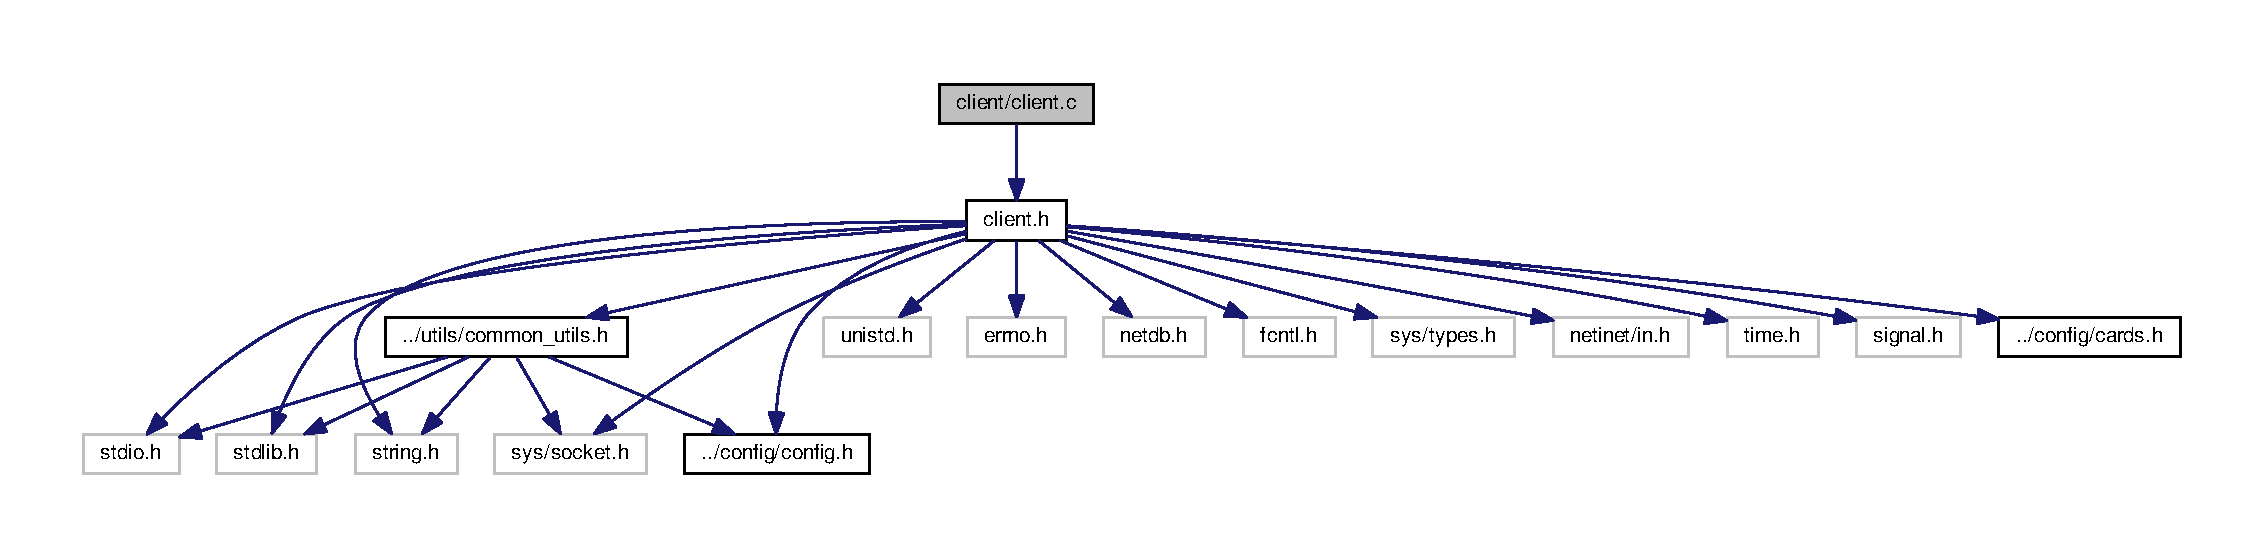
\includegraphics[width=350pt]{client_8c__incl}
\end{center}
\end{figure}
\subsection*{Functions}
\begin{DoxyCompactItemize}
\item 
void \hyperlink{client_8c_a4f63f6bd91eee4955bfb47c43c69580c}{disconnect} (\hyperlink{config_8h_a1062901a7428fdd9c7f180f5e01ea056}{bool} information)
\begin{DoxyCompactList}\small\item\em Fonction de déconnexion d\textquotesingle{}un client. \end{DoxyCompactList}\item 
void \hyperlink{client_8c_a1e135d989cd28349169939c6a73f2e87}{interrupt\+\_\+handler} (int signum)
\begin{DoxyCompactList}\small\item\em Fonction de déconnexion d\textquotesingle{}un client suita à un controle C. \end{DoxyCompactList}\item 
void \hyperlink{client_8c_a55a92a02360355337f5b149add054789}{refill} ()
\begin{DoxyCompactList}\small\item\em Fonction qui va remettre des cartes en jeu. \end{DoxyCompactList}\item 
void \hyperlink{client_8c_ae4e7472a72b57c06f73a935270a8a7b4}{clear\+\_\+cards} ()
\begin{DoxyCompactList}\small\item\em Fonction de nettoyage du buffer au niveau des cartes. \end{DoxyCompactList}\item 
void \hyperlink{client_8c_a58933b3f31fdb65d7b59f2075ac45564}{print\+\_\+cards} ()
\begin{DoxyCompactList}\small\item\em Fonction qui va afficher les cartes en jeu. \end{DoxyCompactList}\item 
int \hyperlink{client_8c_a7242a57cde933c761f8299e8decaf1de}{calculate\+\_\+score} ()
\begin{DoxyCompactList}\small\item\em Fonction qui va calculer le score. \end{DoxyCompactList}\item 
void \hyperlink{client_8c_ae27c64803e65cc4b90c30a03a213aa6b}{receive\+\_\+message} (int \hyperlink{client_8c_ae887b77f939a43b6387aa460f46836eb}{client\+\_\+socket}, char $\ast$$\ast$name)
\begin{DoxyCompactList}\small\item\em Fonction qui va envoyer ua client un message du serveur en fonction des configs données. \end{DoxyCompactList}\item 
void \hyperlink{client_8c_adc564b1835274102115eb7e5969dadc5}{create\+\_\+nickname} (char $\ast$name)
\begin{DoxyCompactList}\small\item\em Fonction qui va créer un pseudo à un joueur. \end{DoxyCompactList}\item 
void \hyperlink{client_8c_a32641083b53a88465743f059fa60c984}{connect\+To\+Server} (int $\ast$\hyperlink{client_8c_ae887b77f939a43b6387aa460f46836eb}{client\+\_\+socket}, char $\ast$server\+\_\+ip, struct hostent $\ast$host, struct sockaddr\+\_\+in $\ast$server\+\_\+address)
\begin{DoxyCompactList}\small\item\em Fonction qui va nous connecter à un serveur. \end{DoxyCompactList}\item 
\hyperlink{config_8h_a1062901a7428fdd9c7f180f5e01ea056}{bool} \hyperlink{client_8c_a7bf4695f7782c334645514191cf18750}{fdp\+\_\+is\+\_\+valid} (int fdp)
\item 
int \hyperlink{client_8c_a94769cbc8673a692eebd5ce12a9b6663}{rand\+\_\+range} (int upper\+\_\+limit)
\begin{DoxyCompactList}\small\item\em Fonction qui génère un nombre aléatoire dans le max de upperlimite. \end{DoxyCompactList}\item 
int \hyperlink{client_8c_a0ddf1224851353fc92bfbff6f499fa97}{main} (int argc, char $\ast$argv\mbox{[}$\,$\mbox{]})
\end{DoxyCompactItemize}
\subsection*{Variables}
\begin{DoxyCompactItemize}
\item 
int \hyperlink{client_8c_ae887b77f939a43b6387aa460f46836eb}{client\+\_\+socket}
\item 
int \hyperlink{client_8c_ac4a56f04e7cabfc5f4c467012f09d0f6}{hand} \mbox{[}\hyperlink{cards_8h_ab48a679225d82ec51e09e62d14313b34}{D\+E\+C\+K\+\_\+\+S\+I\+ZE}\mbox{]}
\item 
int \hyperlink{client_8c_a5f9a33eb1ad49eebc1c135f8e40762d0}{hand\+\_\+white} \mbox{[}\hyperlink{cards_8h_a308b28964d4d62d9376f756452df40fe}{D\+E\+C\+K\+\_\+\+S\+I\+Z\+E\+\_\+\+W\+H\+I\+TE}\mbox{]}
\item 
int \hyperlink{client_8c_af046b053e2ec02e26b5431c503a04793}{stash} \mbox{[}\hyperlink{cards_8h_ab48a679225d82ec51e09e62d14313b34}{D\+E\+C\+K\+\_\+\+S\+I\+ZE}\mbox{]}
\item 
int \hyperlink{client_8c_a741de07159ef83402d83a903405297d1}{cards\+\_\+in\+\_\+hand}
\item 
int \hyperlink{client_8c_a11bc9b70a69390634d42f6cb35569b4c}{cards\+\_\+in\+\_\+stash}
\end{DoxyCompactItemize}


\subsection{Detailed Description}
Projet de M\+C\+S3 2016 2017. 

\begin{DoxyAuthor}{Author}
B\+E\+N\+C\+H\+I\+HA -\/ S\+A\+L\+E\+N\+G\+RO -\/ L\+E\+F\+O\+RT 
\end{DoxyAuthor}
\begin{DoxyVersion}{Version}
1 
\end{DoxyVersion}
\begin{DoxyDate}{Date}
D\+E\+C\+E\+M\+B\+RE -\/ J\+A\+N\+V\+I\+ER
\end{DoxyDate}
Fichier gérant le client du projet 

\subsection{Function Documentation}
\index{client.\+c@{client.\+c}!calculate\+\_\+score@{calculate\+\_\+score}}
\index{calculate\+\_\+score@{calculate\+\_\+score}!client.\+c@{client.\+c}}
\subsubsection[{\texorpdfstring{calculate\+\_\+score()}{calculate_score()}}]{\setlength{\rightskip}{0pt plus 5cm}int calculate\+\_\+score (
\begin{DoxyParamCaption}
{}
\end{DoxyParamCaption}
)}\hypertarget{client_8c_a7242a57cde933c761f8299e8decaf1de}{}\label{client_8c_a7242a57cde933c761f8299e8decaf1de}


Fonction qui va calculer le score. 


\begin{DoxyParams}{Parameters}
{\em void} & \\
\hline
\end{DoxyParams}
\begin{DoxyReturn}{Returns}
score. 
\end{DoxyReturn}
\index{client.\+c@{client.\+c}!clear\+\_\+cards@{clear\+\_\+cards}}
\index{clear\+\_\+cards@{clear\+\_\+cards}!client.\+c@{client.\+c}}
\subsubsection[{\texorpdfstring{clear\+\_\+cards()}{clear_cards()}}]{\setlength{\rightskip}{0pt plus 5cm}void clear\+\_\+cards (
\begin{DoxyParamCaption}
{}
\end{DoxyParamCaption}
)}\hypertarget{client_8c_ae4e7472a72b57c06f73a935270a8a7b4}{}\label{client_8c_ae4e7472a72b57c06f73a935270a8a7b4}


Fonction de nettoyage du buffer au niveau des cartes. 


\begin{DoxyParams}{Parameters}
{\em void} & \\
\hline
\end{DoxyParams}
\begin{DoxyReturn}{Returns}
V\+O\+ID. 
\end{DoxyReturn}
\index{client.\+c@{client.\+c}!connect\+To\+Server@{connect\+To\+Server}}
\index{connect\+To\+Server@{connect\+To\+Server}!client.\+c@{client.\+c}}
\subsubsection[{\texorpdfstring{connect\+To\+Server(int $\ast$client\+\_\+socket, char $\ast$server\+\_\+ip, struct hostent $\ast$host, struct sockaddr\+\_\+in $\ast$server\+\_\+address)}{connectToServer(int *client_socket, char *server_ip, struct hostent *host, struct sockaddr_in *server_address)}}]{\setlength{\rightskip}{0pt plus 5cm}void connect\+To\+Server (
\begin{DoxyParamCaption}
\item[{int $\ast$}]{client\+\_\+socket, }
\item[{char $\ast$}]{server\+\_\+ip, }
\item[{struct hostent $\ast$}]{host, }
\item[{struct sockaddr\+\_\+in $\ast$}]{server\+\_\+address}
\end{DoxyParamCaption}
)}\hypertarget{client_8c_a32641083b53a88465743f059fa60c984}{}\label{client_8c_a32641083b53a88465743f059fa60c984}


Fonction qui va nous connecter à un serveur. 


\begin{DoxyParams}{Parameters}
{\em $\ast$client\+\_\+socket} & \\
\hline
{\em $\ast$server\+\_\+ip} & \\
\hline
{\em $\ast$host} & \\
\hline
{\em $\ast$server\+\_\+address} & \\
\hline
\end{DoxyParams}
\begin{DoxyReturn}{Returns}
V\+O\+ID. 
\end{DoxyReturn}
\index{client.\+c@{client.\+c}!create\+\_\+nickname@{create\+\_\+nickname}}
\index{create\+\_\+nickname@{create\+\_\+nickname}!client.\+c@{client.\+c}}
\subsubsection[{\texorpdfstring{create\+\_\+nickname(char $\ast$name)}{create_nickname(char *name)}}]{\setlength{\rightskip}{0pt plus 5cm}void create\+\_\+nickname (
\begin{DoxyParamCaption}
\item[{char $\ast$}]{name}
\end{DoxyParamCaption}
)}\hypertarget{client_8c_adc564b1835274102115eb7e5969dadc5}{}\label{client_8c_adc564b1835274102115eb7e5969dadc5}


Fonction qui va créer un pseudo à un joueur. 


\begin{DoxyParams}{Parameters}
{\em $\ast$name} & \\
\hline
\end{DoxyParams}
\begin{DoxyReturn}{Returns}
V\+O\+ID. 
\end{DoxyReturn}
\index{client.\+c@{client.\+c}!disconnect@{disconnect}}
\index{disconnect@{disconnect}!client.\+c@{client.\+c}}
\subsubsection[{\texorpdfstring{disconnect(bool information)}{disconnect(bool information)}}]{\setlength{\rightskip}{0pt plus 5cm}void disconnect (
\begin{DoxyParamCaption}
\item[{{\bf bool}}]{information}
\end{DoxyParamCaption}
)}\hypertarget{client_8c_a4f63f6bd91eee4955bfb47c43c69580c}{}\label{client_8c_a4f63f6bd91eee4955bfb47c43c69580c}


Fonction de déconnexion d\textquotesingle{}un client. 


\begin{DoxyParams}{Parameters}
{\em information} & boolean qui va vérifier si on s\textquotesingle{}est déconnecté ou pas. \\
\hline
\end{DoxyParams}
\begin{DoxyReturn}{Returns}
V\+O\+ID 
\end{DoxyReturn}
\index{client.\+c@{client.\+c}!fdp\+\_\+is\+\_\+valid@{fdp\+\_\+is\+\_\+valid}}
\index{fdp\+\_\+is\+\_\+valid@{fdp\+\_\+is\+\_\+valid}!client.\+c@{client.\+c}}
\subsubsection[{\texorpdfstring{fdp\+\_\+is\+\_\+valid(int fdp)}{fdp_is_valid(int fdp)}}]{\setlength{\rightskip}{0pt plus 5cm}{\bf bool} fdp\+\_\+is\+\_\+valid (
\begin{DoxyParamCaption}
\item[{int}]{fdp}
\end{DoxyParamCaption}
)}\hypertarget{client_8c_a7bf4695f7782c334645514191cf18750}{}\label{client_8c_a7bf4695f7782c334645514191cf18750}
\index{client.\+c@{client.\+c}!interrupt\+\_\+handler@{interrupt\+\_\+handler}}
\index{interrupt\+\_\+handler@{interrupt\+\_\+handler}!client.\+c@{client.\+c}}
\subsubsection[{\texorpdfstring{interrupt\+\_\+handler(int signum)}{interrupt_handler(int signum)}}]{\setlength{\rightskip}{0pt plus 5cm}void interrupt\+\_\+handler (
\begin{DoxyParamCaption}
\item[{int}]{signum}
\end{DoxyParamCaption}
)}\hypertarget{client_8c_a1e135d989cd28349169939c6a73f2e87}{}\label{client_8c_a1e135d989cd28349169939c6a73f2e87}


Fonction de déconnexion d\textquotesingle{}un client suita à un controle C. 

Fonction de signal d\textquotesingle{}interruption.


\begin{DoxyParams}{Parameters}
{\em signum} & signal vérifiant le controle C \\
\hline
\end{DoxyParams}
\begin{DoxyReturn}{Returns}
V\+O\+ID.
\end{DoxyReturn}

\begin{DoxyParams}{Parameters}
{\em signum} & \\
\hline
\end{DoxyParams}
\begin{DoxyReturn}{Returns}
V\+O\+ID 
\end{DoxyReturn}
\index{client.\+c@{client.\+c}!main@{main}}
\index{main@{main}!client.\+c@{client.\+c}}
\subsubsection[{\texorpdfstring{main(int argc, char $\ast$argv[])}{main(int argc, char *argv[])}}]{\setlength{\rightskip}{0pt plus 5cm}int main (
\begin{DoxyParamCaption}
\item[{int}]{argc, }
\item[{char $\ast$}]{argv\mbox{[}$\,$\mbox{]}}
\end{DoxyParamCaption}
)}\hypertarget{client_8c_a0ddf1224851353fc92bfbff6f499fa97}{}\label{client_8c_a0ddf1224851353fc92bfbff6f499fa97}
\index{client.\+c@{client.\+c}!print\+\_\+cards@{print\+\_\+cards}}
\index{print\+\_\+cards@{print\+\_\+cards}!client.\+c@{client.\+c}}
\subsubsection[{\texorpdfstring{print\+\_\+cards()}{print_cards()}}]{\setlength{\rightskip}{0pt plus 5cm}void print\+\_\+cards (
\begin{DoxyParamCaption}
{}
\end{DoxyParamCaption}
)}\hypertarget{client_8c_a58933b3f31fdb65d7b59f2075ac45564}{}\label{client_8c_a58933b3f31fdb65d7b59f2075ac45564}


Fonction qui va afficher les cartes en jeu. 


\begin{DoxyParams}{Parameters}
{\em void} & \\
\hline
\end{DoxyParams}
\begin{DoxyReturn}{Returns}
V\+O\+ID. 
\end{DoxyReturn}
\index{client.\+c@{client.\+c}!rand\+\_\+range@{rand\+\_\+range}}
\index{rand\+\_\+range@{rand\+\_\+range}!client.\+c@{client.\+c}}
\subsubsection[{\texorpdfstring{rand\+\_\+range(int upper\+\_\+limit)}{rand_range(int upper_limit)}}]{\setlength{\rightskip}{0pt plus 5cm}rand\+\_\+range (
\begin{DoxyParamCaption}
\item[{int}]{upper\+\_\+limit}
\end{DoxyParamCaption}
)}\hypertarget{client_8c_a94769cbc8673a692eebd5ce12a9b6663}{}\label{client_8c_a94769cbc8673a692eebd5ce12a9b6663}


Fonction qui génère un nombre aléatoire dans le max de upperlimite. 

Fonction qui vérifie si une carte est présente dans le tableau.


\begin{DoxyParams}{Parameters}
{\em upper\+\_\+limit} & \\
\hline
\end{DoxyParams}
\begin{DoxyReturn}{Returns}
int
\end{DoxyReturn}

\begin{DoxyParams}{Parameters}
{\em $\ast$haystack} & \\
\hline
{\em needle} & \\
\hline
{\em length} & \\
\hline
\end{DoxyParams}
\begin{DoxyReturn}{Returns}
bool 
\end{DoxyReturn}
\index{client.\+c@{client.\+c}!receive\+\_\+message@{receive\+\_\+message}}
\index{receive\+\_\+message@{receive\+\_\+message}!client.\+c@{client.\+c}}
\subsubsection[{\texorpdfstring{receive\+\_\+message(int client\+\_\+socket, char $\ast$$\ast$name)}{receive_message(int client_socket, char **name)}}]{\setlength{\rightskip}{0pt plus 5cm}void receive\+\_\+message (
\begin{DoxyParamCaption}
\item[{int}]{client\+\_\+socket, }
\item[{char $\ast$$\ast$}]{name}
\end{DoxyParamCaption}
)}\hypertarget{client_8c_ae27c64803e65cc4b90c30a03a213aa6b}{}\label{client_8c_ae27c64803e65cc4b90c30a03a213aa6b}


Fonction qui va envoyer ua client un message du serveur en fonction des configs données. 


\begin{DoxyParams}{Parameters}
{\em client\+\_\+socket} & \\
\hline
{\em $\ast$$\ast$name} & \\
\hline
\end{DoxyParams}
\begin{DoxyReturn}{Returns}
V\+O\+ID. 
\end{DoxyReturn}
\index{client.\+c@{client.\+c}!refill@{refill}}
\index{refill@{refill}!client.\+c@{client.\+c}}
\subsubsection[{\texorpdfstring{refill()}{refill()}}]{\setlength{\rightskip}{0pt plus 5cm}void refill (
\begin{DoxyParamCaption}
{}
\end{DoxyParamCaption}
)}\hypertarget{client_8c_a55a92a02360355337f5b149add054789}{}\label{client_8c_a55a92a02360355337f5b149add054789}


Fonction qui va remettre des cartes en jeu. 


\begin{DoxyParams}{Parameters}
{\em void} & \\
\hline
\end{DoxyParams}
\begin{DoxyReturn}{Returns}
V\+O\+ID. 
\end{DoxyReturn}


\subsection{Variable Documentation}
\index{client.\+c@{client.\+c}!cards\+\_\+in\+\_\+hand@{cards\+\_\+in\+\_\+hand}}
\index{cards\+\_\+in\+\_\+hand@{cards\+\_\+in\+\_\+hand}!client.\+c@{client.\+c}}
\subsubsection[{\texorpdfstring{cards\+\_\+in\+\_\+hand}{cards_in_hand}}]{\setlength{\rightskip}{0pt plus 5cm}int cards\+\_\+in\+\_\+hand}\hypertarget{client_8c_a741de07159ef83402d83a903405297d1}{}\label{client_8c_a741de07159ef83402d83a903405297d1}
\index{client.\+c@{client.\+c}!cards\+\_\+in\+\_\+stash@{cards\+\_\+in\+\_\+stash}}
\index{cards\+\_\+in\+\_\+stash@{cards\+\_\+in\+\_\+stash}!client.\+c@{client.\+c}}
\subsubsection[{\texorpdfstring{cards\+\_\+in\+\_\+stash}{cards_in_stash}}]{\setlength{\rightskip}{0pt plus 5cm}int cards\+\_\+in\+\_\+stash}\hypertarget{client_8c_a11bc9b70a69390634d42f6cb35569b4c}{}\label{client_8c_a11bc9b70a69390634d42f6cb35569b4c}
\index{client.\+c@{client.\+c}!client\+\_\+socket@{client\+\_\+socket}}
\index{client\+\_\+socket@{client\+\_\+socket}!client.\+c@{client.\+c}}
\subsubsection[{\texorpdfstring{client\+\_\+socket}{client_socket}}]{\setlength{\rightskip}{0pt plus 5cm}int client\+\_\+socket}\hypertarget{client_8c_ae887b77f939a43b6387aa460f46836eb}{}\label{client_8c_ae887b77f939a43b6387aa460f46836eb}
\index{client.\+c@{client.\+c}!hand@{hand}}
\index{hand@{hand}!client.\+c@{client.\+c}}
\subsubsection[{\texorpdfstring{hand}{hand}}]{\setlength{\rightskip}{0pt plus 5cm}int hand\mbox{[}{\bf D\+E\+C\+K\+\_\+\+S\+I\+ZE}\mbox{]}}\hypertarget{client_8c_ac4a56f04e7cabfc5f4c467012f09d0f6}{}\label{client_8c_ac4a56f04e7cabfc5f4c467012f09d0f6}
\index{client.\+c@{client.\+c}!hand\+\_\+white@{hand\+\_\+white}}
\index{hand\+\_\+white@{hand\+\_\+white}!client.\+c@{client.\+c}}
\subsubsection[{\texorpdfstring{hand\+\_\+white}{hand_white}}]{\setlength{\rightskip}{0pt plus 5cm}int hand\+\_\+white\mbox{[}{\bf D\+E\+C\+K\+\_\+\+S\+I\+Z\+E\+\_\+\+W\+H\+I\+TE}\mbox{]}}\hypertarget{client_8c_a5f9a33eb1ad49eebc1c135f8e40762d0}{}\label{client_8c_a5f9a33eb1ad49eebc1c135f8e40762d0}
\index{client.\+c@{client.\+c}!stash@{stash}}
\index{stash@{stash}!client.\+c@{client.\+c}}
\subsubsection[{\texorpdfstring{stash}{stash}}]{\setlength{\rightskip}{0pt plus 5cm}int stash\mbox{[}{\bf D\+E\+C\+K\+\_\+\+S\+I\+ZE}\mbox{]}}\hypertarget{client_8c_af046b053e2ec02e26b5431c503a04793}{}\label{client_8c_af046b053e2ec02e26b5431c503a04793}

\hypertarget{client_8h}{}\section{client/client.h File Reference}
\label{client_8h}\index{client/client.\+h@{client/client.\+h}}
{\ttfamily \#include $<$stdio.\+h$>$}\\*
{\ttfamily \#include $<$stdlib.\+h$>$}\\*
{\ttfamily \#include $<$unistd.\+h$>$}\\*
{\ttfamily \#include $<$errno.\+h$>$}\\*
{\ttfamily \#include $<$string.\+h$>$}\\*
{\ttfamily \#include $<$netdb.\+h$>$}\\*
{\ttfamily \#include $<$fcntl.\+h$>$}\\*
{\ttfamily \#include $<$sys/types.\+h$>$}\\*
{\ttfamily \#include $<$netinet/in.\+h$>$}\\*
{\ttfamily \#include $<$sys/socket.\+h$>$}\\*
{\ttfamily \#include $<$time.\+h$>$}\\*
{\ttfamily \#include $<$signal.\+h$>$}\\*
{\ttfamily \#include \char`\"{}../config/config.\+h\char`\"{}}\\*
{\ttfamily \#include \char`\"{}../utils/common\+\_\+utils.\+h\char`\"{}}\\*
{\ttfamily \#include \char`\"{}../config/cards.\+h\char`\"{}}\\*
Include dependency graph for client.\+h\+:
\nopagebreak
\begin{figure}[H]
\begin{center}
\leavevmode
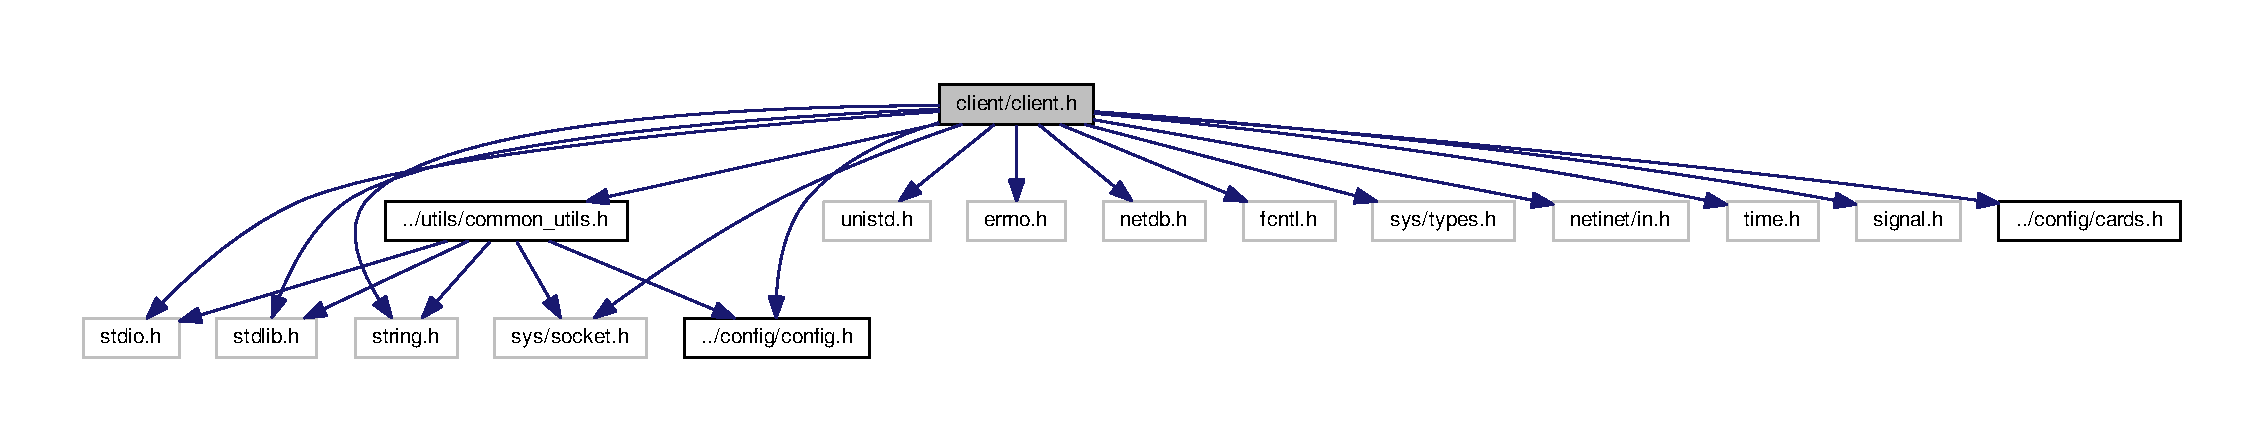
\includegraphics[width=350pt]{client_8h__incl}
\end{center}
\end{figure}
This graph shows which files directly or indirectly include this file\+:
\nopagebreak
\begin{figure}[H]
\begin{center}
\leavevmode
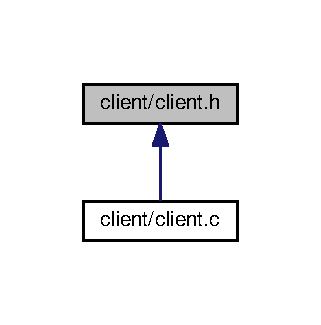
\includegraphics[width=154pt]{client_8h__dep__incl}
\end{center}
\end{figure}
\subsection*{Macros}
\begin{DoxyCompactItemize}
\item 
\#define \hyperlink{client_8h_a614217d263be1fb1a5f76e2ff7be19a2}{P\+O\+RT}~\hyperlink{ports_8h_a1725876d3b41d0601d59768e442b7907}{P\+O\+R\+T\+\_\+\+D\+I\+M\+OV}
\end{DoxyCompactItemize}
\subsection*{Functions}
\begin{DoxyCompactItemize}
\item 
void \hyperlink{client_8h_abcbf6c09394bb6a1db56ecf5c888fb87}{interrupt\+\_\+handler} (int)
\begin{DoxyCompactList}\small\item\em Fonction de déconnexion d\textquotesingle{}un client suita à un controle C. \end{DoxyCompactList}\item 
void \hyperlink{client_8h_a4f63f6bd91eee4955bfb47c43c69580c}{disconnect} (\hyperlink{config_8h_a1062901a7428fdd9c7f180f5e01ea056}{bool} information)
\begin{DoxyCompactList}\small\item\em Fonction de déconnexion d\textquotesingle{}un client. \end{DoxyCompactList}\item 
void \hyperlink{client_8h_a55a92a02360355337f5b149add054789}{refill} ()
\begin{DoxyCompactList}\small\item\em Fonction qui va remettre des cartes en jeu. \end{DoxyCompactList}\item 
void \hyperlink{client_8h_ae4e7472a72b57c06f73a935270a8a7b4}{clear\+\_\+cards} ()
\begin{DoxyCompactList}\small\item\em Fonction de nettoyage du buffer au niveau des cartes. \end{DoxyCompactList}\item 
void \hyperlink{client_8h_a58933b3f31fdb65d7b59f2075ac45564}{print\+\_\+cards} ()
\begin{DoxyCompactList}\small\item\em Fonction qui va afficher les cartes en jeu. \end{DoxyCompactList}\item 
int \hyperlink{client_8h_a7242a57cde933c761f8299e8decaf1de}{calculate\+\_\+score} ()
\begin{DoxyCompactList}\small\item\em Fonction qui va calculer le score. \end{DoxyCompactList}\item 
void \hyperlink{client_8h_a1f3011f48a3802fe92ca6576022f023a}{receive\+\_\+message} (int client\+Socket, char $\ast$$\ast$name)
\begin{DoxyCompactList}\small\item\em Fonction qui va envoyer ua client un message du serveur en fonction des configs données. \end{DoxyCompactList}\item 
void \hyperlink{client_8h_a13d44c296ab00e94f7210c883b12c83d}{create\+Nickname} (char $\ast$name)
\item 
void \hyperlink{client_8h_a678b30449c0a2fde55ebf0dc66552c4c}{connect\+To\+Server} (int $\ast$client\+Socket, char $\ast$server\+IP, struct hostent $\ast$he, struct sockaddr\+\_\+in $\ast$server\+Address)
\begin{DoxyCompactList}\small\item\em Fonction qui va nous connecter à un serveur. \end{DoxyCompactList}\item 
\hyperlink{config_8h_a1062901a7428fdd9c7f180f5e01ea056}{bool} \hyperlink{client_8h_a7bf4695f7782c334645514191cf18750}{fdp\+\_\+is\+\_\+valid} (int fdp)
\end{DoxyCompactItemize}


\subsection{Macro Definition Documentation}
\index{client.\+h@{client.\+h}!P\+O\+RT@{P\+O\+RT}}
\index{P\+O\+RT@{P\+O\+RT}!client.\+h@{client.\+h}}
\subsubsection[{\texorpdfstring{P\+O\+RT}{PORT}}]{\setlength{\rightskip}{0pt plus 5cm}\#define P\+O\+RT~{\bf P\+O\+R\+T\+\_\+\+D\+I\+M\+OV}}\hypertarget{client_8h_a614217d263be1fb1a5f76e2ff7be19a2}{}\label{client_8h_a614217d263be1fb1a5f76e2ff7be19a2}


\subsection{Function Documentation}
\index{client.\+h@{client.\+h}!calculate\+\_\+score@{calculate\+\_\+score}}
\index{calculate\+\_\+score@{calculate\+\_\+score}!client.\+h@{client.\+h}}
\subsubsection[{\texorpdfstring{calculate\+\_\+score()}{calculate_score()}}]{\setlength{\rightskip}{0pt plus 5cm}int calculate\+\_\+score (
\begin{DoxyParamCaption}
{}
\end{DoxyParamCaption}
)}\hypertarget{client_8h_a7242a57cde933c761f8299e8decaf1de}{}\label{client_8h_a7242a57cde933c761f8299e8decaf1de}


Fonction qui va calculer le score. 


\begin{DoxyParams}{Parameters}
{\em void} & \\
\hline
\end{DoxyParams}
\begin{DoxyReturn}{Returns}
score. 
\end{DoxyReturn}
\index{client.\+h@{client.\+h}!clear\+\_\+cards@{clear\+\_\+cards}}
\index{clear\+\_\+cards@{clear\+\_\+cards}!client.\+h@{client.\+h}}
\subsubsection[{\texorpdfstring{clear\+\_\+cards()}{clear_cards()}}]{\setlength{\rightskip}{0pt plus 5cm}void clear\+\_\+cards (
\begin{DoxyParamCaption}
{}
\end{DoxyParamCaption}
)}\hypertarget{client_8h_ae4e7472a72b57c06f73a935270a8a7b4}{}\label{client_8h_ae4e7472a72b57c06f73a935270a8a7b4}


Fonction de nettoyage du buffer au niveau des cartes. 


\begin{DoxyParams}{Parameters}
{\em void} & \\
\hline
\end{DoxyParams}
\begin{DoxyReturn}{Returns}
V\+O\+ID. 
\end{DoxyReturn}
\index{client.\+h@{client.\+h}!connect\+To\+Server@{connect\+To\+Server}}
\index{connect\+To\+Server@{connect\+To\+Server}!client.\+h@{client.\+h}}
\subsubsection[{\texorpdfstring{connect\+To\+Server(int $\ast$client\+Socket, char $\ast$server\+I\+P, struct hostent $\ast$he, struct sockaddr\+\_\+in $\ast$server\+Address)}{connectToServer(int *clientSocket, char *serverIP, struct hostent *he, struct sockaddr_in *serverAddress)}}]{\setlength{\rightskip}{0pt plus 5cm}void connect\+To\+Server (
\begin{DoxyParamCaption}
\item[{int $\ast$}]{client\+\_\+socket, }
\item[{char $\ast$}]{server\+\_\+ip, }
\item[{struct hostent $\ast$}]{host, }
\item[{struct sockaddr\+\_\+in $\ast$}]{server\+\_\+address}
\end{DoxyParamCaption}
)}\hypertarget{client_8h_a678b30449c0a2fde55ebf0dc66552c4c}{}\label{client_8h_a678b30449c0a2fde55ebf0dc66552c4c}


Fonction qui va nous connecter à un serveur. 


\begin{DoxyParams}{Parameters}
{\em $\ast$client\+\_\+socket} & \\
\hline
{\em $\ast$server\+\_\+ip} & \\
\hline
{\em $\ast$host} & \\
\hline
{\em $\ast$server\+\_\+address} & \\
\hline
\end{DoxyParams}
\begin{DoxyReturn}{Returns}
V\+O\+ID. 
\end{DoxyReturn}
\index{client.\+h@{client.\+h}!create\+Nickname@{create\+Nickname}}
\index{create\+Nickname@{create\+Nickname}!client.\+h@{client.\+h}}
\subsubsection[{\texorpdfstring{create\+Nickname(char $\ast$name)}{createNickname(char *name)}}]{\setlength{\rightskip}{0pt plus 5cm}void create\+Nickname (
\begin{DoxyParamCaption}
\item[{char $\ast$}]{name}
\end{DoxyParamCaption}
)}\hypertarget{client_8h_a13d44c296ab00e94f7210c883b12c83d}{}\label{client_8h_a13d44c296ab00e94f7210c883b12c83d}
\index{client.\+h@{client.\+h}!disconnect@{disconnect}}
\index{disconnect@{disconnect}!client.\+h@{client.\+h}}
\subsubsection[{\texorpdfstring{disconnect(bool information)}{disconnect(bool information)}}]{\setlength{\rightskip}{0pt plus 5cm}void disconnect (
\begin{DoxyParamCaption}
\item[{{\bf bool}}]{information}
\end{DoxyParamCaption}
)}\hypertarget{client_8h_a4f63f6bd91eee4955bfb47c43c69580c}{}\label{client_8h_a4f63f6bd91eee4955bfb47c43c69580c}


Fonction de déconnexion d\textquotesingle{}un client. 


\begin{DoxyParams}{Parameters}
{\em information} & boolean qui va vérifier si on s\textquotesingle{}est déconnecté ou pas. \\
\hline
\end{DoxyParams}
\begin{DoxyReturn}{Returns}
V\+O\+ID 
\end{DoxyReturn}
\index{client.\+h@{client.\+h}!fdp\+\_\+is\+\_\+valid@{fdp\+\_\+is\+\_\+valid}}
\index{fdp\+\_\+is\+\_\+valid@{fdp\+\_\+is\+\_\+valid}!client.\+h@{client.\+h}}
\subsubsection[{\texorpdfstring{fdp\+\_\+is\+\_\+valid(int fdp)}{fdp_is_valid(int fdp)}}]{\setlength{\rightskip}{0pt plus 5cm}{\bf bool} fdp\+\_\+is\+\_\+valid (
\begin{DoxyParamCaption}
\item[{int}]{fdp}
\end{DoxyParamCaption}
)}\hypertarget{client_8h_a7bf4695f7782c334645514191cf18750}{}\label{client_8h_a7bf4695f7782c334645514191cf18750}
\index{client.\+h@{client.\+h}!interrupt\+\_\+handler@{interrupt\+\_\+handler}}
\index{interrupt\+\_\+handler@{interrupt\+\_\+handler}!client.\+h@{client.\+h}}
\subsubsection[{\texorpdfstring{interrupt\+\_\+handler(int)}{interrupt_handler(int)}}]{\setlength{\rightskip}{0pt plus 5cm}void interrupt\+\_\+handler (
\begin{DoxyParamCaption}
\item[{int}]{signum}
\end{DoxyParamCaption}
)}\hypertarget{client_8h_abcbf6c09394bb6a1db56ecf5c888fb87}{}\label{client_8h_abcbf6c09394bb6a1db56ecf5c888fb87}


Fonction de déconnexion d\textquotesingle{}un client suita à un controle C. 

Fonction de signal d\textquotesingle{}interruption.


\begin{DoxyParams}{Parameters}
{\em signum} & signal vérifiant le controle C \\
\hline
\end{DoxyParams}
\begin{DoxyReturn}{Returns}
V\+O\+ID.
\end{DoxyReturn}

\begin{DoxyParams}{Parameters}
{\em signum} & \\
\hline
\end{DoxyParams}
\begin{DoxyReturn}{Returns}
V\+O\+ID 
\end{DoxyReturn}
\index{client.\+h@{client.\+h}!print\+\_\+cards@{print\+\_\+cards}}
\index{print\+\_\+cards@{print\+\_\+cards}!client.\+h@{client.\+h}}
\subsubsection[{\texorpdfstring{print\+\_\+cards()}{print_cards()}}]{\setlength{\rightskip}{0pt plus 5cm}void print\+\_\+cards (
\begin{DoxyParamCaption}
{}
\end{DoxyParamCaption}
)}\hypertarget{client_8h_a58933b3f31fdb65d7b59f2075ac45564}{}\label{client_8h_a58933b3f31fdb65d7b59f2075ac45564}


Fonction qui va afficher les cartes en jeu. 


\begin{DoxyParams}{Parameters}
{\em void} & \\
\hline
\end{DoxyParams}
\begin{DoxyReturn}{Returns}
V\+O\+ID. 
\end{DoxyReturn}
\index{client.\+h@{client.\+h}!receive\+\_\+message@{receive\+\_\+message}}
\index{receive\+\_\+message@{receive\+\_\+message}!client.\+h@{client.\+h}}
\subsubsection[{\texorpdfstring{receive\+\_\+message(int client\+Socket, char $\ast$$\ast$name)}{receive_message(int clientSocket, char **name)}}]{\setlength{\rightskip}{0pt plus 5cm}void receive\+\_\+message (
\begin{DoxyParamCaption}
\item[{int}]{client\+\_\+socket, }
\item[{char $\ast$$\ast$}]{name}
\end{DoxyParamCaption}
)}\hypertarget{client_8h_a1f3011f48a3802fe92ca6576022f023a}{}\label{client_8h_a1f3011f48a3802fe92ca6576022f023a}


Fonction qui va envoyer ua client un message du serveur en fonction des configs données. 


\begin{DoxyParams}{Parameters}
{\em client\+\_\+socket} & \\
\hline
{\em $\ast$$\ast$name} & \\
\hline
\end{DoxyParams}
\begin{DoxyReturn}{Returns}
V\+O\+ID. 
\end{DoxyReturn}
\index{client.\+h@{client.\+h}!refill@{refill}}
\index{refill@{refill}!client.\+h@{client.\+h}}
\subsubsection[{\texorpdfstring{refill()}{refill()}}]{\setlength{\rightskip}{0pt plus 5cm}void refill (
\begin{DoxyParamCaption}
{}
\end{DoxyParamCaption}
)}\hypertarget{client_8h_a55a92a02360355337f5b149add054789}{}\label{client_8h_a55a92a02360355337f5b149add054789}


Fonction qui va remettre des cartes en jeu. 


\begin{DoxyParams}{Parameters}
{\em void} & \\
\hline
\end{DoxyParams}
\begin{DoxyReturn}{Returns}
V\+O\+ID. 
\end{DoxyReturn}

\hypertarget{cards_8c}{}\section{config/cards.c File Reference}
\label{cards_8c}\index{config/cards.\+c@{config/cards.\+c}}


Projet de M\+C\+S3 2016 2017.  


{\ttfamily \#include \char`\"{}cards.\+h\char`\"{}}\\*
Include dependency graph for cards.\+c\+:
\nopagebreak
\begin{figure}[H]
\begin{center}
\leavevmode
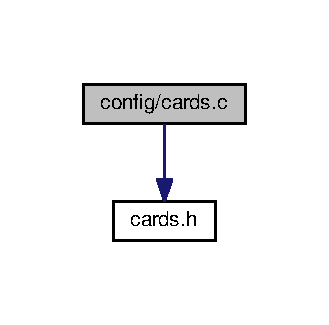
\includegraphics[width=158pt]{cards_8c__incl}
\end{center}
\end{figure}
\subsection*{Functions}
\begin{DoxyCompactItemize}
\item 
char $\ast$ \hyperlink{cards_8c_ab96f593fdc3e836e13c9bb86033d344b}{get\+\_\+card\+\_\+name} (int card)
\begin{DoxyCompactList}\small\item\em Fonction donnant le nom de la carte noire. \end{DoxyCompactList}\item 
char $\ast$ \hyperlink{cards_8c_a643c320012cc73bc25f416e523ce0b57}{get\+\_\+card\+\_\+white\+\_\+name} (int card)
\begin{DoxyCompactList}\small\item\em Fonction donnant le nom de la carte blanche. \end{DoxyCompactList}\item 
int \hyperlink{cards_8c_a03ca4a0d6d7efe075a2fc7cf069a6ce9}{get\+\_\+card\+\_\+points} (int card)
\end{DoxyCompactItemize}
\subsection*{Variables}
\begin{DoxyCompactItemize}
\item 
char $\ast$ \hyperlink{cards_8c_a509e584a2babf2e60eb4851ac6192c15}{card\+\_\+black\+\_\+names} \mbox{[}$\,$\mbox{]}
\item 
char $\ast$ \hyperlink{cards_8c_a4c59b4d7538c8888ac236a755adcd6a7}{card\+\_\+white\+\_\+names} \mbox{[}$\,$\mbox{]}
\end{DoxyCompactItemize}


\subsection{Detailed Description}
Projet de M\+C\+S3 2016 2017. 

\begin{DoxyAuthor}{Author}
B\+E\+N\+C\+H\+I\+HA -\/ S\+A\+L\+E\+N\+G\+RO -\/ L\+E\+F\+O\+RT 
\end{DoxyAuthor}
\begin{DoxyVersion}{Version}
1 
\end{DoxyVersion}
\begin{DoxyDate}{Date}
D\+E\+C\+E\+M\+B\+RE -\/ J\+A\+N\+V\+I\+ER
\end{DoxyDate}
Fichier gérant les cartes du jeu 

\subsection{Function Documentation}
\index{cards.\+c@{cards.\+c}!get\+\_\+card\+\_\+name@{get\+\_\+card\+\_\+name}}
\index{get\+\_\+card\+\_\+name@{get\+\_\+card\+\_\+name}!cards.\+c@{cards.\+c}}
\subsubsection[{\texorpdfstring{get\+\_\+card\+\_\+name(int card)}{get_card_name(int card)}}]{\setlength{\rightskip}{0pt plus 5cm}char $\ast$ get\+\_\+card\+\_\+name (
\begin{DoxyParamCaption}
\item[{int}]{card}
\end{DoxyParamCaption}
)}\hypertarget{cards_8c_ab96f593fdc3e836e13c9bb86033d344b}{}\label{cards_8c_ab96f593fdc3e836e13c9bb86033d344b}


Fonction donnant le nom de la carte noire. 

Fonction donnant les points d\textquotesingle{}une cartes.


\begin{DoxyParams}{Parameters}
{\em card} & \\
\hline
\end{DoxyParams}
\begin{DoxyReturn}{Returns}
char$\ast$
\end{DoxyReturn}

\begin{DoxyParams}{Parameters}
{\em card} & \\
\hline
\end{DoxyParams}
\begin{DoxyReturn}{Returns}
int 
\end{DoxyReturn}
\index{cards.\+c@{cards.\+c}!get\+\_\+card\+\_\+points@{get\+\_\+card\+\_\+points}}
\index{get\+\_\+card\+\_\+points@{get\+\_\+card\+\_\+points}!cards.\+c@{cards.\+c}}
\subsubsection[{\texorpdfstring{get\+\_\+card\+\_\+points(int card)}{get_card_points(int card)}}]{\setlength{\rightskip}{0pt plus 5cm}int get\+\_\+card\+\_\+points (
\begin{DoxyParamCaption}
\item[{int}]{card}
\end{DoxyParamCaption}
)}\hypertarget{cards_8c_a03ca4a0d6d7efe075a2fc7cf069a6ce9}{}\label{cards_8c_a03ca4a0d6d7efe075a2fc7cf069a6ce9}
Chaque carte à des points \index{cards.\+c@{cards.\+c}!get\+\_\+card\+\_\+white\+\_\+name@{get\+\_\+card\+\_\+white\+\_\+name}}
\index{get\+\_\+card\+\_\+white\+\_\+name@{get\+\_\+card\+\_\+white\+\_\+name}!cards.\+c@{cards.\+c}}
\subsubsection[{\texorpdfstring{get\+\_\+card\+\_\+white\+\_\+name(int card)}{get_card_white_name(int card)}}]{\setlength{\rightskip}{0pt plus 5cm}char $\ast$ get\+\_\+card\+\_\+white\+\_\+name (
\begin{DoxyParamCaption}
\item[{int}]{card}
\end{DoxyParamCaption}
)}\hypertarget{cards_8c_a643c320012cc73bc25f416e523ce0b57}{}\label{cards_8c_a643c320012cc73bc25f416e523ce0b57}


Fonction donnant le nom de la carte blanche. 


\begin{DoxyParams}{Parameters}
{\em card} & \\
\hline
\end{DoxyParams}
\begin{DoxyReturn}{Returns}
char$\ast$ 
\end{DoxyReturn}


\subsection{Variable Documentation}
\index{cards.\+c@{cards.\+c}!card\+\_\+black\+\_\+names@{card\+\_\+black\+\_\+names}}
\index{card\+\_\+black\+\_\+names@{card\+\_\+black\+\_\+names}!cards.\+c@{cards.\+c}}
\subsubsection[{\texorpdfstring{card\+\_\+black\+\_\+names}{card_black_names}}]{\setlength{\rightskip}{0pt plus 5cm}char$\ast$ card\+\_\+black\+\_\+names\mbox{[}$\,$\mbox{]}}\hypertarget{cards_8c_a509e584a2babf2e60eb4851ac6192c15}{}\label{cards_8c_a509e584a2babf2e60eb4851ac6192c15}
\index{cards.\+c@{cards.\+c}!card\+\_\+white\+\_\+names@{card\+\_\+white\+\_\+names}}
\index{card\+\_\+white\+\_\+names@{card\+\_\+white\+\_\+names}!cards.\+c@{cards.\+c}}
\subsubsection[{\texorpdfstring{card\+\_\+white\+\_\+names}{card_white_names}}]{\setlength{\rightskip}{0pt plus 5cm}char$\ast$ card\+\_\+white\+\_\+names\mbox{[}$\,$\mbox{]}}\hypertarget{cards_8c_a4c59b4d7538c8888ac236a755adcd6a7}{}\label{cards_8c_a4c59b4d7538c8888ac236a755adcd6a7}

\hypertarget{cards_8h}{}\section{config/cards.h File Reference}
\label{cards_8h}\index{config/cards.\+h@{config/cards.\+h}}


Projet de M\+C\+S3 2016 2017.  


This graph shows which files directly or indirectly include this file\+:
\nopagebreak
\begin{figure}[H]
\begin{center}
\leavevmode
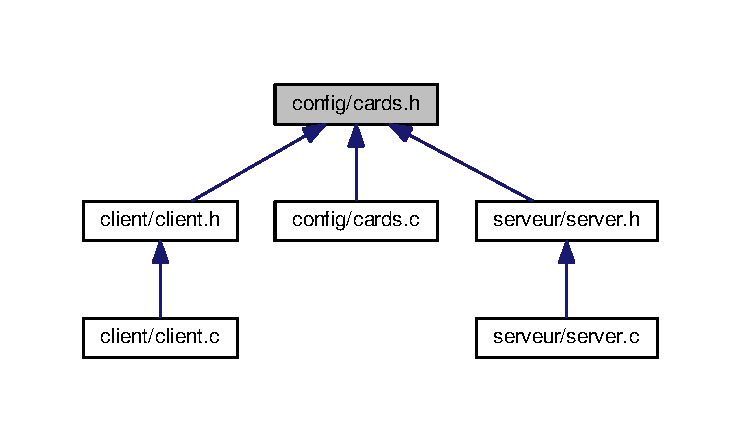
\includegraphics[width=350pt]{cards_8h__dep__incl}
\end{center}
\end{figure}
\subsection*{Macros}
\begin{DoxyCompactItemize}
\item 
\#define \hyperlink{cards_8h_ab48a679225d82ec51e09e62d14313b34}{D\+E\+C\+K\+\_\+\+S\+I\+ZE}~52
\item 
\#define \hyperlink{cards_8h_a308b28964d4d62d9376f756452df40fe}{D\+E\+C\+K\+\_\+\+S\+I\+Z\+E\+\_\+\+W\+H\+I\+TE}~52
\end{DoxyCompactItemize}
\subsection*{Functions}
\begin{DoxyCompactItemize}
\item 
char $\ast$ \hyperlink{cards_8h_a4a532cc5bc7bf712be21cc08f987242e}{get\+\_\+card\+\_\+name} (int card)
\begin{DoxyCompactList}\small\item\em Fonction donnant le nom de la carte noire. \end{DoxyCompactList}\item 
char $\ast$ \hyperlink{cards_8h_a5dec021eb3cd40a95ba812b1c0533d56}{get\+\_\+card\+\_\+white\+\_\+name} (int card)
\begin{DoxyCompactList}\small\item\em Fonction donnant le nom de la carte blanche. \end{DoxyCompactList}\item 
int \hyperlink{cards_8h_a03ca4a0d6d7efe075a2fc7cf069a6ce9}{get\+\_\+card\+\_\+points} (int card)
\end{DoxyCompactItemize}


\subsection{Detailed Description}
Projet de M\+C\+S3 2016 2017. 

\begin{DoxyAuthor}{Author}
B\+E\+N\+C\+H\+I\+HA -\/ S\+A\+L\+E\+N\+G\+RO -\/ L\+E\+F\+O\+RT 
\end{DoxyAuthor}
\begin{DoxyVersion}{Version}
1 
\end{DoxyVersion}
\begin{DoxyDate}{Date}
D\+E\+C\+E\+M\+B\+RE -\/ J\+A\+N\+V\+I\+ER
\end{DoxyDate}
Fichier gérant les cartes du jeu 

\subsection{Macro Definition Documentation}
\index{cards.\+h@{cards.\+h}!D\+E\+C\+K\+\_\+\+S\+I\+ZE@{D\+E\+C\+K\+\_\+\+S\+I\+ZE}}
\index{D\+E\+C\+K\+\_\+\+S\+I\+ZE@{D\+E\+C\+K\+\_\+\+S\+I\+ZE}!cards.\+h@{cards.\+h}}
\subsubsection[{\texorpdfstring{D\+E\+C\+K\+\_\+\+S\+I\+ZE}{DECK_SIZE}}]{\setlength{\rightskip}{0pt plus 5cm}\#define D\+E\+C\+K\+\_\+\+S\+I\+ZE~52}\hypertarget{cards_8h_ab48a679225d82ec51e09e62d14313b34}{}\label{cards_8h_ab48a679225d82ec51e09e62d14313b34}
\index{cards.\+h@{cards.\+h}!D\+E\+C\+K\+\_\+\+S\+I\+Z\+E\+\_\+\+W\+H\+I\+TE@{D\+E\+C\+K\+\_\+\+S\+I\+Z\+E\+\_\+\+W\+H\+I\+TE}}
\index{D\+E\+C\+K\+\_\+\+S\+I\+Z\+E\+\_\+\+W\+H\+I\+TE@{D\+E\+C\+K\+\_\+\+S\+I\+Z\+E\+\_\+\+W\+H\+I\+TE}!cards.\+h@{cards.\+h}}
\subsubsection[{\texorpdfstring{D\+E\+C\+K\+\_\+\+S\+I\+Z\+E\+\_\+\+W\+H\+I\+TE}{DECK_SIZE_WHITE}}]{\setlength{\rightskip}{0pt plus 5cm}\#define D\+E\+C\+K\+\_\+\+S\+I\+Z\+E\+\_\+\+W\+H\+I\+TE~52}\hypertarget{cards_8h_a308b28964d4d62d9376f756452df40fe}{}\label{cards_8h_a308b28964d4d62d9376f756452df40fe}


\subsection{Function Documentation}
\index{cards.\+h@{cards.\+h}!get\+\_\+card\+\_\+name@{get\+\_\+card\+\_\+name}}
\index{get\+\_\+card\+\_\+name@{get\+\_\+card\+\_\+name}!cards.\+h@{cards.\+h}}
\subsubsection[{\texorpdfstring{get\+\_\+card\+\_\+name(int card)}{get_card_name(int card)}}]{\setlength{\rightskip}{0pt plus 5cm}char$\ast$ get\+\_\+card\+\_\+name (
\begin{DoxyParamCaption}
\item[{int}]{card}
\end{DoxyParamCaption}
)}\hypertarget{cards_8h_a4a532cc5bc7bf712be21cc08f987242e}{}\label{cards_8h_a4a532cc5bc7bf712be21cc08f987242e}


Fonction donnant le nom de la carte noire. 

Prend le nom des carte

Fonction donnant les points d\textquotesingle{}une cartes.


\begin{DoxyParams}{Parameters}
{\em card} & \\
\hline
\end{DoxyParams}
\begin{DoxyReturn}{Returns}
char$\ast$
\end{DoxyReturn}

\begin{DoxyParams}{Parameters}
{\em card} & \\
\hline
\end{DoxyParams}
\begin{DoxyReturn}{Returns}
int 
\end{DoxyReturn}
\index{cards.\+h@{cards.\+h}!get\+\_\+card\+\_\+points@{get\+\_\+card\+\_\+points}}
\index{get\+\_\+card\+\_\+points@{get\+\_\+card\+\_\+points}!cards.\+h@{cards.\+h}}
\subsubsection[{\texorpdfstring{get\+\_\+card\+\_\+points(int card)}{get_card_points(int card)}}]{\setlength{\rightskip}{0pt plus 5cm}int get\+\_\+card\+\_\+points (
\begin{DoxyParamCaption}
\item[{int}]{card}
\end{DoxyParamCaption}
)}\hypertarget{cards_8h_a03ca4a0d6d7efe075a2fc7cf069a6ce9}{}\label{cards_8h_a03ca4a0d6d7efe075a2fc7cf069a6ce9}
Chaque carte à des points \index{cards.\+h@{cards.\+h}!get\+\_\+card\+\_\+white\+\_\+name@{get\+\_\+card\+\_\+white\+\_\+name}}
\index{get\+\_\+card\+\_\+white\+\_\+name@{get\+\_\+card\+\_\+white\+\_\+name}!cards.\+h@{cards.\+h}}
\subsubsection[{\texorpdfstring{get\+\_\+card\+\_\+white\+\_\+name(int card)}{get_card_white_name(int card)}}]{\setlength{\rightskip}{0pt plus 5cm}char$\ast$ get\+\_\+card\+\_\+white\+\_\+name (
\begin{DoxyParamCaption}
\item[{int}]{card}
\end{DoxyParamCaption}
)}\hypertarget{cards_8h_a5dec021eb3cd40a95ba812b1c0533d56}{}\label{cards_8h_a5dec021eb3cd40a95ba812b1c0533d56}


Fonction donnant le nom de la carte blanche. 

Prend le nom des carte


\begin{DoxyParams}{Parameters}
{\em card} & \\
\hline
\end{DoxyParams}
\begin{DoxyReturn}{Returns}
char$\ast$ 
\end{DoxyReturn}

\hypertarget{config_8h}{}\section{config/config.h File Reference}
\label{config_8h}\index{config/config.\+h@{config/config.\+h}}
This graph shows which files directly or indirectly include this file\+:
\nopagebreak
\begin{figure}[H]
\begin{center}
\leavevmode
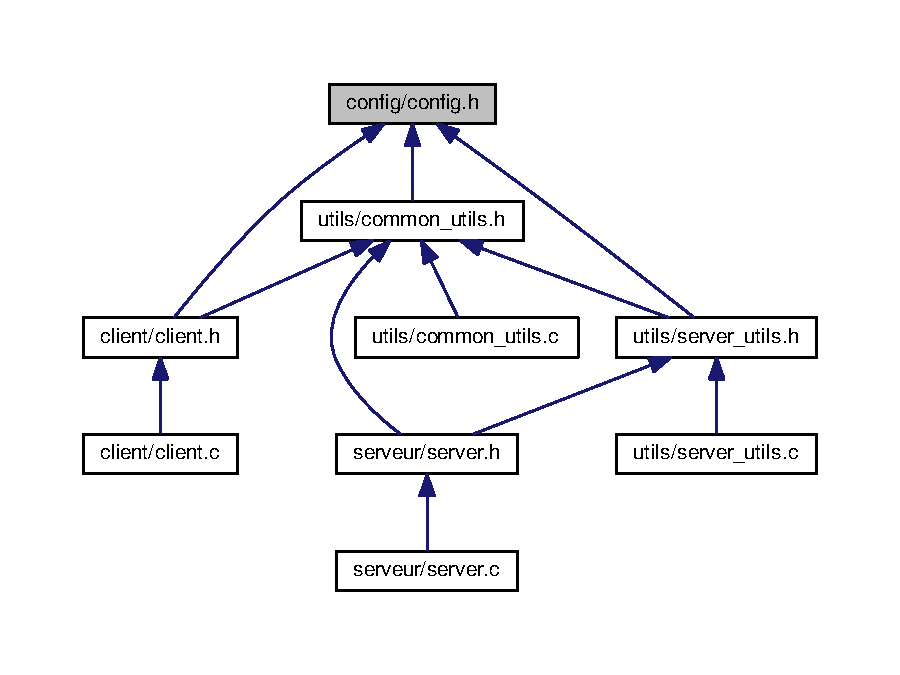
\includegraphics[width=350pt]{config_8h__dep__incl}
\end{center}
\end{figure}
\subsection*{Macros}
\begin{DoxyCompactItemize}
\item 
\#define \hyperlink{config_8h_aa8cecfc5c5c054d2875c03e77b7be15d}{T\+R\+UE}~1
\item 
\#define \hyperlink{config_8h_aa93f0eb578d23995850d61f7d61c55c1}{F\+A\+L\+SE}~0
\item 
\#define \hyperlink{config_8h_aef72fe86b7c60b1a86920496456edeac}{W\+A\+IT}~0
\item 
\#define \hyperlink{config_8h_acc47e9180a9dc8aafbd10fe6cfb8e336}{R\+E\+F\+U\+SE}~1
\item 
\#define \hyperlink{config_8h_a44ad8d0e0924a99b99a5a6a1aa776c33}{D\+E\+AL}~4
\item 
\#define \hyperlink{config_8h_a5e1a9330a996857d164653e4aba8fbfb}{A\+SK}~5
\item 
\#define \hyperlink{config_8h_abf70a4804c459727975816dd16613d45}{G\+I\+VE}~7
\item 
\#define \hyperlink{config_8h_af144c56be720021d0c3a8075b87ff9b5}{R\+O\+U\+ND}~9
\item 
\#define \hyperlink{config_8h_adc5ff46918e62c92962966a7ad4d2876}{S\+C\+O\+R\+ES}~11
\item 
\#define \hyperlink{config_8h_a148665c75ac246648923b90119015f88}{W\+I\+N\+N\+ER}~12
\item 
\#define \hyperlink{config_8h_a3e7bdaa0015ef87c8099040222f60f76}{D\+E\+F\+I\+N\+E\+\_\+\+C\+A\+RD}~13
\item 
\#define \hyperlink{config_8h_a013bea065579104a43f1bc426dae69aa}{N\+I\+C\+K\+N\+A\+ME}~2
\item 
\#define \hyperlink{config_8h_a34deddb3d2e1791fd7ce5acc13ffc8df}{P\+L\+AY}~6
\item 
\#define \hyperlink{config_8h_a2b7cf2a3641be7b89138615764d60ba3}{E\+M\+P\+TY}~8
\item 
\#define \hyperlink{config_8h_a00658ed53f1bd7b1ecc33f45de053171}{S\+C\+O\+RE}~10
\item 
\#define \hyperlink{config_8h_a587604e6f3570c0fc32794384d4d0d1f}{D\+I\+S\+C\+O\+N\+N\+E\+CT}~3
\item 
\#define \hyperlink{config_8h_a1725876d3b41d0601d59768e442b7907}{P\+O\+R\+T\+\_\+\+D\+I\+M\+OV}~17626
\item 
\#define \hyperlink{config_8h_a54e6973435c6c9667fd94f2fd967456c}{P\+O\+R\+T\+\_\+\+D\+R\+A\+G\+O\+M\+IR}~18206
\item 
\#define \hyperlink{config_8h_a1c346c944e8204fd06dc057393c7c96d}{M\+A\+X\+\_\+\+P\+L\+A\+Y\+E\+RS}~4
\item 
\#define \hyperlink{config_8h_ad79aefee6a8990632311a15e98d9a65f}{N\+A\+M\+E\+S\+I\+ZE}~20
\item 
\#define \hyperlink{config_8h_aeca90e1c1c62b70670514ffc18c9dfd4}{M\+E\+S\+S\+A\+G\+E\+\_\+\+S\+I\+ZE}~82
\item 
\#define \hyperlink{config_8h_a195eca3016b16705bcd6afcd503a1e74}{N\+I\+C\+K\+N\+A\+M\+E\+S\+\_\+\+K\+EY}~\char`\"{}nicknames\char`\"{}
\end{DoxyCompactItemize}
\subsection*{Typedefs}
\begin{DoxyCompactItemize}
\item 
typedef int \hyperlink{config_8h_a1062901a7428fdd9c7f180f5e01ea056}{bool}
\end{DoxyCompactItemize}


\subsection{Macro Definition Documentation}
\index{config.\+h@{config.\+h}!A\+SK@{A\+SK}}
\index{A\+SK@{A\+SK}!config.\+h@{config.\+h}}
\subsubsection[{\texorpdfstring{A\+SK}{ASK}}]{\setlength{\rightskip}{0pt plus 5cm}\#define A\+SK~5}\hypertarget{config_8h_a5e1a9330a996857d164653e4aba8fbfb}{}\label{config_8h_a5e1a9330a996857d164653e4aba8fbfb}
\index{config.\+h@{config.\+h}!D\+E\+AL@{D\+E\+AL}}
\index{D\+E\+AL@{D\+E\+AL}!config.\+h@{config.\+h}}
\subsubsection[{\texorpdfstring{D\+E\+AL}{DEAL}}]{\setlength{\rightskip}{0pt plus 5cm}\#define D\+E\+AL~4}\hypertarget{config_8h_a44ad8d0e0924a99b99a5a6a1aa776c33}{}\label{config_8h_a44ad8d0e0924a99b99a5a6a1aa776c33}
\index{config.\+h@{config.\+h}!D\+E\+F\+I\+N\+E\+\_\+\+C\+A\+RD@{D\+E\+F\+I\+N\+E\+\_\+\+C\+A\+RD}}
\index{D\+E\+F\+I\+N\+E\+\_\+\+C\+A\+RD@{D\+E\+F\+I\+N\+E\+\_\+\+C\+A\+RD}!config.\+h@{config.\+h}}
\subsubsection[{\texorpdfstring{D\+E\+F\+I\+N\+E\+\_\+\+C\+A\+RD}{DEFINE_CARD}}]{\setlength{\rightskip}{0pt plus 5cm}\#define D\+E\+F\+I\+N\+E\+\_\+\+C\+A\+RD~13}\hypertarget{config_8h_a3e7bdaa0015ef87c8099040222f60f76}{}\label{config_8h_a3e7bdaa0015ef87c8099040222f60f76}
\index{config.\+h@{config.\+h}!D\+I\+S\+C\+O\+N\+N\+E\+CT@{D\+I\+S\+C\+O\+N\+N\+E\+CT}}
\index{D\+I\+S\+C\+O\+N\+N\+E\+CT@{D\+I\+S\+C\+O\+N\+N\+E\+CT}!config.\+h@{config.\+h}}
\subsubsection[{\texorpdfstring{D\+I\+S\+C\+O\+N\+N\+E\+CT}{DISCONNECT}}]{\setlength{\rightskip}{0pt plus 5cm}\#define D\+I\+S\+C\+O\+N\+N\+E\+CT~3}\hypertarget{config_8h_a587604e6f3570c0fc32794384d4d0d1f}{}\label{config_8h_a587604e6f3570c0fc32794384d4d0d1f}
\index{config.\+h@{config.\+h}!E\+M\+P\+TY@{E\+M\+P\+TY}}
\index{E\+M\+P\+TY@{E\+M\+P\+TY}!config.\+h@{config.\+h}}
\subsubsection[{\texorpdfstring{E\+M\+P\+TY}{EMPTY}}]{\setlength{\rightskip}{0pt plus 5cm}\#define E\+M\+P\+TY~8}\hypertarget{config_8h_a2b7cf2a3641be7b89138615764d60ba3}{}\label{config_8h_a2b7cf2a3641be7b89138615764d60ba3}
\index{config.\+h@{config.\+h}!F\+A\+L\+SE@{F\+A\+L\+SE}}
\index{F\+A\+L\+SE@{F\+A\+L\+SE}!config.\+h@{config.\+h}}
\subsubsection[{\texorpdfstring{F\+A\+L\+SE}{FALSE}}]{\setlength{\rightskip}{0pt plus 5cm}\#define F\+A\+L\+SE~0}\hypertarget{config_8h_aa93f0eb578d23995850d61f7d61c55c1}{}\label{config_8h_aa93f0eb578d23995850d61f7d61c55c1}
\index{config.\+h@{config.\+h}!G\+I\+VE@{G\+I\+VE}}
\index{G\+I\+VE@{G\+I\+VE}!config.\+h@{config.\+h}}
\subsubsection[{\texorpdfstring{G\+I\+VE}{GIVE}}]{\setlength{\rightskip}{0pt plus 5cm}\#define G\+I\+VE~7}\hypertarget{config_8h_abf70a4804c459727975816dd16613d45}{}\label{config_8h_abf70a4804c459727975816dd16613d45}
\index{config.\+h@{config.\+h}!M\+A\+X\+\_\+\+P\+L\+A\+Y\+E\+RS@{M\+A\+X\+\_\+\+P\+L\+A\+Y\+E\+RS}}
\index{M\+A\+X\+\_\+\+P\+L\+A\+Y\+E\+RS@{M\+A\+X\+\_\+\+P\+L\+A\+Y\+E\+RS}!config.\+h@{config.\+h}}
\subsubsection[{\texorpdfstring{M\+A\+X\+\_\+\+P\+L\+A\+Y\+E\+RS}{MAX_PLAYERS}}]{\setlength{\rightskip}{0pt plus 5cm}\#define M\+A\+X\+\_\+\+P\+L\+A\+Y\+E\+RS~4}\hypertarget{config_8h_a1c346c944e8204fd06dc057393c7c96d}{}\label{config_8h_a1c346c944e8204fd06dc057393c7c96d}
\index{config.\+h@{config.\+h}!M\+E\+S\+S\+A\+G\+E\+\_\+\+S\+I\+ZE@{M\+E\+S\+S\+A\+G\+E\+\_\+\+S\+I\+ZE}}
\index{M\+E\+S\+S\+A\+G\+E\+\_\+\+S\+I\+ZE@{M\+E\+S\+S\+A\+G\+E\+\_\+\+S\+I\+ZE}!config.\+h@{config.\+h}}
\subsubsection[{\texorpdfstring{M\+E\+S\+S\+A\+G\+E\+\_\+\+S\+I\+ZE}{MESSAGE_SIZE}}]{\setlength{\rightskip}{0pt plus 5cm}\#define M\+E\+S\+S\+A\+G\+E\+\_\+\+S\+I\+ZE~82}\hypertarget{config_8h_aeca90e1c1c62b70670514ffc18c9dfd4}{}\label{config_8h_aeca90e1c1c62b70670514ffc18c9dfd4}
\index{config.\+h@{config.\+h}!N\+A\+M\+E\+S\+I\+ZE@{N\+A\+M\+E\+S\+I\+ZE}}
\index{N\+A\+M\+E\+S\+I\+ZE@{N\+A\+M\+E\+S\+I\+ZE}!config.\+h@{config.\+h}}
\subsubsection[{\texorpdfstring{N\+A\+M\+E\+S\+I\+ZE}{NAMESIZE}}]{\setlength{\rightskip}{0pt plus 5cm}\#define N\+A\+M\+E\+S\+I\+ZE~20}\hypertarget{config_8h_ad79aefee6a8990632311a15e98d9a65f}{}\label{config_8h_ad79aefee6a8990632311a15e98d9a65f}
\index{config.\+h@{config.\+h}!N\+I\+C\+K\+N\+A\+ME@{N\+I\+C\+K\+N\+A\+ME}}
\index{N\+I\+C\+K\+N\+A\+ME@{N\+I\+C\+K\+N\+A\+ME}!config.\+h@{config.\+h}}
\subsubsection[{\texorpdfstring{N\+I\+C\+K\+N\+A\+ME}{NICKNAME}}]{\setlength{\rightskip}{0pt plus 5cm}\#define N\+I\+C\+K\+N\+A\+ME~2}\hypertarget{config_8h_a013bea065579104a43f1bc426dae69aa}{}\label{config_8h_a013bea065579104a43f1bc426dae69aa}
\index{config.\+h@{config.\+h}!N\+I\+C\+K\+N\+A\+M\+E\+S\+\_\+\+K\+EY@{N\+I\+C\+K\+N\+A\+M\+E\+S\+\_\+\+K\+EY}}
\index{N\+I\+C\+K\+N\+A\+M\+E\+S\+\_\+\+K\+EY@{N\+I\+C\+K\+N\+A\+M\+E\+S\+\_\+\+K\+EY}!config.\+h@{config.\+h}}
\subsubsection[{\texorpdfstring{N\+I\+C\+K\+N\+A\+M\+E\+S\+\_\+\+K\+EY}{NICKNAMES_KEY}}]{\setlength{\rightskip}{0pt plus 5cm}\#define N\+I\+C\+K\+N\+A\+M\+E\+S\+\_\+\+K\+EY~\char`\"{}nicknames\char`\"{}}\hypertarget{config_8h_a195eca3016b16705bcd6afcd503a1e74}{}\label{config_8h_a195eca3016b16705bcd6afcd503a1e74}
\index{config.\+h@{config.\+h}!P\+L\+AY@{P\+L\+AY}}
\index{P\+L\+AY@{P\+L\+AY}!config.\+h@{config.\+h}}
\subsubsection[{\texorpdfstring{P\+L\+AY}{PLAY}}]{\setlength{\rightskip}{0pt plus 5cm}\#define P\+L\+AY~6}\hypertarget{config_8h_a34deddb3d2e1791fd7ce5acc13ffc8df}{}\label{config_8h_a34deddb3d2e1791fd7ce5acc13ffc8df}
\index{config.\+h@{config.\+h}!P\+O\+R\+T\+\_\+\+D\+I\+M\+OV@{P\+O\+R\+T\+\_\+\+D\+I\+M\+OV}}
\index{P\+O\+R\+T\+\_\+\+D\+I\+M\+OV@{P\+O\+R\+T\+\_\+\+D\+I\+M\+OV}!config.\+h@{config.\+h}}
\subsubsection[{\texorpdfstring{P\+O\+R\+T\+\_\+\+D\+I\+M\+OV}{PORT_DIMOV}}]{\setlength{\rightskip}{0pt plus 5cm}\#define P\+O\+R\+T\+\_\+\+D\+I\+M\+OV~17626}\hypertarget{config_8h_a1725876d3b41d0601d59768e442b7907}{}\label{config_8h_a1725876d3b41d0601d59768e442b7907}
\index{config.\+h@{config.\+h}!P\+O\+R\+T\+\_\+\+D\+R\+A\+G\+O\+M\+IR@{P\+O\+R\+T\+\_\+\+D\+R\+A\+G\+O\+M\+IR}}
\index{P\+O\+R\+T\+\_\+\+D\+R\+A\+G\+O\+M\+IR@{P\+O\+R\+T\+\_\+\+D\+R\+A\+G\+O\+M\+IR}!config.\+h@{config.\+h}}
\subsubsection[{\texorpdfstring{P\+O\+R\+T\+\_\+\+D\+R\+A\+G\+O\+M\+IR}{PORT_DRAGOMIR}}]{\setlength{\rightskip}{0pt plus 5cm}\#define P\+O\+R\+T\+\_\+\+D\+R\+A\+G\+O\+M\+IR~18206}\hypertarget{config_8h_a54e6973435c6c9667fd94f2fd967456c}{}\label{config_8h_a54e6973435c6c9667fd94f2fd967456c}
\index{config.\+h@{config.\+h}!R\+E\+F\+U\+SE@{R\+E\+F\+U\+SE}}
\index{R\+E\+F\+U\+SE@{R\+E\+F\+U\+SE}!config.\+h@{config.\+h}}
\subsubsection[{\texorpdfstring{R\+E\+F\+U\+SE}{REFUSE}}]{\setlength{\rightskip}{0pt plus 5cm}\#define R\+E\+F\+U\+SE~1}\hypertarget{config_8h_acc47e9180a9dc8aafbd10fe6cfb8e336}{}\label{config_8h_acc47e9180a9dc8aafbd10fe6cfb8e336}
\index{config.\+h@{config.\+h}!R\+O\+U\+ND@{R\+O\+U\+ND}}
\index{R\+O\+U\+ND@{R\+O\+U\+ND}!config.\+h@{config.\+h}}
\subsubsection[{\texorpdfstring{R\+O\+U\+ND}{ROUND}}]{\setlength{\rightskip}{0pt plus 5cm}\#define R\+O\+U\+ND~9}\hypertarget{config_8h_af144c56be720021d0c3a8075b87ff9b5}{}\label{config_8h_af144c56be720021d0c3a8075b87ff9b5}
\index{config.\+h@{config.\+h}!S\+C\+O\+RE@{S\+C\+O\+RE}}
\index{S\+C\+O\+RE@{S\+C\+O\+RE}!config.\+h@{config.\+h}}
\subsubsection[{\texorpdfstring{S\+C\+O\+RE}{SCORE}}]{\setlength{\rightskip}{0pt plus 5cm}\#define S\+C\+O\+RE~10}\hypertarget{config_8h_a00658ed53f1bd7b1ecc33f45de053171}{}\label{config_8h_a00658ed53f1bd7b1ecc33f45de053171}
\index{config.\+h@{config.\+h}!S\+C\+O\+R\+ES@{S\+C\+O\+R\+ES}}
\index{S\+C\+O\+R\+ES@{S\+C\+O\+R\+ES}!config.\+h@{config.\+h}}
\subsubsection[{\texorpdfstring{S\+C\+O\+R\+ES}{SCORES}}]{\setlength{\rightskip}{0pt plus 5cm}\#define S\+C\+O\+R\+ES~11}\hypertarget{config_8h_adc5ff46918e62c92962966a7ad4d2876}{}\label{config_8h_adc5ff46918e62c92962966a7ad4d2876}
\index{config.\+h@{config.\+h}!T\+R\+UE@{T\+R\+UE}}
\index{T\+R\+UE@{T\+R\+UE}!config.\+h@{config.\+h}}
\subsubsection[{\texorpdfstring{T\+R\+UE}{TRUE}}]{\setlength{\rightskip}{0pt plus 5cm}\#define T\+R\+UE~1}\hypertarget{config_8h_aa8cecfc5c5c054d2875c03e77b7be15d}{}\label{config_8h_aa8cecfc5c5c054d2875c03e77b7be15d}
\index{config.\+h@{config.\+h}!W\+A\+IT@{W\+A\+IT}}
\index{W\+A\+IT@{W\+A\+IT}!config.\+h@{config.\+h}}
\subsubsection[{\texorpdfstring{W\+A\+IT}{WAIT}}]{\setlength{\rightskip}{0pt plus 5cm}\#define W\+A\+IT~0}\hypertarget{config_8h_aef72fe86b7c60b1a86920496456edeac}{}\label{config_8h_aef72fe86b7c60b1a86920496456edeac}
\index{config.\+h@{config.\+h}!W\+I\+N\+N\+ER@{W\+I\+N\+N\+ER}}
\index{W\+I\+N\+N\+ER@{W\+I\+N\+N\+ER}!config.\+h@{config.\+h}}
\subsubsection[{\texorpdfstring{W\+I\+N\+N\+ER}{WINNER}}]{\setlength{\rightskip}{0pt plus 5cm}\#define W\+I\+N\+N\+ER~12}\hypertarget{config_8h_a148665c75ac246648923b90119015f88}{}\label{config_8h_a148665c75ac246648923b90119015f88}


\subsection{Typedef Documentation}
\index{config.\+h@{config.\+h}!bool@{bool}}
\index{bool@{bool}!config.\+h@{config.\+h}}
\subsubsection[{\texorpdfstring{bool}{bool}}]{\setlength{\rightskip}{0pt plus 5cm}typedef int {\bf bool}}\hypertarget{config_8h_a1062901a7428fdd9c7f180f5e01ea056}{}\label{config_8h_a1062901a7428fdd9c7f180f5e01ea056}

\hypertarget{ports_8h}{}\section{config/ports.h File Reference}
\label{ports_8h}\index{config/ports.\+h@{config/ports.\+h}}


Projet de M\+C\+S3 2016 2017.  


\subsection*{Macros}
\begin{DoxyCompactItemize}
\item 
\#define \hyperlink{ports_8h_a1725876d3b41d0601d59768e442b7907}{P\+O\+R\+T\+\_\+\+D\+I\+M\+OV}~17626
\item 
\#define \hyperlink{ports_8h_a54e6973435c6c9667fd94f2fd967456c}{P\+O\+R\+T\+\_\+\+D\+R\+A\+G\+O\+M\+IR}~18206
\end{DoxyCompactItemize}


\subsection{Detailed Description}
Projet de M\+C\+S3 2016 2017. 

\begin{DoxyAuthor}{Author}
B\+E\+N\+C\+H\+I\+HA -\/ S\+A\+L\+E\+N\+G\+RO -\/ L\+E\+F\+O\+RT 
\end{DoxyAuthor}
\begin{DoxyVersion}{Version}
1 
\end{DoxyVersion}
\begin{DoxyDate}{Date}
D\+E\+C\+E\+M\+B\+RE -\/ J\+A\+N\+V\+I\+ER
\end{DoxyDate}
Fichier header des ports 

\subsection{Macro Definition Documentation}
\index{ports.\+h@{ports.\+h}!P\+O\+R\+T\+\_\+\+D\+I\+M\+OV@{P\+O\+R\+T\+\_\+\+D\+I\+M\+OV}}
\index{P\+O\+R\+T\+\_\+\+D\+I\+M\+OV@{P\+O\+R\+T\+\_\+\+D\+I\+M\+OV}!ports.\+h@{ports.\+h}}
\subsubsection[{\texorpdfstring{P\+O\+R\+T\+\_\+\+D\+I\+M\+OV}{PORT_DIMOV}}]{\setlength{\rightskip}{0pt plus 5cm}\#define P\+O\+R\+T\+\_\+\+D\+I\+M\+OV~17626}\hypertarget{ports_8h_a1725876d3b41d0601d59768e442b7907}{}\label{ports_8h_a1725876d3b41d0601d59768e442b7907}
\index{ports.\+h@{ports.\+h}!P\+O\+R\+T\+\_\+\+D\+R\+A\+G\+O\+M\+IR@{P\+O\+R\+T\+\_\+\+D\+R\+A\+G\+O\+M\+IR}}
\index{P\+O\+R\+T\+\_\+\+D\+R\+A\+G\+O\+M\+IR@{P\+O\+R\+T\+\_\+\+D\+R\+A\+G\+O\+M\+IR}!ports.\+h@{ports.\+h}}
\subsubsection[{\texorpdfstring{P\+O\+R\+T\+\_\+\+D\+R\+A\+G\+O\+M\+IR}{PORT_DRAGOMIR}}]{\setlength{\rightskip}{0pt plus 5cm}\#define P\+O\+R\+T\+\_\+\+D\+R\+A\+G\+O\+M\+IR~18206}\hypertarget{ports_8h_a54e6973435c6c9667fd94f2fd967456c}{}\label{ports_8h_a54e6973435c6c9667fd94f2fd967456c}

\hypertarget{server_8c}{}\section{serveur/server.c File Reference}
\label{server_8c}\index{serveur/server.\+c@{serveur/server.\+c}}


Projet de M\+C\+S3 2016 2017.  


{\ttfamily \#include \char`\"{}server.\+h\char`\"{}}\\*
Include dependency graph for server.\+c\+:
\nopagebreak
\begin{figure}[H]
\begin{center}
\leavevmode
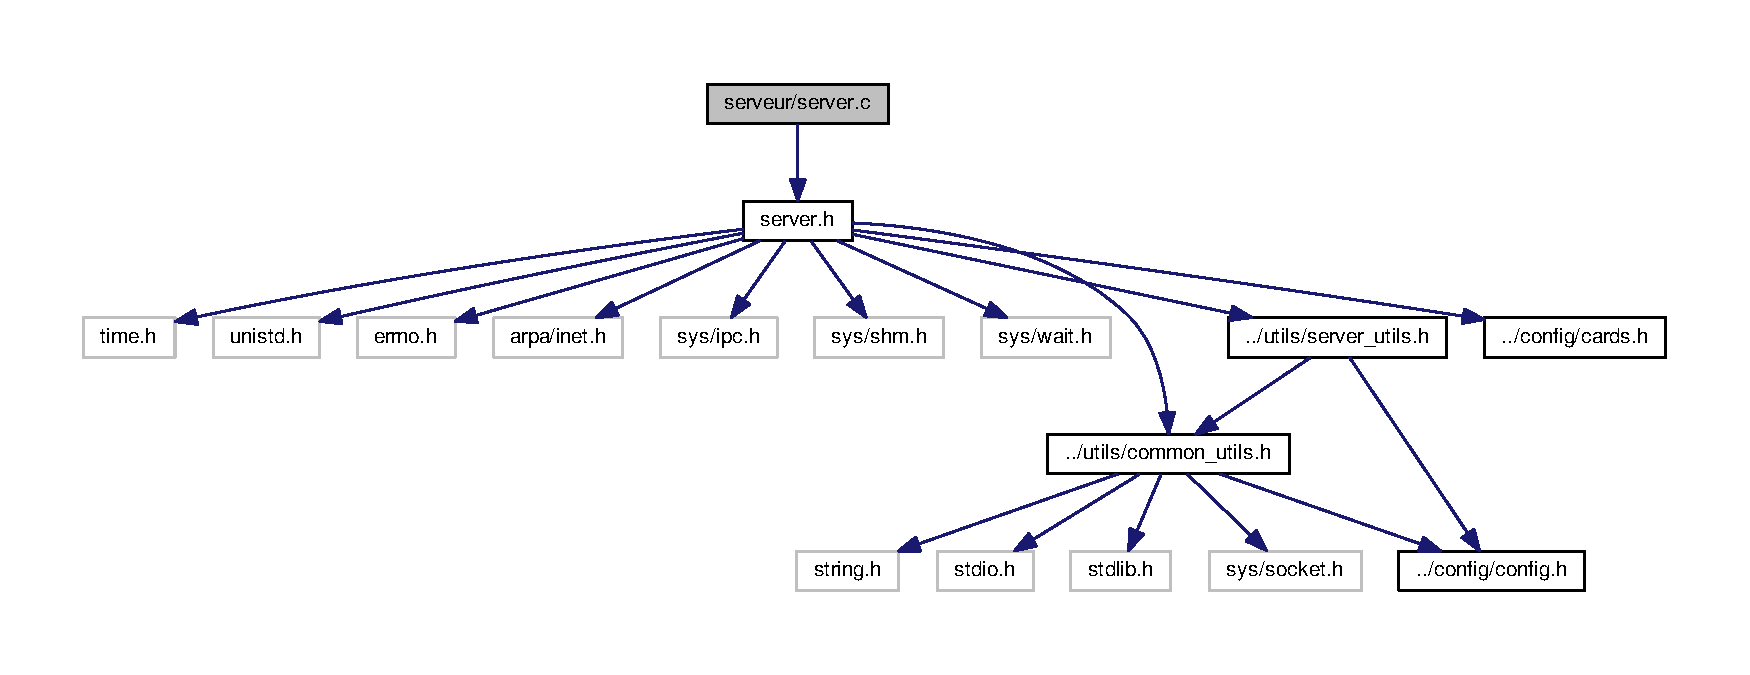
\includegraphics[width=350pt]{server_8c__incl}
\end{center}
\end{figure}
\subsection*{Functions}
\begin{DoxyCompactItemize}
\item 
int \hyperlink{server_8c_a3c04138a5bfe5d72780bb7e82a18e627}{main} (int argc, char $\ast$$\ast$argv)
\item 
void \hyperlink{server_8c_a6745b86fbd6eeec00e183b7fffe894e8}{alarm\+\_\+handler} (int signum)
\begin{DoxyCompactList}\small\item\em Fonction signal qui regarde s\textquotesingle{}il y a au moins deux joueurs. Sinon ça quitte le jeu. \end{DoxyCompactList}\item 
int \hyperlink{server_8c_a9e7dde7473d44f17f66d5e731b74664b}{find\+\_\+index} (\hyperlink{structplayer}{player} $\ast$\hyperlink{server_8c_ae6858c39ad2db341164105c6e73ba927}{joueurs}, int socket)
\begin{DoxyCompactList}\small\item\em Fonction d\textquotesingle{}indexage des joueurs. \end{DoxyCompactList}\item 
void \hyperlink{server_8c_a1e135d989cd28349169939c6a73f2e87}{interrupt\+\_\+handler} (int signum)
\begin{DoxyCompactList}\small\item\em Fonction de déconnexion d\textquotesingle{}un client suita à un controle C. \end{DoxyCompactList}\item 
void \hyperlink{server_8c_a959e96ab48f9d10f26bd477875f25085}{init\+\_\+server} (int $\ast$server\+\_\+socket, struct sockaddr\+\_\+in $\ast$my\+\_\+addr)
\begin{DoxyCompactList}\small\item\em Fonction d\textquotesingle{}initialisation du serveur. \end{DoxyCompactList}\item 
void \hyperlink{server_8c_a9c4135e5c61f79ef065e3938bab962bf}{add\+\_\+client} (int server\+\_\+socket, struct sockaddr\+\_\+in $\ast$cl\+\_\+addr)
\begin{DoxyCompactList}\small\item\em Fonction d\textquotesingle{}ajout d\textquotesingle{}un client au serveur. Si le jeu est en cours, on refuse la connexion S\textquotesingle{}il y a 4 personnes on ferme le lobby. \end{DoxyCompactList}\item 
void \hyperlink{server_8c_ad24f7f5e3ba657d640f0b4a251c89dfc}{add\+\_\+player} (int socket)
\begin{DoxyCompactList}\small\item\em Fonction qio ajoute un joueur. \end{DoxyCompactList}\item 
void \hyperlink{server_8c_a4202fa5c5191c7e387d7570da6c8cd8c}{end\+\_\+game} ()
\begin{DoxyCompactList}\small\item\em Fonction de fin de jeu. \end{DoxyCompactList}\item 
void \hyperlink{server_8c_af6a4c4855466fbe111b571c32c4d85df}{remove\+\_\+player} (\hyperlink{structplayer}{player} $\ast$\hyperlink{server_8c_ae6858c39ad2db341164105c6e73ba927}{joueurs}, int index, \hyperlink{config_8h_a1062901a7428fdd9c7f180f5e01ea056}{bool} sockopen)
\begin{DoxyCompactList}\small\item\em Fonction qui retire un joueur. \end{DoxyCompactList}\item 
void \hyperlink{server_8c_a5e9451e44b0f186c7fe17bbc0dcd7945}{refuse\+\_\+connection} (int socket)
\begin{DoxyCompactList}\small\item\em Fonction de refus de connexion. Envoie d\textquotesingle{}un message avec le code R\+E\+F\+US défini dans \hyperlink{config_8h}{config.\+h}. \end{DoxyCompactList}\item 
void \hyperlink{server_8c_a459871e1c13a57040170a8b3eb5f0a05}{add\+\_\+nickname} (int socket, char $\ast$$\ast$msg)
\begin{DoxyCompactList}\small\item\em Fonction qui ajoute le pseudo de 20 char max. \end{DoxyCompactList}\item 
void \hyperlink{server_8c_a528ee6cf05cb3b1af23306dc055e5eb3}{deal\+\_\+cards} ()
\begin{DoxyCompactList}\small\item\em Fonction de distribution des cartes. \end{DoxyCompactList}\item 
void \hyperlink{server_8c_aa6808a03a0851a7d5290d8c281ccbb9f}{clear\+\_\+lobby} ()
\begin{DoxyCompactList}\small\item\em Fonction de nettoyage du lobby après qu\textquotesingle{}un joueur ait quitté le salon. \end{DoxyCompactList}\item 
\hyperlink{config_8h_a1062901a7428fdd9c7f180f5e01ea056}{bool} \hyperlink{server_8c_aa00c65085c2cd2397e9ff7fa70b06a4e}{receive\+\_\+msg} (char $\ast$msg, int fd)
\begin{DoxyCompactList}\small\item\em Fonction de Récception de message du serveur. \end{DoxyCompactList}\item 
void \hyperlink{server_8c_a671b58f5509a3a9fa692bacccfc32cc9}{start\+\_\+game} ()
\begin{DoxyCompactList}\small\item\em Fonction qui met le jeu en marche. Du coup, le jeu est en statut \+: \char`\"{}\+En cours\char`\"{}. \end{DoxyCompactList}\item 
void \hyperlink{server_8c_ac81d67cd3689820d5a77d7a302a69e5c}{start\+\_\+round} ()
\begin{DoxyCompactList}\small\item\em Fonction de démarrage du round. \end{DoxyCompactList}\item 
void \hyperlink{server_8c_aa19a1bc56fc2328f643ee05d28207005}{shutdown\+\_\+socket} (int socket)
\begin{DoxyCompactList}\small\item\em Fonction de fermeture de la socket. \end{DoxyCompactList}\item 
void \hyperlink{server_8c_a823119f7fbe44e03c0d173e74a595a0b}{shutdown\+\_\+server} ()
\begin{DoxyCompactList}\small\item\em Fonction de fermeture du serveur. \end{DoxyCompactList}\item 
void \hyperlink{server_8c_aa23110807cc8a40926f3a3774c4a9d8c}{receive\+\_\+card} (int socket, char $\ast$$\ast$msg)
\begin{DoxyCompactList}\small\item\em Fonction de réception des cartes. \end{DoxyCompactList}\item 
void \hyperlink{server_8c_a02e51511a0484dc245b85e1203a6bca2}{end\+\_\+round} (int socket, char $\ast$$\ast$msg)
\begin{DoxyCompactList}\small\item\em Fonction terminer un round. \end{DoxyCompactList}\item 
void \hyperlink{server_8c_a52c10f930760467c51180b598ec79d2b}{update\+\_\+score} (int socket, char $\ast$$\ast$msg)
\begin{DoxyCompactList}\small\item\em Fonction de mise à jour du score. \end{DoxyCompactList}\end{DoxyCompactItemize}
\subsection*{Variables}
\begin{DoxyCompactItemize}
\item 
int \hyperlink{server_8c_ae7b035800c3d74b46fa90a7351257843}{cl\+\_\+count}
\item 
int \hyperlink{server_8c_a664e80fb5c82f277c9b0b854f57448d9}{scores\+\_\+joueurs} \mbox{[}\hyperlink{config_8h_a1c346c944e8204fd06dc057393c7c96d}{M\+A\+X\+\_\+\+P\+L\+A\+Y\+E\+RS}\mbox{]}
\item 
\hyperlink{structplayer}{player} \hyperlink{server_8c_ae6858c39ad2db341164105c6e73ba927}{joueurs} \mbox{[}\hyperlink{config_8h_a1c346c944e8204fd06dc057393c7c96d}{M\+A\+X\+\_\+\+P\+L\+A\+Y\+E\+RS}\mbox{]}
\item 
\hyperlink{config_8h_a1062901a7428fdd9c7f180f5e01ea056}{bool} \hyperlink{server_8c_a5ed30d894bdb772c33f17e1475c09cde}{jeu\+\_\+en\+\_\+cours}
\item 
\hyperlink{config_8h_a1062901a7428fdd9c7f180f5e01ea056}{bool} \hyperlink{server_8c_a67e9cc16552fbd0741cd873b72984048}{temps\+\_\+termine}
\item 
\hyperlink{config_8h_a1062901a7428fdd9c7f180f5e01ea056}{bool} \hyperlink{server_8c_a69f52927a2dc43f5db4c13fc565a7498}{serveur\+\_\+en\+\_\+cours}
\item 
\hyperlink{config_8h_a1062901a7428fdd9c7f180f5e01ea056}{bool} \hyperlink{server_8c_ae14734f17ec04f911a0a8dc60c21fa87}{fin\+\_\+du\+\_\+tour}
\item 
\hyperlink{config_8h_a1062901a7428fdd9c7f180f5e01ea056}{bool} \hyperlink{server_8c_a9116f217b2e7ccc18feca002336eba7f}{sigempty}
\item 
\hyperlink{config_8h_a1062901a7428fdd9c7f180f5e01ea056}{bool} \hyperlink{server_8c_a1adc734d4ffd0ac2528f57dd97384b8c}{fin\+\_\+du\+\_\+round}
\item 
\hyperlink{server_8h_a6b8fa7d1c828463f6e6650a7dbc743e3}{fct\+\_\+ptr} \hyperlink{server_8c_ad39f0d9f3baee2caf8632acc84535397}{dispatcher} \mbox{[}$\,$\mbox{]} = \{ \hyperlink{server_8h_aa694be34287e456e5e22f60cedd022e5}{add\+\_\+player}, \hyperlink{server_8h_a70b88da842b28ecee8ce334b84d1a9fa}{refuse\+\_\+connection}, \hyperlink{server_8h_a586579926dbdc1e0c4b4fcecd2eacb7b}{add\+\_\+nickname}, 0, 0, 0, \hyperlink{server_8h_a0aba0f88abe71a413343d35ee5995683}{receive\+\_\+card}, 0, \hyperlink{server_8h_a26877a4a2039828bb05743dce8916132}{end\+\_\+round}, 0, \hyperlink{server_8h_afbb3dc95041fa32e01347ab80cc8c0fb}{update\+\_\+score} \}
\end{DoxyCompactItemize}


\subsection{Detailed Description}
Projet de M\+C\+S3 2016 2017. 

\begin{DoxyAuthor}{Author}
B\+E\+N\+C\+H\+I\+HA -\/ S\+A\+L\+E\+N\+G\+RO -\/ L\+E\+F\+O\+RT 
\end{DoxyAuthor}
\begin{DoxyVersion}{Version}
1 
\end{DoxyVersion}
\begin{DoxyDate}{Date}
D\+E\+C\+E\+M\+B\+RE -\/ J\+A\+N\+V\+I\+ER Fichier gérant les constantes propore au jeu
\end{DoxyDate}
\begin{DoxyAuthor}{Author}
B\+E\+N\+C\+H\+I\+HA -\/ S\+A\+L\+E\+N\+G\+RO -\/ L\+E\+F\+O\+RT 
\end{DoxyAuthor}
\begin{DoxyVersion}{Version}
1 
\end{DoxyVersion}
\begin{DoxyDate}{Date}
D\+E\+C\+E\+M\+B\+RE -\/ J\+A\+N\+V\+I\+ER
\end{DoxyDate}
Fichier gérant le serveur du projet 

\subsection{Function Documentation}
\index{server.\+c@{server.\+c}!add\+\_\+client@{add\+\_\+client}}
\index{add\+\_\+client@{add\+\_\+client}!server.\+c@{server.\+c}}
\subsubsection[{\texorpdfstring{add\+\_\+client(int server\+\_\+socket, struct sockaddr\+\_\+in $\ast$cl\+\_\+addr)}{add_client(int server_socket, struct sockaddr_in *cl_addr)}}]{\setlength{\rightskip}{0pt plus 5cm}add\+\_\+client (
\begin{DoxyParamCaption}
\item[{int}]{server\+\_\+socket, }
\item[{struct sockaddr\+\_\+in $\ast$}]{cl\+\_\+addr}
\end{DoxyParamCaption}
)}\hypertarget{server_8c_a9c4135e5c61f79ef065e3938bab962bf}{}\label{server_8c_a9c4135e5c61f79ef065e3938bab962bf}


Fonction d\textquotesingle{}ajout d\textquotesingle{}un client au serveur. Si le jeu est en cours, on refuse la connexion S\textquotesingle{}il y a 4 personnes on ferme le lobby. 


\begin{DoxyParams}{Parameters}
{\em server\+\_\+socket} & \\
\hline
{\em $\ast$cl\+\_\+addr} & \\
\hline
\end{DoxyParams}
\begin{DoxyReturn}{Returns}
V\+O\+ID 
\end{DoxyReturn}
\index{server.\+c@{server.\+c}!add\+\_\+nickname@{add\+\_\+nickname}}
\index{add\+\_\+nickname@{add\+\_\+nickname}!server.\+c@{server.\+c}}
\subsubsection[{\texorpdfstring{add\+\_\+nickname(int socket, char $\ast$$\ast$msg)}{add_nickname(int socket, char **msg)}}]{\setlength{\rightskip}{0pt plus 5cm}void add\+\_\+nickname (
\begin{DoxyParamCaption}
\item[{int}]{socket, }
\item[{char $\ast$$\ast$}]{msg}
\end{DoxyParamCaption}
)}\hypertarget{server_8c_a459871e1c13a57040170a8b3eb5f0a05}{}\label{server_8c_a459871e1c13a57040170a8b3eb5f0a05}


Fonction qui ajoute le pseudo de 20 char max. 


\begin{DoxyParams}{Parameters}
{\em socket} & \\
\hline
{\em $\ast$$\ast$msg} & \\
\hline
\end{DoxyParams}
\begin{DoxyReturn}{Returns}
V\+O\+ID 
\end{DoxyReturn}
\index{server.\+c@{server.\+c}!add\+\_\+player@{add\+\_\+player}}
\index{add\+\_\+player@{add\+\_\+player}!server.\+c@{server.\+c}}
\subsubsection[{\texorpdfstring{add\+\_\+player(int socket)}{add_player(int socket)}}]{\setlength{\rightskip}{0pt plus 5cm}void add\+\_\+player (
\begin{DoxyParamCaption}
\item[{int}]{socket}
\end{DoxyParamCaption}
)}\hypertarget{server_8c_ad24f7f5e3ba657d640f0b4a251c89dfc}{}\label{server_8c_ad24f7f5e3ba657d640f0b4a251c89dfc}


Fonction qio ajoute un joueur. 


\begin{DoxyParams}{Parameters}
{\em socket} & \\
\hline
\end{DoxyParams}
\begin{DoxyReturn}{Returns}
V\+O\+ID 
\end{DoxyReturn}
\index{server.\+c@{server.\+c}!alarm\+\_\+handler@{alarm\+\_\+handler}}
\index{alarm\+\_\+handler@{alarm\+\_\+handler}!server.\+c@{server.\+c}}
\subsubsection[{\texorpdfstring{alarm\+\_\+handler(int signum)}{alarm_handler(int signum)}}]{\setlength{\rightskip}{0pt plus 5cm}void alarm\+\_\+handler (
\begin{DoxyParamCaption}
\item[{int}]{signum}
\end{DoxyParamCaption}
)}\hypertarget{server_8c_a6745b86fbd6eeec00e183b7fffe894e8}{}\label{server_8c_a6745b86fbd6eeec00e183b7fffe894e8}


Fonction signal qui regarde s\textquotesingle{}il y a au moins deux joueurs. Sinon ça quitte le jeu. 


\begin{DoxyParams}{Parameters}
{\em signum} & numéro du signal \\
\hline
\end{DoxyParams}
\begin{DoxyReturn}{Returns}
V\+O\+ID 
\end{DoxyReturn}
\index{server.\+c@{server.\+c}!clear\+\_\+lobby@{clear\+\_\+lobby}}
\index{clear\+\_\+lobby@{clear\+\_\+lobby}!server.\+c@{server.\+c}}
\subsubsection[{\texorpdfstring{clear\+\_\+lobby()}{clear_lobby()}}]{\setlength{\rightskip}{0pt plus 5cm}clear\+\_\+lobby (
\begin{DoxyParamCaption}
{}
\end{DoxyParamCaption}
)}\hypertarget{server_8c_aa6808a03a0851a7d5290d8c281ccbb9f}{}\label{server_8c_aa6808a03a0851a7d5290d8c281ccbb9f}


Fonction de nettoyage du lobby après qu\textquotesingle{}un joueur ait quitté le salon. 


\begin{DoxyParams}{Parameters}
{\em V\+O\+ID} & \\
\hline
\end{DoxyParams}
\begin{DoxyReturn}{Returns}
V\+O\+ID 
\end{DoxyReturn}
\index{server.\+c@{server.\+c}!deal\+\_\+cards@{deal\+\_\+cards}}
\index{deal\+\_\+cards@{deal\+\_\+cards}!server.\+c@{server.\+c}}
\subsubsection[{\texorpdfstring{deal\+\_\+cards()}{deal_cards()}}]{\setlength{\rightskip}{0pt plus 5cm}void deal\+\_\+cards (
\begin{DoxyParamCaption}
{}
\end{DoxyParamCaption}
)}\hypertarget{server_8c_a528ee6cf05cb3b1af23306dc055e5eb3}{}\label{server_8c_a528ee6cf05cb3b1af23306dc055e5eb3}


Fonction de distribution des cartes. 


\begin{DoxyParams}{Parameters}
{\em void} & \\
\hline
\end{DoxyParams}
\begin{DoxyReturn}{Returns}
V\+O\+ID 
\end{DoxyReturn}
\index{server.\+c@{server.\+c}!end\+\_\+game@{end\+\_\+game}}
\index{end\+\_\+game@{end\+\_\+game}!server.\+c@{server.\+c}}
\subsubsection[{\texorpdfstring{end\+\_\+game()}{end_game()}}]{\setlength{\rightskip}{0pt plus 5cm}void end\+\_\+game (
\begin{DoxyParamCaption}
{}
\end{DoxyParamCaption}
)}\hypertarget{server_8c_a4202fa5c5191c7e387d7570da6c8cd8c}{}\label{server_8c_a4202fa5c5191c7e387d7570da6c8cd8c}


Fonction de fin de jeu. 


\begin{DoxyParams}{Parameters}
{\em information} & boolean qui va vérifier si on s\textquotesingle{}est déconnecté ou pas. \\
\hline
\end{DoxyParams}
\begin{DoxyReturn}{Returns}
V\+O\+ID 
\end{DoxyReturn}
\index{server.\+c@{server.\+c}!end\+\_\+round@{end\+\_\+round}}
\index{end\+\_\+round@{end\+\_\+round}!server.\+c@{server.\+c}}
\subsubsection[{\texorpdfstring{end\+\_\+round(int socket, char $\ast$$\ast$msg)}{end_round(int socket, char **msg)}}]{\setlength{\rightskip}{0pt plus 5cm}end\+\_\+round (
\begin{DoxyParamCaption}
\item[{int}]{socket, }
\item[{char $\ast$$\ast$}]{msg}
\end{DoxyParamCaption}
)}\hypertarget{server_8c_a02e51511a0484dc245b85e1203a6bca2}{}\label{server_8c_a02e51511a0484dc245b85e1203a6bca2}


Fonction terminer un round. 


\begin{DoxyParams}{Parameters}
{\em socket} & \\
\hline
{\em $\ast$$\ast$msg} & \\
\hline
\end{DoxyParams}
\begin{DoxyReturn}{Returns}
V\+O\+ID 
\end{DoxyReturn}
\index{server.\+c@{server.\+c}!find\+\_\+index@{find\+\_\+index}}
\index{find\+\_\+index@{find\+\_\+index}!server.\+c@{server.\+c}}
\subsubsection[{\texorpdfstring{find\+\_\+index(player $\ast$joueurs, int socket)}{find_index(player *joueurs, int socket)}}]{\setlength{\rightskip}{0pt plus 5cm}int find\+\_\+index (
\begin{DoxyParamCaption}
\item[{{\bf player} $\ast$}]{joueurs, }
\item[{int}]{socket}
\end{DoxyParamCaption}
)}\hypertarget{server_8c_a9e7dde7473d44f17f66d5e731b74664b}{}\label{server_8c_a9e7dde7473d44f17f66d5e731b74664b}


Fonction d\textquotesingle{}indexage des joueurs. 


\begin{DoxyParams}{Parameters}
{\em joueurs} & structure de données défini dans \hyperlink{server__utils_8h}{server\+\_\+utils.\+h} \\
\hline
{\em socket} & \\
\hline
\end{DoxyParams}
\begin{DoxyReturn}{Returns}
int 
\end{DoxyReturn}
\index{server.\+c@{server.\+c}!init\+\_\+server@{init\+\_\+server}}
\index{init\+\_\+server@{init\+\_\+server}!server.\+c@{server.\+c}}
\subsubsection[{\texorpdfstring{init\+\_\+server(int $\ast$server\+\_\+socket, struct sockaddr\+\_\+in $\ast$my\+\_\+addr)}{init_server(int *server_socket, struct sockaddr_in *my_addr)}}]{\setlength{\rightskip}{0pt plus 5cm}void init\+\_\+server (
\begin{DoxyParamCaption}
\item[{int $\ast$}]{server\+\_\+socket, }
\item[{struct sockaddr\+\_\+in $\ast$}]{my\+\_\+addr}
\end{DoxyParamCaption}
)}\hypertarget{server_8c_a959e96ab48f9d10f26bd477875f25085}{}\label{server_8c_a959e96ab48f9d10f26bd477875f25085}


Fonction d\textquotesingle{}initialisation du serveur. 


\begin{DoxyParams}{Parameters}
{\em $\ast$server\+\_\+socket} & \\
\hline
{\em $\ast$my\+\_\+addr} & \\
\hline
\end{DoxyParams}
\begin{DoxyReturn}{Returns}
V\+O\+ID 
\end{DoxyReturn}
\index{server.\+c@{server.\+c}!interrupt\+\_\+handler@{interrupt\+\_\+handler}}
\index{interrupt\+\_\+handler@{interrupt\+\_\+handler}!server.\+c@{server.\+c}}
\subsubsection[{\texorpdfstring{interrupt\+\_\+handler(int signum)}{interrupt_handler(int signum)}}]{\setlength{\rightskip}{0pt plus 5cm}void interrupt\+\_\+handler (
\begin{DoxyParamCaption}
\item[{int}]{signum}
\end{DoxyParamCaption}
)}\hypertarget{server_8c_a1e135d989cd28349169939c6a73f2e87}{}\label{server_8c_a1e135d989cd28349169939c6a73f2e87}


Fonction de déconnexion d\textquotesingle{}un client suita à un controle C. 

Fonction de signal d\textquotesingle{}interruption.


\begin{DoxyParams}{Parameters}
{\em signum} & signal vérifiant le controle C \\
\hline
\end{DoxyParams}
\begin{DoxyReturn}{Returns}
V\+O\+ID.
\end{DoxyReturn}

\begin{DoxyParams}{Parameters}
{\em signum} & \\
\hline
\end{DoxyParams}
\begin{DoxyReturn}{Returns}
V\+O\+ID 
\end{DoxyReturn}
\index{server.\+c@{server.\+c}!main@{main}}
\index{main@{main}!server.\+c@{server.\+c}}
\subsubsection[{\texorpdfstring{main(int argc, char $\ast$$\ast$argv)}{main(int argc, char **argv)}}]{\setlength{\rightskip}{0pt plus 5cm}int main (
\begin{DoxyParamCaption}
\item[{int}]{argc, }
\item[{char $\ast$$\ast$}]{argv}
\end{DoxyParamCaption}
)}\hypertarget{server_8c_a3c04138a5bfe5d72780bb7e82a18e627}{}\label{server_8c_a3c04138a5bfe5d72780bb7e82a18e627}
\index{server.\+c@{server.\+c}!receive\+\_\+card@{receive\+\_\+card}}
\index{receive\+\_\+card@{receive\+\_\+card}!server.\+c@{server.\+c}}
\subsubsection[{\texorpdfstring{receive\+\_\+card(int socket, char $\ast$$\ast$msg)}{receive_card(int socket, char **msg)}}]{\setlength{\rightskip}{0pt plus 5cm}void receive\+\_\+card (
\begin{DoxyParamCaption}
\item[{int}]{socket, }
\item[{char $\ast$$\ast$}]{msg}
\end{DoxyParamCaption}
)}\hypertarget{server_8c_aa23110807cc8a40926f3a3774c4a9d8c}{}\label{server_8c_aa23110807cc8a40926f3a3774c4a9d8c}


Fonction de réception des cartes. 


\begin{DoxyParams}{Parameters}
{\em socket} & \\
\hline
{\em $\ast$$\ast$msg} & \\
\hline
\end{DoxyParams}
\begin{DoxyReturn}{Returns}
V\+O\+ID 
\end{DoxyReturn}
\index{server.\+c@{server.\+c}!receive\+\_\+msg@{receive\+\_\+msg}}
\index{receive\+\_\+msg@{receive\+\_\+msg}!server.\+c@{server.\+c}}
\subsubsection[{\texorpdfstring{receive\+\_\+msg(char $\ast$msg, int fd)}{receive_msg(char *msg, int fd)}}]{\setlength{\rightskip}{0pt plus 5cm}{\bf bool} receive\+\_\+msg (
\begin{DoxyParamCaption}
\item[{char $\ast$}]{msg, }
\item[{int}]{fd}
\end{DoxyParamCaption}
)}\hypertarget{server_8c_aa00c65085c2cd2397e9ff7fa70b06a4e}{}\label{server_8c_aa00c65085c2cd2397e9ff7fa70b06a4e}


Fonction de Récception de message du serveur. 


\begin{DoxyParams}{Parameters}
{\em $\ast$msg} & \\
\hline
{\em fd} & \\
\hline
\end{DoxyParams}
\begin{DoxyReturn}{Returns}
bool 
\end{DoxyReturn}
\index{server.\+c@{server.\+c}!refuse\+\_\+connection@{refuse\+\_\+connection}}
\index{refuse\+\_\+connection@{refuse\+\_\+connection}!server.\+c@{server.\+c}}
\subsubsection[{\texorpdfstring{refuse\+\_\+connection(int socket)}{refuse_connection(int socket)}}]{\setlength{\rightskip}{0pt plus 5cm}void refuse\+\_\+connection (
\begin{DoxyParamCaption}
\item[{int}]{socket}
\end{DoxyParamCaption}
)}\hypertarget{server_8c_a5e9451e44b0f186c7fe17bbc0dcd7945}{}\label{server_8c_a5e9451e44b0f186c7fe17bbc0dcd7945}


Fonction de refus de connexion. Envoie d\textquotesingle{}un message avec le code R\+E\+F\+US défini dans \hyperlink{config_8h}{config.\+h}. 


\begin{DoxyParams}{Parameters}
{\em socket} & \\
\hline
\end{DoxyParams}
\begin{DoxyReturn}{Returns}
V\+O\+ID 
\end{DoxyReturn}
\index{server.\+c@{server.\+c}!remove\+\_\+player@{remove\+\_\+player}}
\index{remove\+\_\+player@{remove\+\_\+player}!server.\+c@{server.\+c}}
\subsubsection[{\texorpdfstring{remove\+\_\+player(player $\ast$joueurs, int index, bool sockopen)}{remove_player(player *joueurs, int index, bool sockopen)}}]{\setlength{\rightskip}{0pt plus 5cm}void remove\+\_\+player (
\begin{DoxyParamCaption}
\item[{{\bf player} $\ast$}]{joueurs, }
\item[{int}]{index, }
\item[{{\bf bool}}]{sockopen}
\end{DoxyParamCaption}
)}\hypertarget{server_8c_af6a4c4855466fbe111b571c32c4d85df}{}\label{server_8c_af6a4c4855466fbe111b571c32c4d85df}


Fonction qui retire un joueur. 


\begin{DoxyParams}{Parameters}
{\em joueur} & \\
\hline
{\em index} & \\
\hline
{\em sockopen} & \\
\hline
\end{DoxyParams}
\begin{DoxyReturn}{Returns}
V\+O\+ID 
\end{DoxyReturn}
\index{server.\+c@{server.\+c}!shutdown\+\_\+server@{shutdown\+\_\+server}}
\index{shutdown\+\_\+server@{shutdown\+\_\+server}!server.\+c@{server.\+c}}
\subsubsection[{\texorpdfstring{shutdown\+\_\+server()}{shutdown_server()}}]{\setlength{\rightskip}{0pt plus 5cm}void shutdown\+\_\+server (
\begin{DoxyParamCaption}
{}
\end{DoxyParamCaption}
)}\hypertarget{server_8c_a823119f7fbe44e03c0d173e74a595a0b}{}\label{server_8c_a823119f7fbe44e03c0d173e74a595a0b}


Fonction de fermeture du serveur. 


\begin{DoxyParams}{Parameters}
{\em void} & \\
\hline
\end{DoxyParams}
\begin{DoxyReturn}{Returns}
V\+O\+ID 
\end{DoxyReturn}
\index{server.\+c@{server.\+c}!shutdown\+\_\+socket@{shutdown\+\_\+socket}}
\index{shutdown\+\_\+socket@{shutdown\+\_\+socket}!server.\+c@{server.\+c}}
\subsubsection[{\texorpdfstring{shutdown\+\_\+socket(int socket)}{shutdown_socket(int socket)}}]{\setlength{\rightskip}{0pt plus 5cm}void shutdown\+\_\+socket (
\begin{DoxyParamCaption}
\item[{int}]{socket}
\end{DoxyParamCaption}
)}\hypertarget{server_8c_aa19a1bc56fc2328f643ee05d28207005}{}\label{server_8c_aa19a1bc56fc2328f643ee05d28207005}


Fonction de fermeture de la socket. 


\begin{DoxyParams}{Parameters}
{\em socket} & \\
\hline
\end{DoxyParams}
\begin{DoxyReturn}{Returns}
void 
\end{DoxyReturn}
\index{server.\+c@{server.\+c}!start\+\_\+game@{start\+\_\+game}}
\index{start\+\_\+game@{start\+\_\+game}!server.\+c@{server.\+c}}
\subsubsection[{\texorpdfstring{start\+\_\+game()}{start_game()}}]{\setlength{\rightskip}{0pt plus 5cm}void start\+\_\+game (
\begin{DoxyParamCaption}
{}
\end{DoxyParamCaption}
)}\hypertarget{server_8c_a671b58f5509a3a9fa692bacccfc32cc9}{}\label{server_8c_a671b58f5509a3a9fa692bacccfc32cc9}


Fonction qui met le jeu en marche. Du coup, le jeu est en statut \+: \char`\"{}\+En cours\char`\"{}. 


\begin{DoxyParams}{Parameters}
{\em V\+O\+ID} & \\
\hline
\end{DoxyParams}
\begin{DoxyReturn}{Returns}
V\+O\+ID 
\end{DoxyReturn}
\index{server.\+c@{server.\+c}!start\+\_\+round@{start\+\_\+round}}
\index{start\+\_\+round@{start\+\_\+round}!server.\+c@{server.\+c}}
\subsubsection[{\texorpdfstring{start\+\_\+round()}{start_round()}}]{\setlength{\rightskip}{0pt plus 5cm}void start\+\_\+round (
\begin{DoxyParamCaption}
{}
\end{DoxyParamCaption}
)}\hypertarget{server_8c_ac81d67cd3689820d5a77d7a302a69e5c}{}\label{server_8c_ac81d67cd3689820d5a77d7a302a69e5c}


Fonction de démarrage du round. 


\begin{DoxyParams}{Parameters}
{\em V\+O\+ID} & \\
\hline
\end{DoxyParams}
\begin{DoxyReturn}{Returns}
V\+O\+ID 
\end{DoxyReturn}
\index{server.\+c@{server.\+c}!update\+\_\+score@{update\+\_\+score}}
\index{update\+\_\+score@{update\+\_\+score}!server.\+c@{server.\+c}}
\subsubsection[{\texorpdfstring{update\+\_\+score(int socket, char $\ast$$\ast$msg)}{update_score(int socket, char **msg)}}]{\setlength{\rightskip}{0pt plus 5cm}void update\+\_\+score (
\begin{DoxyParamCaption}
\item[{int}]{socket, }
\item[{char $\ast$$\ast$}]{msg}
\end{DoxyParamCaption}
)}\hypertarget{server_8c_a52c10f930760467c51180b598ec79d2b}{}\label{server_8c_a52c10f930760467c51180b598ec79d2b}


Fonction de mise à jour du score. 


\begin{DoxyParams}{Parameters}
{\em socket} & \\
\hline
{\em $\ast$$\ast$msg} & \\
\hline
\end{DoxyParams}
\begin{DoxyReturn}{Returns}
V\+O\+ID 
\end{DoxyReturn}


\subsection{Variable Documentation}
\index{server.\+c@{server.\+c}!cl\+\_\+count@{cl\+\_\+count}}
\index{cl\+\_\+count@{cl\+\_\+count}!server.\+c@{server.\+c}}
\subsubsection[{\texorpdfstring{cl\+\_\+count}{cl_count}}]{\setlength{\rightskip}{0pt plus 5cm}int cl\+\_\+count}\hypertarget{server_8c_ae7b035800c3d74b46fa90a7351257843}{}\label{server_8c_ae7b035800c3d74b46fa90a7351257843}
\index{server.\+c@{server.\+c}!dispatcher@{dispatcher}}
\index{dispatcher@{dispatcher}!server.\+c@{server.\+c}}
\subsubsection[{\texorpdfstring{dispatcher}{dispatcher}}]{\setlength{\rightskip}{0pt plus 5cm}{\bf fct\+\_\+ptr} dispatcher\mbox{[}$\,$\mbox{]} = \{ {\bf add\+\_\+player}, {\bf refuse\+\_\+connection}, {\bf add\+\_\+nickname}, 0, 0, 0, {\bf receive\+\_\+card}, 0, {\bf end\+\_\+round}, 0, {\bf update\+\_\+score} \}}\hypertarget{server_8c_ad39f0d9f3baee2caf8632acc84535397}{}\label{server_8c_ad39f0d9f3baee2caf8632acc84535397}
\index{server.\+c@{server.\+c}!fin\+\_\+du\+\_\+round@{fin\+\_\+du\+\_\+round}}
\index{fin\+\_\+du\+\_\+round@{fin\+\_\+du\+\_\+round}!server.\+c@{server.\+c}}
\subsubsection[{\texorpdfstring{fin\+\_\+du\+\_\+round}{fin_du_round}}]{\setlength{\rightskip}{0pt plus 5cm}{\bf bool} fin\+\_\+du\+\_\+round}\hypertarget{server_8c_a1adc734d4ffd0ac2528f57dd97384b8c}{}\label{server_8c_a1adc734d4ffd0ac2528f57dd97384b8c}
\index{server.\+c@{server.\+c}!fin\+\_\+du\+\_\+tour@{fin\+\_\+du\+\_\+tour}}
\index{fin\+\_\+du\+\_\+tour@{fin\+\_\+du\+\_\+tour}!server.\+c@{server.\+c}}
\subsubsection[{\texorpdfstring{fin\+\_\+du\+\_\+tour}{fin_du_tour}}]{\setlength{\rightskip}{0pt plus 5cm}{\bf bool} fin\+\_\+du\+\_\+tour}\hypertarget{server_8c_ae14734f17ec04f911a0a8dc60c21fa87}{}\label{server_8c_ae14734f17ec04f911a0a8dc60c21fa87}
\index{server.\+c@{server.\+c}!jeu\+\_\+en\+\_\+cours@{jeu\+\_\+en\+\_\+cours}}
\index{jeu\+\_\+en\+\_\+cours@{jeu\+\_\+en\+\_\+cours}!server.\+c@{server.\+c}}
\subsubsection[{\texorpdfstring{jeu\+\_\+en\+\_\+cours}{jeu_en_cours}}]{\setlength{\rightskip}{0pt plus 5cm}{\bf bool} jeu\+\_\+en\+\_\+cours}\hypertarget{server_8c_a5ed30d894bdb772c33f17e1475c09cde}{}\label{server_8c_a5ed30d894bdb772c33f17e1475c09cde}
\index{server.\+c@{server.\+c}!joueurs@{joueurs}}
\index{joueurs@{joueurs}!server.\+c@{server.\+c}}
\subsubsection[{\texorpdfstring{joueurs}{joueurs}}]{\setlength{\rightskip}{0pt plus 5cm}{\bf player} joueurs\mbox{[}{\bf M\+A\+X\+\_\+\+P\+L\+A\+Y\+E\+RS}\mbox{]}}\hypertarget{server_8c_ae6858c39ad2db341164105c6e73ba927}{}\label{server_8c_ae6858c39ad2db341164105c6e73ba927}
\index{server.\+c@{server.\+c}!scores\+\_\+joueurs@{scores\+\_\+joueurs}}
\index{scores\+\_\+joueurs@{scores\+\_\+joueurs}!server.\+c@{server.\+c}}
\subsubsection[{\texorpdfstring{scores\+\_\+joueurs}{scores_joueurs}}]{\setlength{\rightskip}{0pt plus 5cm}int scores\+\_\+joueurs\mbox{[}{\bf M\+A\+X\+\_\+\+P\+L\+A\+Y\+E\+RS}\mbox{]}}\hypertarget{server_8c_a664e80fb5c82f277c9b0b854f57448d9}{}\label{server_8c_a664e80fb5c82f277c9b0b854f57448d9}
\index{server.\+c@{server.\+c}!serveur\+\_\+en\+\_\+cours@{serveur\+\_\+en\+\_\+cours}}
\index{serveur\+\_\+en\+\_\+cours@{serveur\+\_\+en\+\_\+cours}!server.\+c@{server.\+c}}
\subsubsection[{\texorpdfstring{serveur\+\_\+en\+\_\+cours}{serveur_en_cours}}]{\setlength{\rightskip}{0pt plus 5cm}{\bf bool} serveur\+\_\+en\+\_\+cours}\hypertarget{server_8c_a69f52927a2dc43f5db4c13fc565a7498}{}\label{server_8c_a69f52927a2dc43f5db4c13fc565a7498}
\index{server.\+c@{server.\+c}!sigempty@{sigempty}}
\index{sigempty@{sigempty}!server.\+c@{server.\+c}}
\subsubsection[{\texorpdfstring{sigempty}{sigempty}}]{\setlength{\rightskip}{0pt plus 5cm}{\bf bool} sigempty}\hypertarget{server_8c_a9116f217b2e7ccc18feca002336eba7f}{}\label{server_8c_a9116f217b2e7ccc18feca002336eba7f}
\index{server.\+c@{server.\+c}!temps\+\_\+termine@{temps\+\_\+termine}}
\index{temps\+\_\+termine@{temps\+\_\+termine}!server.\+c@{server.\+c}}
\subsubsection[{\texorpdfstring{temps\+\_\+termine}{temps_termine}}]{\setlength{\rightskip}{0pt plus 5cm}{\bf bool} temps\+\_\+termine}\hypertarget{server_8c_a67e9cc16552fbd0741cd873b72984048}{}\label{server_8c_a67e9cc16552fbd0741cd873b72984048}

\hypertarget{server_8h}{}\section{serveur/server.h File Reference}
\label{server_8h}\index{serveur/server.\+h@{serveur/server.\+h}}


Projet de M\+C\+S3 2016 2017.  


{\ttfamily \#include $<$time.\+h$>$}\\*
{\ttfamily \#include $<$unistd.\+h$>$}\\*
{\ttfamily \#include $<$errno.\+h$>$}\\*
{\ttfamily \#include $<$arpa/inet.\+h$>$}\\*
{\ttfamily \#include $<$sys/ipc.\+h$>$}\\*
{\ttfamily \#include $<$sys/shm.\+h$>$}\\*
{\ttfamily \#include $<$sys/wait.\+h$>$}\\*
{\ttfamily \#include \char`\"{}../utils/common\+\_\+utils.\+h\char`\"{}}\\*
{\ttfamily \#include \char`\"{}../utils/server\+\_\+utils.\+h\char`\"{}}\\*
{\ttfamily \#include \char`\"{}../config/cards.\+h\char`\"{}}\\*
Include dependency graph for server.\+h\+:
\nopagebreak
\begin{figure}[H]
\begin{center}
\leavevmode
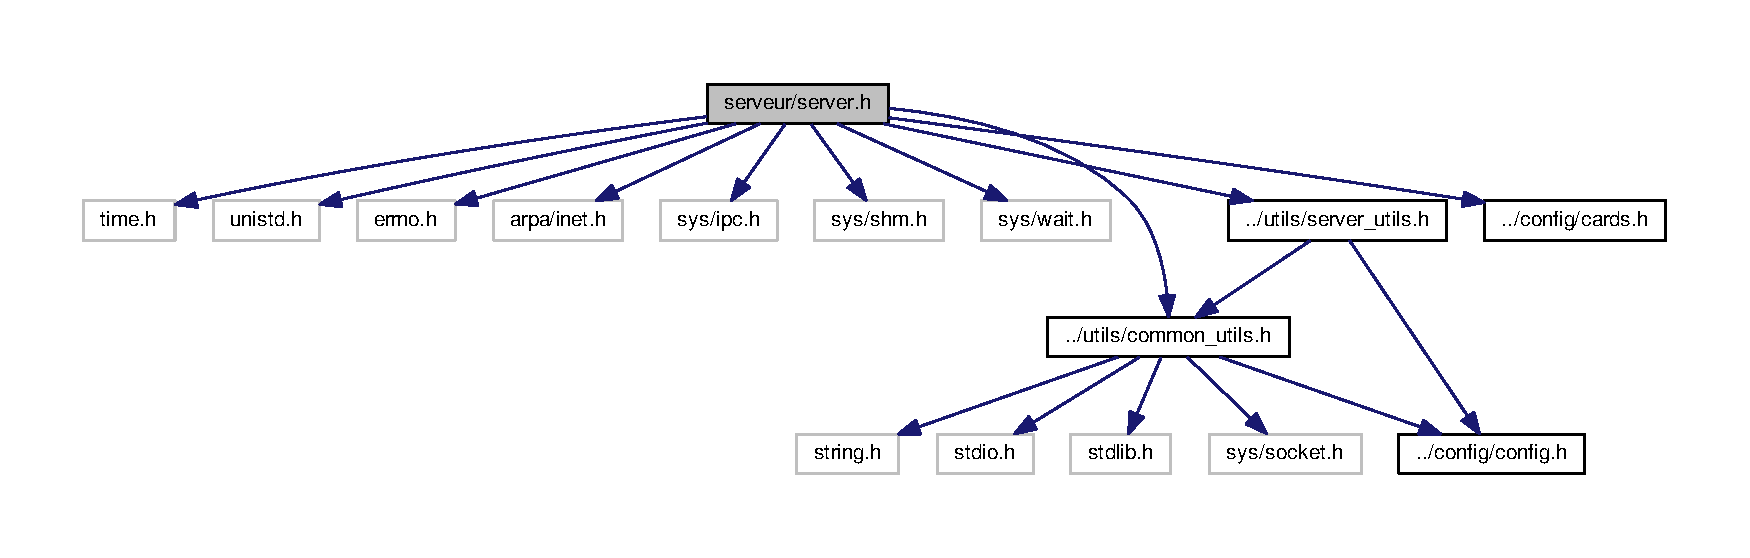
\includegraphics[width=350pt]{server_8h__incl}
\end{center}
\end{figure}
This graph shows which files directly or indirectly include this file\+:
\nopagebreak
\begin{figure}[H]
\begin{center}
\leavevmode
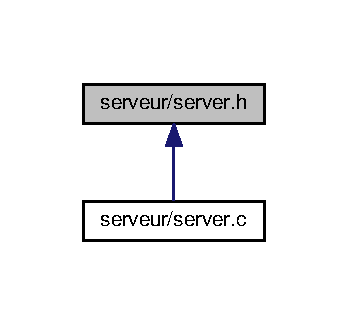
\includegraphics[width=167pt]{server_8h__dep__incl}
\end{center}
\end{figure}
\subsection*{Macros}
\begin{DoxyCompactItemize}
\item 
\#define \hyperlink{server_8h_ab1de365cca5246cc09e4bd07dbad5c29}{M\+I\+N\+\_\+\+P\+L\+A\+Y\+E\+RS}~2
\item 
\#define \hyperlink{server_8h_a614217d263be1fb1a5f76e2ff7be19a2}{P\+O\+RT}~\hyperlink{ports_8h_a1725876d3b41d0601d59768e442b7907}{P\+O\+R\+T\+\_\+\+D\+I\+M\+OV}
\item 
\#define \hyperlink{server_8h_a6b20d41d6252e9871430c242cb1a56e7}{B\+U\+F\+F\+E\+R\+\_\+\+S\+I\+ZE}~1024
\item 
\#define \hyperlink{server_8h_aeefbbafa97642defe3ee6c3080b7d66f}{B\+A\+C\+K\+L\+OG}~5
\item 
\#define \hyperlink{server_8h_a7c331dacb70e375dd02bfef709b71ea3}{C\+O\+U\+N\+T\+D\+O\+WN}~10
\end{DoxyCompactItemize}
\subsection*{Typedefs}
\begin{DoxyCompactItemize}
\item 
typedef void($\ast$ \hyperlink{server_8h_a6b8fa7d1c828463f6e6650a7dbc743e3}{fct\+\_\+ptr}) ()
\end{DoxyCompactItemize}
\subsection*{Functions}
\begin{DoxyCompactItemize}
\item 
void \hyperlink{server_8h_adbe4457a6e14fb0e0e5da917d6edd2d5}{init\+\_\+server} (int $\ast$, struct sockaddr\+\_\+in $\ast$)
\begin{DoxyCompactList}\small\item\em Fonction d\textquotesingle{}initialisation du serveur. \end{DoxyCompactList}\item 
void \hyperlink{server_8h_a9114ecbd0839e6cce5b379ebc11586bb}{alarm\+\_\+handler} (int)
\begin{DoxyCompactList}\small\item\em Fonction signal qui regarde s\textquotesingle{}il y a au moins deux joueurs. Sinon ça quitte le jeu. \end{DoxyCompactList}\item 
void \hyperlink{server_8h_abcbf6c09394bb6a1db56ecf5c888fb87}{interrupt\+\_\+handler} (int)
\begin{DoxyCompactList}\small\item\em Fonction de déconnexion d\textquotesingle{}un client suita à un controle C. \end{DoxyCompactList}\item 
void \hyperlink{server_8h_a30ce08aef9e75d64b27e69f6ce0756b6}{shutdown\+\_\+socket} (int)
\begin{DoxyCompactList}\small\item\em Fonction de fermeture de la socket. \end{DoxyCompactList}\item 
void \hyperlink{server_8h_a823119f7fbe44e03c0d173e74a595a0b}{shutdown\+\_\+server} ()
\begin{DoxyCompactList}\small\item\em Fonction de fermeture du serveur. \end{DoxyCompactList}\item 
void \hyperlink{server_8h_ad0bb1df570a4d34b036daf228388a0c1}{add\+\_\+client} (int, struct sockaddr\+\_\+in $\ast$)
\begin{DoxyCompactList}\small\item\em Fonction d\textquotesingle{}ajout d\textquotesingle{}un client au serveur. Si le jeu est en cours, on refuse la connexion S\textquotesingle{}il y a 4 personnes on ferme le lobby. \end{DoxyCompactList}\item 
void \hyperlink{server_8h_aa694be34287e456e5e22f60cedd022e5}{add\+\_\+player} (int)
\begin{DoxyCompactList}\small\item\em Fonction qio ajoute un joueur. \end{DoxyCompactList}\item 
void \hyperlink{server_8h_a5f5cfa1c29d50ae0940221fe0ad03651}{remove\+\_\+player} (\hyperlink{structplayer}{player} $\ast$, int, \hyperlink{config_8h_a1062901a7428fdd9c7f180f5e01ea056}{bool})
\begin{DoxyCompactList}\small\item\em Fonction qui retire un joueur. \end{DoxyCompactList}\item 
void \hyperlink{server_8h_a70b88da842b28ecee8ce334b84d1a9fa}{refuse\+\_\+connection} (int)
\begin{DoxyCompactList}\small\item\em Fonction de refus de connexion. Envoie d\textquotesingle{}un message avec le code R\+E\+F\+US défini dans \hyperlink{config_8h}{config.\+h}. \end{DoxyCompactList}\item 
\hyperlink{config_8h_a1062901a7428fdd9c7f180f5e01ea056}{bool} \hyperlink{server_8h_a0814d98ff87d4d6d4781f873bfdf4f39}{receive\+\_\+msg} (char $\ast$, int)
\begin{DoxyCompactList}\small\item\em Fonction de Récception de message du serveur. \end{DoxyCompactList}\item 
void \hyperlink{server_8h_ab9543a9dd0c09cdb40d921ea26308f80}{clear\+\_\+lobby} ()
\begin{DoxyCompactList}\small\item\em Fonction de nettoyage du lobby après qu\textquotesingle{}un joueur ait quitté le salon. \end{DoxyCompactList}\item 
void \hyperlink{server_8h_a586579926dbdc1e0c4b4fcecd2eacb7b}{add\+\_\+nickname} (int, char $\ast$$\ast$)
\begin{DoxyCompactList}\small\item\em Fonction qui ajoute le pseudo de 20 char max. \end{DoxyCompactList}\item 
void \hyperlink{server_8h_a671b58f5509a3a9fa692bacccfc32cc9}{start\+\_\+game} ()
\begin{DoxyCompactList}\small\item\em Fonction qui met le jeu en marche. Du coup, le jeu est en statut \+: \char`\"{}\+En cours\char`\"{}. \end{DoxyCompactList}\item 
void \hyperlink{server_8h_a528ee6cf05cb3b1af23306dc055e5eb3}{deal\+\_\+cards} ()
\begin{DoxyCompactList}\small\item\em Fonction de distribution des cartes. \end{DoxyCompactList}\item 
void \hyperlink{server_8h_ac81d67cd3689820d5a77d7a302a69e5c}{start\+\_\+round} ()
\begin{DoxyCompactList}\small\item\em Fonction de démarrage du round. \end{DoxyCompactList}\item 
void \hyperlink{server_8h_a0aba0f88abe71a413343d35ee5995683}{receive\+\_\+card} (int, char $\ast$$\ast$)
\begin{DoxyCompactList}\small\item\em Fonction de réception des cartes. \end{DoxyCompactList}\item 
void \hyperlink{server_8h_a26877a4a2039828bb05743dce8916132}{end\+\_\+round} (int, char $\ast$$\ast$)
\begin{DoxyCompactList}\small\item\em Fonction terminer un round. \end{DoxyCompactList}\item 
void \hyperlink{server_8h_afbb3dc95041fa32e01347ab80cc8c0fb}{update\+\_\+score} (int, char $\ast$$\ast$)
\begin{DoxyCompactList}\small\item\em Fonction de mise à jour du score. \end{DoxyCompactList}\item 
void \hyperlink{server_8h_a0801e69c9acfc06f40c84fc699d364d2}{create\+\_\+nicknames\+\_\+shared\+\_\+memory} (char $\ast$nickname)
\item 
void \hyperlink{server_8h_a4202fa5c5191c7e387d7570da6c8cd8c}{end\+\_\+game} ()
\begin{DoxyCompactList}\small\item\em Fonction de fin de jeu. \end{DoxyCompactList}\item 
int \hyperlink{server_8h_afdfc614e744d8d0a06fb97fd753b39c9}{find\+\_\+index} (\hyperlink{structplayer}{player} $\ast$, int)
\begin{DoxyCompactList}\small\item\em Fonction d\textquotesingle{}indexage des joueurs. \end{DoxyCompactList}\end{DoxyCompactItemize}


\subsection{Detailed Description}
Projet de M\+C\+S3 2016 2017. 

\begin{DoxyAuthor}{Author}
B\+E\+N\+C\+H\+I\+HA -\/ S\+A\+L\+E\+N\+G\+RO -\/ L\+E\+F\+O\+RT 
\end{DoxyAuthor}
\begin{DoxyVersion}{Version}
1 
\end{DoxyVersion}
\begin{DoxyDate}{Date}
D\+E\+C\+E\+M\+B\+RE -\/ J\+A\+N\+V\+I\+ER
\end{DoxyDate}
Fichier gérant les variables du serveur 

\subsection{Macro Definition Documentation}
\index{server.\+h@{server.\+h}!B\+A\+C\+K\+L\+OG@{B\+A\+C\+K\+L\+OG}}
\index{B\+A\+C\+K\+L\+OG@{B\+A\+C\+K\+L\+OG}!server.\+h@{server.\+h}}
\subsubsection[{\texorpdfstring{B\+A\+C\+K\+L\+OG}{BACKLOG}}]{\setlength{\rightskip}{0pt plus 5cm}\#define B\+A\+C\+K\+L\+OG~5}\hypertarget{server_8h_aeefbbafa97642defe3ee6c3080b7d66f}{}\label{server_8h_aeefbbafa97642defe3ee6c3080b7d66f}
\index{server.\+h@{server.\+h}!B\+U\+F\+F\+E\+R\+\_\+\+S\+I\+ZE@{B\+U\+F\+F\+E\+R\+\_\+\+S\+I\+ZE}}
\index{B\+U\+F\+F\+E\+R\+\_\+\+S\+I\+ZE@{B\+U\+F\+F\+E\+R\+\_\+\+S\+I\+ZE}!server.\+h@{server.\+h}}
\subsubsection[{\texorpdfstring{B\+U\+F\+F\+E\+R\+\_\+\+S\+I\+ZE}{BUFFER_SIZE}}]{\setlength{\rightskip}{0pt plus 5cm}\#define B\+U\+F\+F\+E\+R\+\_\+\+S\+I\+ZE~1024}\hypertarget{server_8h_a6b20d41d6252e9871430c242cb1a56e7}{}\label{server_8h_a6b20d41d6252e9871430c242cb1a56e7}
\index{server.\+h@{server.\+h}!C\+O\+U\+N\+T\+D\+O\+WN@{C\+O\+U\+N\+T\+D\+O\+WN}}
\index{C\+O\+U\+N\+T\+D\+O\+WN@{C\+O\+U\+N\+T\+D\+O\+WN}!server.\+h@{server.\+h}}
\subsubsection[{\texorpdfstring{C\+O\+U\+N\+T\+D\+O\+WN}{COUNTDOWN}}]{\setlength{\rightskip}{0pt plus 5cm}\#define C\+O\+U\+N\+T\+D\+O\+WN~10}\hypertarget{server_8h_a7c331dacb70e375dd02bfef709b71ea3}{}\label{server_8h_a7c331dacb70e375dd02bfef709b71ea3}
\index{server.\+h@{server.\+h}!M\+I\+N\+\_\+\+P\+L\+A\+Y\+E\+RS@{M\+I\+N\+\_\+\+P\+L\+A\+Y\+E\+RS}}
\index{M\+I\+N\+\_\+\+P\+L\+A\+Y\+E\+RS@{M\+I\+N\+\_\+\+P\+L\+A\+Y\+E\+RS}!server.\+h@{server.\+h}}
\subsubsection[{\texorpdfstring{M\+I\+N\+\_\+\+P\+L\+A\+Y\+E\+RS}{MIN_PLAYERS}}]{\setlength{\rightskip}{0pt plus 5cm}\#define M\+I\+N\+\_\+\+P\+L\+A\+Y\+E\+RS~2}\hypertarget{server_8h_ab1de365cca5246cc09e4bd07dbad5c29}{}\label{server_8h_ab1de365cca5246cc09e4bd07dbad5c29}
\index{server.\+h@{server.\+h}!P\+O\+RT@{P\+O\+RT}}
\index{P\+O\+RT@{P\+O\+RT}!server.\+h@{server.\+h}}
\subsubsection[{\texorpdfstring{P\+O\+RT}{PORT}}]{\setlength{\rightskip}{0pt plus 5cm}\#define P\+O\+RT~{\bf P\+O\+R\+T\+\_\+\+D\+I\+M\+OV}}\hypertarget{server_8h_a614217d263be1fb1a5f76e2ff7be19a2}{}\label{server_8h_a614217d263be1fb1a5f76e2ff7be19a2}


\subsection{Typedef Documentation}
\index{server.\+h@{server.\+h}!fct\+\_\+ptr@{fct\+\_\+ptr}}
\index{fct\+\_\+ptr@{fct\+\_\+ptr}!server.\+h@{server.\+h}}
\subsubsection[{\texorpdfstring{fct\+\_\+ptr}{fct_ptr}}]{\setlength{\rightskip}{0pt plus 5cm}typedef void($\ast$ fct\+\_\+ptr) ()}\hypertarget{server_8h_a6b8fa7d1c828463f6e6650a7dbc743e3}{}\label{server_8h_a6b8fa7d1c828463f6e6650a7dbc743e3}


\subsection{Function Documentation}
\index{server.\+h@{server.\+h}!add\+\_\+client@{add\+\_\+client}}
\index{add\+\_\+client@{add\+\_\+client}!server.\+h@{server.\+h}}
\subsubsection[{\texorpdfstring{add\+\_\+client(int, struct sockaddr\+\_\+in $\ast$)}{add_client(int, struct sockaddr_in *)}}]{\setlength{\rightskip}{0pt plus 5cm}void add\+\_\+client (
\begin{DoxyParamCaption}
\item[{int}]{server\+\_\+socket, }
\item[{struct sockaddr\+\_\+in $\ast$}]{cl\+\_\+addr}
\end{DoxyParamCaption}
)}\hypertarget{server_8h_ad0bb1df570a4d34b036daf228388a0c1}{}\label{server_8h_ad0bb1df570a4d34b036daf228388a0c1}


Fonction d\textquotesingle{}ajout d\textquotesingle{}un client au serveur. Si le jeu est en cours, on refuse la connexion S\textquotesingle{}il y a 4 personnes on ferme le lobby. 


\begin{DoxyParams}{Parameters}
{\em server\+\_\+socket} & \\
\hline
{\em $\ast$cl\+\_\+addr} & \\
\hline
\end{DoxyParams}
\begin{DoxyReturn}{Returns}
V\+O\+ID 
\end{DoxyReturn}
\index{server.\+h@{server.\+h}!add\+\_\+nickname@{add\+\_\+nickname}}
\index{add\+\_\+nickname@{add\+\_\+nickname}!server.\+h@{server.\+h}}
\subsubsection[{\texorpdfstring{add\+\_\+nickname(int, char $\ast$$\ast$)}{add_nickname(int, char **)}}]{\setlength{\rightskip}{0pt plus 5cm}void add\+\_\+nickname (
\begin{DoxyParamCaption}
\item[{int}]{socket, }
\item[{char $\ast$$\ast$}]{msg}
\end{DoxyParamCaption}
)}\hypertarget{server_8h_a586579926dbdc1e0c4b4fcecd2eacb7b}{}\label{server_8h_a586579926dbdc1e0c4b4fcecd2eacb7b}


Fonction qui ajoute le pseudo de 20 char max. 


\begin{DoxyParams}{Parameters}
{\em socket} & \\
\hline
{\em $\ast$$\ast$msg} & \\
\hline
\end{DoxyParams}
\begin{DoxyReturn}{Returns}
V\+O\+ID 
\end{DoxyReturn}
\index{server.\+h@{server.\+h}!add\+\_\+player@{add\+\_\+player}}
\index{add\+\_\+player@{add\+\_\+player}!server.\+h@{server.\+h}}
\subsubsection[{\texorpdfstring{add\+\_\+player(int)}{add_player(int)}}]{\setlength{\rightskip}{0pt plus 5cm}void add\+\_\+player (
\begin{DoxyParamCaption}
\item[{int}]{socket}
\end{DoxyParamCaption}
)}\hypertarget{server_8h_aa694be34287e456e5e22f60cedd022e5}{}\label{server_8h_aa694be34287e456e5e22f60cedd022e5}


Fonction qio ajoute un joueur. 


\begin{DoxyParams}{Parameters}
{\em socket} & \\
\hline
\end{DoxyParams}
\begin{DoxyReturn}{Returns}
V\+O\+ID 
\end{DoxyReturn}
\index{server.\+h@{server.\+h}!alarm\+\_\+handler@{alarm\+\_\+handler}}
\index{alarm\+\_\+handler@{alarm\+\_\+handler}!server.\+h@{server.\+h}}
\subsubsection[{\texorpdfstring{alarm\+\_\+handler(int)}{alarm_handler(int)}}]{\setlength{\rightskip}{0pt plus 5cm}void alarm\+\_\+handler (
\begin{DoxyParamCaption}
\item[{int}]{signum}
\end{DoxyParamCaption}
)}\hypertarget{server_8h_a9114ecbd0839e6cce5b379ebc11586bb}{}\label{server_8h_a9114ecbd0839e6cce5b379ebc11586bb}


Fonction signal qui regarde s\textquotesingle{}il y a au moins deux joueurs. Sinon ça quitte le jeu. 


\begin{DoxyParams}{Parameters}
{\em signum} & numéro du signal \\
\hline
\end{DoxyParams}
\begin{DoxyReturn}{Returns}
V\+O\+ID 
\end{DoxyReturn}
\index{server.\+h@{server.\+h}!clear\+\_\+lobby@{clear\+\_\+lobby}}
\index{clear\+\_\+lobby@{clear\+\_\+lobby}!server.\+h@{server.\+h}}
\subsubsection[{\texorpdfstring{clear\+\_\+lobby()}{clear_lobby()}}]{\setlength{\rightskip}{0pt plus 5cm}void clear\+\_\+lobby (
\begin{DoxyParamCaption}
{}
\end{DoxyParamCaption}
)}\hypertarget{server_8h_ab9543a9dd0c09cdb40d921ea26308f80}{}\label{server_8h_ab9543a9dd0c09cdb40d921ea26308f80}


Fonction de nettoyage du lobby après qu\textquotesingle{}un joueur ait quitté le salon. 


\begin{DoxyParams}{Parameters}
{\em V\+O\+ID} & \\
\hline
\end{DoxyParams}
\begin{DoxyReturn}{Returns}
V\+O\+ID 
\end{DoxyReturn}
\index{server.\+h@{server.\+h}!create\+\_\+nicknames\+\_\+shared\+\_\+memory@{create\+\_\+nicknames\+\_\+shared\+\_\+memory}}
\index{create\+\_\+nicknames\+\_\+shared\+\_\+memory@{create\+\_\+nicknames\+\_\+shared\+\_\+memory}!server.\+h@{server.\+h}}
\subsubsection[{\texorpdfstring{create\+\_\+nicknames\+\_\+shared\+\_\+memory(char $\ast$nickname)}{create_nicknames_shared_memory(char *nickname)}}]{\setlength{\rightskip}{0pt plus 5cm}void create\+\_\+nicknames\+\_\+shared\+\_\+memory (
\begin{DoxyParamCaption}
\item[{char $\ast$}]{nickname}
\end{DoxyParamCaption}
)}\hypertarget{server_8h_a0801e69c9acfc06f40c84fc699d364d2}{}\label{server_8h_a0801e69c9acfc06f40c84fc699d364d2}
\index{server.\+h@{server.\+h}!deal\+\_\+cards@{deal\+\_\+cards}}
\index{deal\+\_\+cards@{deal\+\_\+cards}!server.\+h@{server.\+h}}
\subsubsection[{\texorpdfstring{deal\+\_\+cards()}{deal_cards()}}]{\setlength{\rightskip}{0pt plus 5cm}void deal\+\_\+cards (
\begin{DoxyParamCaption}
{}
\end{DoxyParamCaption}
)}\hypertarget{server_8h_a528ee6cf05cb3b1af23306dc055e5eb3}{}\label{server_8h_a528ee6cf05cb3b1af23306dc055e5eb3}


Fonction de distribution des cartes. 


\begin{DoxyParams}{Parameters}
{\em void} & \\
\hline
\end{DoxyParams}
\begin{DoxyReturn}{Returns}
V\+O\+ID 
\end{DoxyReturn}
\index{server.\+h@{server.\+h}!end\+\_\+game@{end\+\_\+game}}
\index{end\+\_\+game@{end\+\_\+game}!server.\+h@{server.\+h}}
\subsubsection[{\texorpdfstring{end\+\_\+game()}{end_game()}}]{\setlength{\rightskip}{0pt plus 5cm}void end\+\_\+game (
\begin{DoxyParamCaption}
{}
\end{DoxyParamCaption}
)}\hypertarget{server_8h_a4202fa5c5191c7e387d7570da6c8cd8c}{}\label{server_8h_a4202fa5c5191c7e387d7570da6c8cd8c}


Fonction de fin de jeu. 


\begin{DoxyParams}{Parameters}
{\em information} & boolean qui va vérifier si on s\textquotesingle{}est déconnecté ou pas. \\
\hline
\end{DoxyParams}
\begin{DoxyReturn}{Returns}
V\+O\+ID 
\end{DoxyReturn}
\index{server.\+h@{server.\+h}!end\+\_\+round@{end\+\_\+round}}
\index{end\+\_\+round@{end\+\_\+round}!server.\+h@{server.\+h}}
\subsubsection[{\texorpdfstring{end\+\_\+round(int, char $\ast$$\ast$)}{end_round(int, char **)}}]{\setlength{\rightskip}{0pt plus 5cm}void end\+\_\+round (
\begin{DoxyParamCaption}
\item[{int}]{socket, }
\item[{char $\ast$$\ast$}]{msg}
\end{DoxyParamCaption}
)}\hypertarget{server_8h_a26877a4a2039828bb05743dce8916132}{}\label{server_8h_a26877a4a2039828bb05743dce8916132}


Fonction terminer un round. 


\begin{DoxyParams}{Parameters}
{\em socket} & \\
\hline
{\em $\ast$$\ast$msg} & \\
\hline
\end{DoxyParams}
\begin{DoxyReturn}{Returns}
V\+O\+ID 
\end{DoxyReturn}
\index{server.\+h@{server.\+h}!find\+\_\+index@{find\+\_\+index}}
\index{find\+\_\+index@{find\+\_\+index}!server.\+h@{server.\+h}}
\subsubsection[{\texorpdfstring{find\+\_\+index(player $\ast$, int)}{find_index(player *, int)}}]{\setlength{\rightskip}{0pt plus 5cm}int find\+\_\+index (
\begin{DoxyParamCaption}
\item[{{\bf player} $\ast$}]{joueurs, }
\item[{int}]{socket}
\end{DoxyParamCaption}
)}\hypertarget{server_8h_afdfc614e744d8d0a06fb97fd753b39c9}{}\label{server_8h_afdfc614e744d8d0a06fb97fd753b39c9}


Fonction d\textquotesingle{}indexage des joueurs. 


\begin{DoxyParams}{Parameters}
{\em joueurs} & structure de données défini dans \hyperlink{server__utils_8h}{server\+\_\+utils.\+h} \\
\hline
{\em socket} & \\
\hline
\end{DoxyParams}
\begin{DoxyReturn}{Returns}
int 
\end{DoxyReturn}
\index{server.\+h@{server.\+h}!init\+\_\+server@{init\+\_\+server}}
\index{init\+\_\+server@{init\+\_\+server}!server.\+h@{server.\+h}}
\subsubsection[{\texorpdfstring{init\+\_\+server(int $\ast$, struct sockaddr\+\_\+in $\ast$)}{init_server(int *, struct sockaddr_in *)}}]{\setlength{\rightskip}{0pt plus 5cm}void init\+\_\+server (
\begin{DoxyParamCaption}
\item[{int $\ast$}]{server\+\_\+socket, }
\item[{struct sockaddr\+\_\+in $\ast$}]{my\+\_\+addr}
\end{DoxyParamCaption}
)}\hypertarget{server_8h_adbe4457a6e14fb0e0e5da917d6edd2d5}{}\label{server_8h_adbe4457a6e14fb0e0e5da917d6edd2d5}


Fonction d\textquotesingle{}initialisation du serveur. 


\begin{DoxyParams}{Parameters}
{\em $\ast$server\+\_\+socket} & \\
\hline
{\em $\ast$my\+\_\+addr} & \\
\hline
\end{DoxyParams}
\begin{DoxyReturn}{Returns}
V\+O\+ID 
\end{DoxyReturn}
\index{server.\+h@{server.\+h}!interrupt\+\_\+handler@{interrupt\+\_\+handler}}
\index{interrupt\+\_\+handler@{interrupt\+\_\+handler}!server.\+h@{server.\+h}}
\subsubsection[{\texorpdfstring{interrupt\+\_\+handler(int)}{interrupt_handler(int)}}]{\setlength{\rightskip}{0pt plus 5cm}void interrupt\+\_\+handler (
\begin{DoxyParamCaption}
\item[{int}]{signum}
\end{DoxyParamCaption}
)}\hypertarget{server_8h_abcbf6c09394bb6a1db56ecf5c888fb87}{}\label{server_8h_abcbf6c09394bb6a1db56ecf5c888fb87}


Fonction de déconnexion d\textquotesingle{}un client suita à un controle C. 

Fonction de signal d\textquotesingle{}interruption.


\begin{DoxyParams}{Parameters}
{\em signum} & signal vérifiant le controle C \\
\hline
\end{DoxyParams}
\begin{DoxyReturn}{Returns}
V\+O\+ID.
\end{DoxyReturn}

\begin{DoxyParams}{Parameters}
{\em signum} & \\
\hline
\end{DoxyParams}
\begin{DoxyReturn}{Returns}
V\+O\+ID 
\end{DoxyReturn}
\index{server.\+h@{server.\+h}!receive\+\_\+card@{receive\+\_\+card}}
\index{receive\+\_\+card@{receive\+\_\+card}!server.\+h@{server.\+h}}
\subsubsection[{\texorpdfstring{receive\+\_\+card(int, char $\ast$$\ast$)}{receive_card(int, char **)}}]{\setlength{\rightskip}{0pt plus 5cm}void receive\+\_\+card (
\begin{DoxyParamCaption}
\item[{int}]{socket, }
\item[{char $\ast$$\ast$}]{msg}
\end{DoxyParamCaption}
)}\hypertarget{server_8h_a0aba0f88abe71a413343d35ee5995683}{}\label{server_8h_a0aba0f88abe71a413343d35ee5995683}


Fonction de réception des cartes. 


\begin{DoxyParams}{Parameters}
{\em socket} & \\
\hline
{\em $\ast$$\ast$msg} & \\
\hline
\end{DoxyParams}
\begin{DoxyReturn}{Returns}
V\+O\+ID 
\end{DoxyReturn}
\index{server.\+h@{server.\+h}!receive\+\_\+msg@{receive\+\_\+msg}}
\index{receive\+\_\+msg@{receive\+\_\+msg}!server.\+h@{server.\+h}}
\subsubsection[{\texorpdfstring{receive\+\_\+msg(char $\ast$, int)}{receive_msg(char *, int)}}]{\setlength{\rightskip}{0pt plus 5cm}{\bf bool} receive\+\_\+msg (
\begin{DoxyParamCaption}
\item[{char $\ast$}]{msg, }
\item[{int}]{fd}
\end{DoxyParamCaption}
)}\hypertarget{server_8h_a0814d98ff87d4d6d4781f873bfdf4f39}{}\label{server_8h_a0814d98ff87d4d6d4781f873bfdf4f39}


Fonction de Récception de message du serveur. 


\begin{DoxyParams}{Parameters}
{\em $\ast$msg} & \\
\hline
{\em fd} & \\
\hline
\end{DoxyParams}
\begin{DoxyReturn}{Returns}
bool 
\end{DoxyReturn}
\index{server.\+h@{server.\+h}!refuse\+\_\+connection@{refuse\+\_\+connection}}
\index{refuse\+\_\+connection@{refuse\+\_\+connection}!server.\+h@{server.\+h}}
\subsubsection[{\texorpdfstring{refuse\+\_\+connection(int)}{refuse_connection(int)}}]{\setlength{\rightskip}{0pt plus 5cm}void refuse\+\_\+connection (
\begin{DoxyParamCaption}
\item[{int}]{socket}
\end{DoxyParamCaption}
)}\hypertarget{server_8h_a70b88da842b28ecee8ce334b84d1a9fa}{}\label{server_8h_a70b88da842b28ecee8ce334b84d1a9fa}


Fonction de refus de connexion. Envoie d\textquotesingle{}un message avec le code R\+E\+F\+US défini dans \hyperlink{config_8h}{config.\+h}. 


\begin{DoxyParams}{Parameters}
{\em socket} & \\
\hline
\end{DoxyParams}
\begin{DoxyReturn}{Returns}
V\+O\+ID 
\end{DoxyReturn}
\index{server.\+h@{server.\+h}!remove\+\_\+player@{remove\+\_\+player}}
\index{remove\+\_\+player@{remove\+\_\+player}!server.\+h@{server.\+h}}
\subsubsection[{\texorpdfstring{remove\+\_\+player(player $\ast$, int, bool)}{remove_player(player *, int, bool)}}]{\setlength{\rightskip}{0pt plus 5cm}void remove\+\_\+player (
\begin{DoxyParamCaption}
\item[{{\bf player} $\ast$}]{joueurs, }
\item[{int}]{index, }
\item[{{\bf bool}}]{sockopen}
\end{DoxyParamCaption}
)}\hypertarget{server_8h_a5f5cfa1c29d50ae0940221fe0ad03651}{}\label{server_8h_a5f5cfa1c29d50ae0940221fe0ad03651}


Fonction qui retire un joueur. 


\begin{DoxyParams}{Parameters}
{\em joueur} & \\
\hline
{\em index} & \\
\hline
{\em sockopen} & \\
\hline
\end{DoxyParams}
\begin{DoxyReturn}{Returns}
V\+O\+ID 
\end{DoxyReturn}
\index{server.\+h@{server.\+h}!shutdown\+\_\+server@{shutdown\+\_\+server}}
\index{shutdown\+\_\+server@{shutdown\+\_\+server}!server.\+h@{server.\+h}}
\subsubsection[{\texorpdfstring{shutdown\+\_\+server()}{shutdown_server()}}]{\setlength{\rightskip}{0pt plus 5cm}void shutdown\+\_\+server (
\begin{DoxyParamCaption}
{}
\end{DoxyParamCaption}
)}\hypertarget{server_8h_a823119f7fbe44e03c0d173e74a595a0b}{}\label{server_8h_a823119f7fbe44e03c0d173e74a595a0b}


Fonction de fermeture du serveur. 


\begin{DoxyParams}{Parameters}
{\em void} & \\
\hline
\end{DoxyParams}
\begin{DoxyReturn}{Returns}
V\+O\+ID 
\end{DoxyReturn}
\index{server.\+h@{server.\+h}!shutdown\+\_\+socket@{shutdown\+\_\+socket}}
\index{shutdown\+\_\+socket@{shutdown\+\_\+socket}!server.\+h@{server.\+h}}
\subsubsection[{\texorpdfstring{shutdown\+\_\+socket(int)}{shutdown_socket(int)}}]{\setlength{\rightskip}{0pt plus 5cm}void shutdown\+\_\+socket (
\begin{DoxyParamCaption}
\item[{int}]{socket}
\end{DoxyParamCaption}
)}\hypertarget{server_8h_a30ce08aef9e75d64b27e69f6ce0756b6}{}\label{server_8h_a30ce08aef9e75d64b27e69f6ce0756b6}


Fonction de fermeture de la socket. 


\begin{DoxyParams}{Parameters}
{\em socket} & \\
\hline
\end{DoxyParams}
\begin{DoxyReturn}{Returns}
void 
\end{DoxyReturn}
\index{server.\+h@{server.\+h}!start\+\_\+game@{start\+\_\+game}}
\index{start\+\_\+game@{start\+\_\+game}!server.\+h@{server.\+h}}
\subsubsection[{\texorpdfstring{start\+\_\+game()}{start_game()}}]{\setlength{\rightskip}{0pt plus 5cm}void start\+\_\+game (
\begin{DoxyParamCaption}
{}
\end{DoxyParamCaption}
)}\hypertarget{server_8h_a671b58f5509a3a9fa692bacccfc32cc9}{}\label{server_8h_a671b58f5509a3a9fa692bacccfc32cc9}


Fonction qui met le jeu en marche. Du coup, le jeu est en statut \+: \char`\"{}\+En cours\char`\"{}. 


\begin{DoxyParams}{Parameters}
{\em V\+O\+ID} & \\
\hline
\end{DoxyParams}
\begin{DoxyReturn}{Returns}
V\+O\+ID 
\end{DoxyReturn}
\index{server.\+h@{server.\+h}!start\+\_\+round@{start\+\_\+round}}
\index{start\+\_\+round@{start\+\_\+round}!server.\+h@{server.\+h}}
\subsubsection[{\texorpdfstring{start\+\_\+round()}{start_round()}}]{\setlength{\rightskip}{0pt plus 5cm}void start\+\_\+round (
\begin{DoxyParamCaption}
{}
\end{DoxyParamCaption}
)}\hypertarget{server_8h_ac81d67cd3689820d5a77d7a302a69e5c}{}\label{server_8h_ac81d67cd3689820d5a77d7a302a69e5c}


Fonction de démarrage du round. 


\begin{DoxyParams}{Parameters}
{\em V\+O\+ID} & \\
\hline
\end{DoxyParams}
\begin{DoxyReturn}{Returns}
V\+O\+ID 
\end{DoxyReturn}
\index{server.\+h@{server.\+h}!update\+\_\+score@{update\+\_\+score}}
\index{update\+\_\+score@{update\+\_\+score}!server.\+h@{server.\+h}}
\subsubsection[{\texorpdfstring{update\+\_\+score(int, char $\ast$$\ast$)}{update_score(int, char **)}}]{\setlength{\rightskip}{0pt plus 5cm}void update\+\_\+score (
\begin{DoxyParamCaption}
\item[{int}]{socket, }
\item[{char $\ast$$\ast$}]{msg}
\end{DoxyParamCaption}
)}\hypertarget{server_8h_afbb3dc95041fa32e01347ab80cc8c0fb}{}\label{server_8h_afbb3dc95041fa32e01347ab80cc8c0fb}


Fonction de mise à jour du score. 


\begin{DoxyParams}{Parameters}
{\em socket} & \\
\hline
{\em $\ast$$\ast$msg} & \\
\hline
\end{DoxyParams}
\begin{DoxyReturn}{Returns}
V\+O\+ID 
\end{DoxyReturn}

\hypertarget{common__utils_8c}{}\section{utils/common\+\_\+utils.c File Reference}
\label{common__utils_8c}\index{utils/common\+\_\+utils.\+c@{utils/common\+\_\+utils.\+c}}


Projet de M\+C\+S3 2016 2017.  


{\ttfamily \#include \char`\"{}common\+\_\+utils.\+h\char`\"{}}\\*
Include dependency graph for common\+\_\+utils.\+c\+:
\nopagebreak
\begin{figure}[H]
\begin{center}
\leavevmode
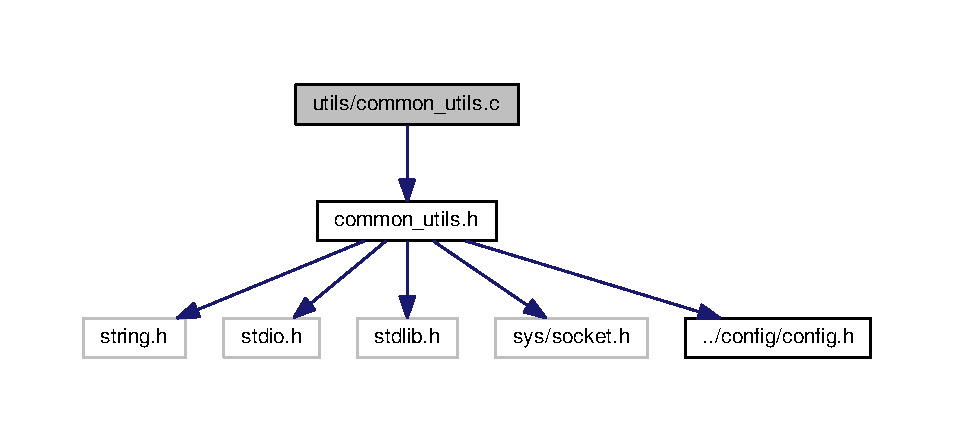
\includegraphics[width=350pt]{common__utils_8c__incl}
\end{center}
\end{figure}
\subsection*{Functions}
\begin{DoxyCompactItemize}
\item 
void \hyperlink{common__utils_8c_a1b072ac8427872e8a98ce851e63c83a6}{send\+\_\+prepared\+\_\+msg} (char $\ast$pmsg, int socket)
\begin{DoxyCompactList}\small\item\em Fonction d\textquotesingle{}envoie d\textquotesingle{}un message à une socket. \end{DoxyCompactList}\item 
void \hyperlink{common__utils_8c_ae4f3f9ada6d59ea5dec501237ddada3a}{send\+\_\+msg} (int msg\+\_\+code, const char $\ast$payload, int socket)
\begin{DoxyCompactList}\small\item\em Fonction d\textquotesingle{}envoie d\textquotesingle{}un message à une socket avec le code du message de type string. \end{DoxyCompactList}\item 
void \hyperlink{common__utils_8c_aaac454174096db6da8cdd9130187bac9}{send\+\_\+light\+\_\+msg} (int msg\+\_\+code, int socket)
\begin{DoxyCompactList}\small\item\em Fonction d\textquotesingle{}envoie d\textquotesingle{}un message à une socket sans le détaille. \end{DoxyCompactList}\item 
void \hyperlink{common__utils_8c_a53e6dc4a99bd00249494edba6e34bd35}{send\+\_\+int\+\_\+msg} (int msg\+\_\+code, int payload, int socket)
\begin{DoxyCompactList}\small\item\em Fonction d\textquotesingle{}envoie d\textquotesingle{}un message à une socket avec un code de type int. \end{DoxyCompactList}\item 
int \hyperlink{common__utils_8c_a1a4302eb8f903a67faf8903b0aeca91a}{extract\+\_\+msg\+\_\+code} (char $\ast$$\ast$msg)
\begin{DoxyCompactList}\small\item\em Fonction qui prend le code message. \end{DoxyCompactList}\item 
int \hyperlink{common__utils_8c_a162413542224a8c041274ce30269fa3b}{decode\+\_\+msg\+\_\+payload} (char $\ast$$\ast$raw\+\_\+payload, int $\ast$decoded\+\_\+payload, int max\+\_\+elements)
\begin{DoxyCompactList}\small\item\em Décoder le message passé en paramètre des fonctions. \end{DoxyCompactList}\end{DoxyCompactItemize}


\subsection{Detailed Description}
Projet de M\+C\+S3 2016 2017. 

\begin{DoxyAuthor}{Author}
B\+E\+N\+C\+H\+I\+HA -\/ S\+A\+L\+E\+N\+G\+RO -\/ L\+E\+F\+O\+RT 
\end{DoxyAuthor}
\begin{DoxyVersion}{Version}
1 
\end{DoxyVersion}
\begin{DoxyDate}{Date}
D\+E\+C\+E\+M\+B\+RE -\/ J\+A\+N\+V\+I\+ER
\end{DoxyDate}
Fichier gérant les fonctions utilisées par le client et le serveur M\+SG C\+O\+DE dans config 

\subsection{Function Documentation}
\index{common\+\_\+utils.\+c@{common\+\_\+utils.\+c}!decode\+\_\+msg\+\_\+payload@{decode\+\_\+msg\+\_\+payload}}
\index{decode\+\_\+msg\+\_\+payload@{decode\+\_\+msg\+\_\+payload}!common\+\_\+utils.\+c@{common\+\_\+utils.\+c}}
\subsubsection[{\texorpdfstring{decode\+\_\+msg\+\_\+payload(char $\ast$$\ast$raw\+\_\+payload, int $\ast$decoded\+\_\+payload, int max\+\_\+elements)}{decode_msg_payload(char **raw_payload, int *decoded_payload, int max_elements)}}]{\setlength{\rightskip}{0pt plus 5cm}int decode\+\_\+msg\+\_\+payload (
\begin{DoxyParamCaption}
\item[{char $\ast$$\ast$}]{raw\+\_\+payload, }
\item[{int $\ast$}]{decoded\+\_\+payload, }
\item[{int}]{max\+\_\+elements}
\end{DoxyParamCaption}
)}\hypertarget{common__utils_8c_a162413542224a8c041274ce30269fa3b}{}\label{common__utils_8c_a162413542224a8c041274ce30269fa3b}


Décoder le message passé en paramètre des fonctions. 


\begin{DoxyParams}{Parameters}
{\em $\ast$$\ast$raw\+\_\+payload} & \\
\hline
{\em $\ast$decode\+\_\+payload} & \\
\hline
{\em max\+\_\+elements} & \\
\hline
\end{DoxyParams}
\begin{DoxyReturn}{Returns}
int 
\end{DoxyReturn}
\index{common\+\_\+utils.\+c@{common\+\_\+utils.\+c}!extract\+\_\+msg\+\_\+code@{extract\+\_\+msg\+\_\+code}}
\index{extract\+\_\+msg\+\_\+code@{extract\+\_\+msg\+\_\+code}!common\+\_\+utils.\+c@{common\+\_\+utils.\+c}}
\subsubsection[{\texorpdfstring{extract\+\_\+msg\+\_\+code(char $\ast$$\ast$msg)}{extract_msg_code(char **msg)}}]{\setlength{\rightskip}{0pt plus 5cm}int extract\+\_\+msg\+\_\+code (
\begin{DoxyParamCaption}
\item[{char $\ast$$\ast$}]{msg}
\end{DoxyParamCaption}
)}\hypertarget{common__utils_8c_a1a4302eb8f903a67faf8903b0aeca91a}{}\label{common__utils_8c_a1a4302eb8f903a67faf8903b0aeca91a}


Fonction qui prend le code message. 


\begin{DoxyParams}{Parameters}
{\em $\ast$$\ast$msg} & \\
\hline
\end{DoxyParams}
\begin{DoxyReturn}{Returns}
int 
\end{DoxyReturn}
\index{common\+\_\+utils.\+c@{common\+\_\+utils.\+c}!send\+\_\+int\+\_\+msg@{send\+\_\+int\+\_\+msg}}
\index{send\+\_\+int\+\_\+msg@{send\+\_\+int\+\_\+msg}!common\+\_\+utils.\+c@{common\+\_\+utils.\+c}}
\subsubsection[{\texorpdfstring{send\+\_\+int\+\_\+msg(int msg\+\_\+code, int payload, int socket)}{send_int_msg(int msg_code, int payload, int socket)}}]{\setlength{\rightskip}{0pt plus 5cm}void send\+\_\+int\+\_\+msg (
\begin{DoxyParamCaption}
\item[{int}]{msg\+\_\+code, }
\item[{int}]{payload, }
\item[{int}]{socket}
\end{DoxyParamCaption}
)}\hypertarget{common__utils_8c_a53e6dc4a99bd00249494edba6e34bd35}{}\label{common__utils_8c_a53e6dc4a99bd00249494edba6e34bd35}


Fonction d\textquotesingle{}envoie d\textquotesingle{}un message à une socket avec un code de type int. 


\begin{DoxyParams}{Parameters}
{\em msg\+\_\+code} & \\
\hline
{\em payload} & \\
\hline
{\em socket} & \\
\hline
\end{DoxyParams}
\begin{DoxyReturn}{Returns}
V\+O\+ID 
\end{DoxyReturn}
\index{common\+\_\+utils.\+c@{common\+\_\+utils.\+c}!send\+\_\+light\+\_\+msg@{send\+\_\+light\+\_\+msg}}
\index{send\+\_\+light\+\_\+msg@{send\+\_\+light\+\_\+msg}!common\+\_\+utils.\+c@{common\+\_\+utils.\+c}}
\subsubsection[{\texorpdfstring{send\+\_\+light\+\_\+msg(int msg\+\_\+code, int socket)}{send_light_msg(int msg_code, int socket)}}]{\setlength{\rightskip}{0pt plus 5cm}void send\+\_\+light\+\_\+msg (
\begin{DoxyParamCaption}
\item[{int}]{msg\+\_\+code, }
\item[{int}]{socket}
\end{DoxyParamCaption}
)}\hypertarget{common__utils_8c_aaac454174096db6da8cdd9130187bac9}{}\label{common__utils_8c_aaac454174096db6da8cdd9130187bac9}


Fonction d\textquotesingle{}envoie d\textquotesingle{}un message à une socket sans le détaille. 


\begin{DoxyParams}{Parameters}
{\em msg\+\_\+code} & \\
\hline
{\em socket} & \\
\hline
\end{DoxyParams}
\begin{DoxyReturn}{Returns}
V\+O\+ID 
\end{DoxyReturn}
\index{common\+\_\+utils.\+c@{common\+\_\+utils.\+c}!send\+\_\+msg@{send\+\_\+msg}}
\index{send\+\_\+msg@{send\+\_\+msg}!common\+\_\+utils.\+c@{common\+\_\+utils.\+c}}
\subsubsection[{\texorpdfstring{send\+\_\+msg(int msg\+\_\+code, const char $\ast$payload, int socket)}{send_msg(int msg_code, const char *payload, int socket)}}]{\setlength{\rightskip}{0pt plus 5cm}void send\+\_\+msg (
\begin{DoxyParamCaption}
\item[{int}]{msg\+\_\+code, }
\item[{const char $\ast$}]{payload, }
\item[{int}]{socket}
\end{DoxyParamCaption}
)}\hypertarget{common__utils_8c_ae4f3f9ada6d59ea5dec501237ddada3a}{}\label{common__utils_8c_ae4f3f9ada6d59ea5dec501237ddada3a}


Fonction d\textquotesingle{}envoie d\textquotesingle{}un message à une socket avec le code du message de type string. 


\begin{DoxyParams}{Parameters}
{\em msg\+\_\+code} & \\
\hline
{\em $\ast$payload} & \\
\hline
{\em socket} & \\
\hline
\end{DoxyParams}
\begin{DoxyReturn}{Returns}
V\+O\+ID 
\end{DoxyReturn}
\index{common\+\_\+utils.\+c@{common\+\_\+utils.\+c}!send\+\_\+prepared\+\_\+msg@{send\+\_\+prepared\+\_\+msg}}
\index{send\+\_\+prepared\+\_\+msg@{send\+\_\+prepared\+\_\+msg}!common\+\_\+utils.\+c@{common\+\_\+utils.\+c}}
\subsubsection[{\texorpdfstring{send\+\_\+prepared\+\_\+msg(char $\ast$pmsg, int socket)}{send_prepared_msg(char *pmsg, int socket)}}]{\setlength{\rightskip}{0pt plus 5cm}void send\+\_\+prepared\+\_\+msg (
\begin{DoxyParamCaption}
\item[{char $\ast$}]{msg, }
\item[{int}]{socket}
\end{DoxyParamCaption}
)}\hypertarget{common__utils_8c_a1b072ac8427872e8a98ce851e63c83a6}{}\label{common__utils_8c_a1b072ac8427872e8a98ce851e63c83a6}


Fonction d\textquotesingle{}envoie d\textquotesingle{}un message à une socket. 


\begin{DoxyParams}{Parameters}
{\em $\ast$msg} & \\
\hline
{\em socket} & \\
\hline
\end{DoxyParams}
\begin{DoxyReturn}{Returns}
V\+O\+ID 
\end{DoxyReturn}

\hypertarget{common__utils_8h}{}\section{utils/common\+\_\+utils.h File Reference}
\label{common__utils_8h}\index{utils/common\+\_\+utils.\+h@{utils/common\+\_\+utils.\+h}}


Projet de M\+C\+S3 2016 2017.  


{\ttfamily \#include $<$string.\+h$>$}\\*
{\ttfamily \#include $<$stdio.\+h$>$}\\*
{\ttfamily \#include $<$stdlib.\+h$>$}\\*
{\ttfamily \#include $<$sys/socket.\+h$>$}\\*
{\ttfamily \#include \char`\"{}../config/config.\+h\char`\"{}}\\*
Include dependency graph for common\+\_\+utils.\+h\+:
\nopagebreak
\begin{figure}[H]
\begin{center}
\leavevmode
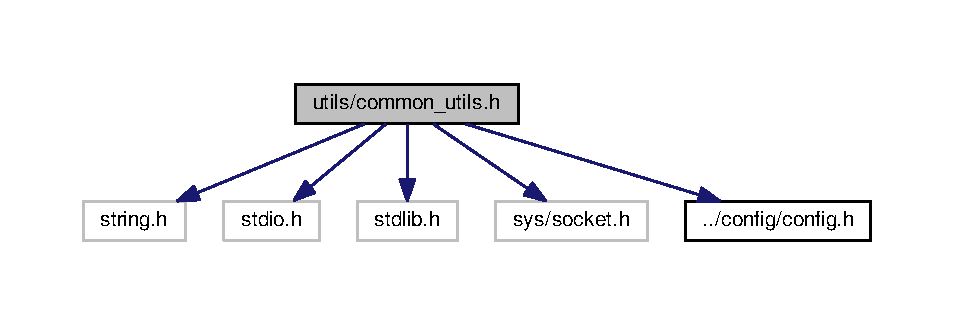
\includegraphics[width=350pt]{common__utils_8h__incl}
\end{center}
\end{figure}
This graph shows which files directly or indirectly include this file\+:
\nopagebreak
\begin{figure}[H]
\begin{center}
\leavevmode
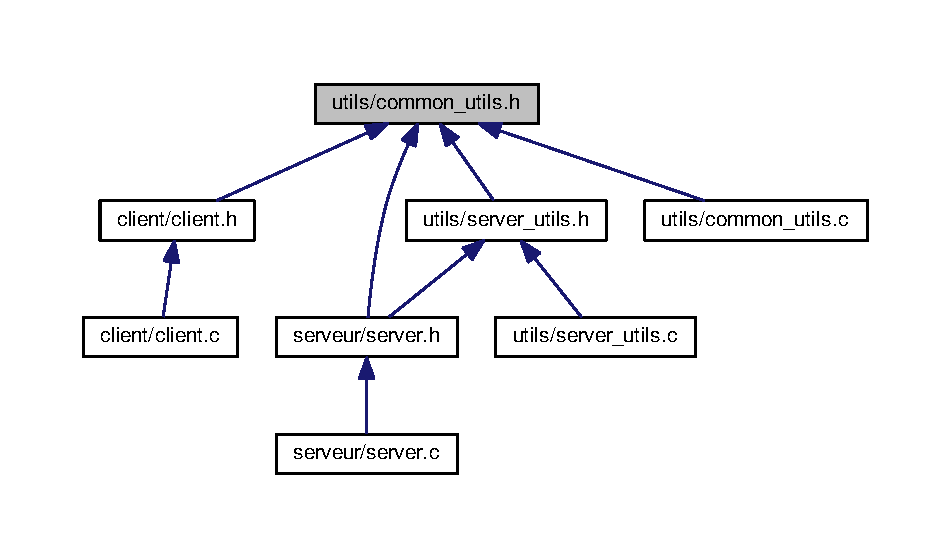
\includegraphics[width=350pt]{common__utils_8h__dep__incl}
\end{center}
\end{figure}
\subsection*{Macros}
\begin{DoxyCompactItemize}
\item 
\#define \hyperlink{common__utils_8h_aeca90e1c1c62b70670514ffc18c9dfd4}{M\+E\+S\+S\+A\+G\+E\+\_\+\+S\+I\+ZE}~82
\end{DoxyCompactItemize}
\subsection*{Functions}
\begin{DoxyCompactItemize}
\item 
void \hyperlink{common__utils_8h_a4ade57c5f924fe552632b38b1a20ab0a}{send\+\_\+prepared\+\_\+msg} (char $\ast$msg, int socket)
\begin{DoxyCompactList}\small\item\em Fonction d\textquotesingle{}envoie d\textquotesingle{}un message à une socket. \end{DoxyCompactList}\item 
void \hyperlink{common__utils_8h_ae4f3f9ada6d59ea5dec501237ddada3a}{send\+\_\+msg} (int msg\+\_\+code, const char $\ast$payload, int socket)
\begin{DoxyCompactList}\small\item\em Fonction d\textquotesingle{}envoie d\textquotesingle{}un message à une socket avec le code du message de type string. \end{DoxyCompactList}\item 
void \hyperlink{common__utils_8h_aaac454174096db6da8cdd9130187bac9}{send\+\_\+light\+\_\+msg} (int msg\+\_\+code, int socket)
\begin{DoxyCompactList}\small\item\em Fonction d\textquotesingle{}envoie d\textquotesingle{}un message à une socket sans le détaille. \end{DoxyCompactList}\item 
void \hyperlink{common__utils_8h_a53e6dc4a99bd00249494edba6e34bd35}{send\+\_\+int\+\_\+msg} (int msg\+\_\+code, int payload, int socket)
\begin{DoxyCompactList}\small\item\em Fonction d\textquotesingle{}envoie d\textquotesingle{}un message à une socket avec un code de type int. \end{DoxyCompactList}\item 
int \hyperlink{common__utils_8h_a1a4302eb8f903a67faf8903b0aeca91a}{extract\+\_\+msg\+\_\+code} (char $\ast$$\ast$msg)
\begin{DoxyCompactList}\small\item\em Fonction qui prend le code message. \end{DoxyCompactList}\item 
int \hyperlink{common__utils_8h_a162413542224a8c041274ce30269fa3b}{decode\+\_\+msg\+\_\+payload} (char $\ast$$\ast$raw\+\_\+payload, int $\ast$decoded\+\_\+payload, int max\+\_\+elements)
\begin{DoxyCompactList}\small\item\em Décoder le message passé en paramètre des fonctions. \end{DoxyCompactList}\end{DoxyCompactItemize}


\subsection{Detailed Description}
Projet de M\+C\+S3 2016 2017. 

\begin{DoxyAuthor}{Author}
B\+E\+N\+C\+H\+I\+HA -\/ S\+A\+L\+E\+N\+G\+RO -\/ L\+E\+F\+O\+RT 
\end{DoxyAuthor}
\begin{DoxyVersion}{Version}
1 
\end{DoxyVersion}
\begin{DoxyDate}{Date}
D\+E\+C\+E\+M\+B\+RE -\/ J\+A\+N\+V\+I\+ER
\end{DoxyDate}
Fichier gérant les fonctions utilisées par le client et le serveur 

\subsection{Macro Definition Documentation}
\index{common\+\_\+utils.\+h@{common\+\_\+utils.\+h}!M\+E\+S\+S\+A\+G\+E\+\_\+\+S\+I\+ZE@{M\+E\+S\+S\+A\+G\+E\+\_\+\+S\+I\+ZE}}
\index{M\+E\+S\+S\+A\+G\+E\+\_\+\+S\+I\+ZE@{M\+E\+S\+S\+A\+G\+E\+\_\+\+S\+I\+ZE}!common\+\_\+utils.\+h@{common\+\_\+utils.\+h}}
\subsubsection[{\texorpdfstring{M\+E\+S\+S\+A\+G\+E\+\_\+\+S\+I\+ZE}{MESSAGE_SIZE}}]{\setlength{\rightskip}{0pt plus 5cm}\#define M\+E\+S\+S\+A\+G\+E\+\_\+\+S\+I\+ZE~82}\hypertarget{common__utils_8h_aeca90e1c1c62b70670514ffc18c9dfd4}{}\label{common__utils_8h_aeca90e1c1c62b70670514ffc18c9dfd4}


\subsection{Function Documentation}
\index{common\+\_\+utils.\+h@{common\+\_\+utils.\+h}!decode\+\_\+msg\+\_\+payload@{decode\+\_\+msg\+\_\+payload}}
\index{decode\+\_\+msg\+\_\+payload@{decode\+\_\+msg\+\_\+payload}!common\+\_\+utils.\+h@{common\+\_\+utils.\+h}}
\subsubsection[{\texorpdfstring{decode\+\_\+msg\+\_\+payload(char $\ast$$\ast$raw\+\_\+payload, int $\ast$decoded\+\_\+payload, int max\+\_\+elements)}{decode_msg_payload(char **raw_payload, int *decoded_payload, int max_elements)}}]{\setlength{\rightskip}{0pt plus 5cm}int decode\+\_\+msg\+\_\+payload (
\begin{DoxyParamCaption}
\item[{char $\ast$$\ast$}]{raw\+\_\+payload, }
\item[{int $\ast$}]{decoded\+\_\+payload, }
\item[{int}]{max\+\_\+elements}
\end{DoxyParamCaption}
)}\hypertarget{common__utils_8h_a162413542224a8c041274ce30269fa3b}{}\label{common__utils_8h_a162413542224a8c041274ce30269fa3b}


Décoder le message passé en paramètre des fonctions. 


\begin{DoxyParams}{Parameters}
{\em $\ast$$\ast$raw\+\_\+payload} & \\
\hline
{\em $\ast$decode\+\_\+payload} & \\
\hline
{\em max\+\_\+elements} & \\
\hline
\end{DoxyParams}
\begin{DoxyReturn}{Returns}
int 
\end{DoxyReturn}
\index{common\+\_\+utils.\+h@{common\+\_\+utils.\+h}!extract\+\_\+msg\+\_\+code@{extract\+\_\+msg\+\_\+code}}
\index{extract\+\_\+msg\+\_\+code@{extract\+\_\+msg\+\_\+code}!common\+\_\+utils.\+h@{common\+\_\+utils.\+h}}
\subsubsection[{\texorpdfstring{extract\+\_\+msg\+\_\+code(char $\ast$$\ast$msg)}{extract_msg_code(char **msg)}}]{\setlength{\rightskip}{0pt plus 5cm}int extract\+\_\+msg\+\_\+code (
\begin{DoxyParamCaption}
\item[{char $\ast$$\ast$}]{msg}
\end{DoxyParamCaption}
)}\hypertarget{common__utils_8h_a1a4302eb8f903a67faf8903b0aeca91a}{}\label{common__utils_8h_a1a4302eb8f903a67faf8903b0aeca91a}


Fonction qui prend le code message. 


\begin{DoxyParams}{Parameters}
{\em $\ast$$\ast$msg} & \\
\hline
\end{DoxyParams}
\begin{DoxyReturn}{Returns}
int 
\end{DoxyReturn}
\index{common\+\_\+utils.\+h@{common\+\_\+utils.\+h}!send\+\_\+int\+\_\+msg@{send\+\_\+int\+\_\+msg}}
\index{send\+\_\+int\+\_\+msg@{send\+\_\+int\+\_\+msg}!common\+\_\+utils.\+h@{common\+\_\+utils.\+h}}
\subsubsection[{\texorpdfstring{send\+\_\+int\+\_\+msg(int msg\+\_\+code, int payload, int socket)}{send_int_msg(int msg_code, int payload, int socket)}}]{\setlength{\rightskip}{0pt plus 5cm}void send\+\_\+int\+\_\+msg (
\begin{DoxyParamCaption}
\item[{int}]{msg\+\_\+code, }
\item[{int}]{payload, }
\item[{int}]{socket}
\end{DoxyParamCaption}
)}\hypertarget{common__utils_8h_a53e6dc4a99bd00249494edba6e34bd35}{}\label{common__utils_8h_a53e6dc4a99bd00249494edba6e34bd35}


Fonction d\textquotesingle{}envoie d\textquotesingle{}un message à une socket avec un code de type int. 


\begin{DoxyParams}{Parameters}
{\em msg\+\_\+code} & \\
\hline
{\em payload} & \\
\hline
{\em socket} & \\
\hline
\end{DoxyParams}
\begin{DoxyReturn}{Returns}
V\+O\+ID 
\end{DoxyReturn}
\index{common\+\_\+utils.\+h@{common\+\_\+utils.\+h}!send\+\_\+light\+\_\+msg@{send\+\_\+light\+\_\+msg}}
\index{send\+\_\+light\+\_\+msg@{send\+\_\+light\+\_\+msg}!common\+\_\+utils.\+h@{common\+\_\+utils.\+h}}
\subsubsection[{\texorpdfstring{send\+\_\+light\+\_\+msg(int msg\+\_\+code, int socket)}{send_light_msg(int msg_code, int socket)}}]{\setlength{\rightskip}{0pt plus 5cm}void send\+\_\+light\+\_\+msg (
\begin{DoxyParamCaption}
\item[{int}]{msg\+\_\+code, }
\item[{int}]{socket}
\end{DoxyParamCaption}
)}\hypertarget{common__utils_8h_aaac454174096db6da8cdd9130187bac9}{}\label{common__utils_8h_aaac454174096db6da8cdd9130187bac9}


Fonction d\textquotesingle{}envoie d\textquotesingle{}un message à une socket sans le détaille. 


\begin{DoxyParams}{Parameters}
{\em msg\+\_\+code} & \\
\hline
{\em socket} & \\
\hline
\end{DoxyParams}
\begin{DoxyReturn}{Returns}
V\+O\+ID 
\end{DoxyReturn}
\index{common\+\_\+utils.\+h@{common\+\_\+utils.\+h}!send\+\_\+msg@{send\+\_\+msg}}
\index{send\+\_\+msg@{send\+\_\+msg}!common\+\_\+utils.\+h@{common\+\_\+utils.\+h}}
\subsubsection[{\texorpdfstring{send\+\_\+msg(int msg\+\_\+code, const char $\ast$payload, int socket)}{send_msg(int msg_code, const char *payload, int socket)}}]{\setlength{\rightskip}{0pt plus 5cm}void send\+\_\+msg (
\begin{DoxyParamCaption}
\item[{int}]{msg\+\_\+code, }
\item[{const char $\ast$}]{payload, }
\item[{int}]{socket}
\end{DoxyParamCaption}
)}\hypertarget{common__utils_8h_ae4f3f9ada6d59ea5dec501237ddada3a}{}\label{common__utils_8h_ae4f3f9ada6d59ea5dec501237ddada3a}


Fonction d\textquotesingle{}envoie d\textquotesingle{}un message à une socket avec le code du message de type string. 


\begin{DoxyParams}{Parameters}
{\em msg\+\_\+code} & \\
\hline
{\em $\ast$payload} & \\
\hline
{\em socket} & \\
\hline
\end{DoxyParams}
\begin{DoxyReturn}{Returns}
V\+O\+ID 
\end{DoxyReturn}
\index{common\+\_\+utils.\+h@{common\+\_\+utils.\+h}!send\+\_\+prepared\+\_\+msg@{send\+\_\+prepared\+\_\+msg}}
\index{send\+\_\+prepared\+\_\+msg@{send\+\_\+prepared\+\_\+msg}!common\+\_\+utils.\+h@{common\+\_\+utils.\+h}}
\subsubsection[{\texorpdfstring{send\+\_\+prepared\+\_\+msg(char $\ast$msg, int socket)}{send_prepared_msg(char *msg, int socket)}}]{\setlength{\rightskip}{0pt plus 5cm}void send\+\_\+prepared\+\_\+msg (
\begin{DoxyParamCaption}
\item[{char $\ast$}]{pmsg, }
\item[{int}]{socket}
\end{DoxyParamCaption}
)}\hypertarget{common__utils_8h_a4ade57c5f924fe552632b38b1a20ab0a}{}\label{common__utils_8h_a4ade57c5f924fe552632b38b1a20ab0a}


Fonction d\textquotesingle{}envoie d\textquotesingle{}un message à une socket. 


\begin{DoxyParams}{Parameters}
{\em $\ast$msg} & \\
\hline
{\em socket} & \\
\hline
\end{DoxyParams}
\begin{DoxyReturn}{Returns}
V\+O\+ID 
\end{DoxyReturn}

\hypertarget{server__utils_8c}{}\section{utils/server\+\_\+utils.c File Reference}
\label{server__utils_8c}\index{utils/server\+\_\+utils.\+c@{utils/server\+\_\+utils.\+c}}


Projet de M\+C\+S3 2016 2017.  


{\ttfamily \#include \char`\"{}server\+\_\+utils.\+h\char`\"{}}\\*
Include dependency graph for server\+\_\+utils.\+c\+:
\nopagebreak
\begin{figure}[H]
\begin{center}
\leavevmode
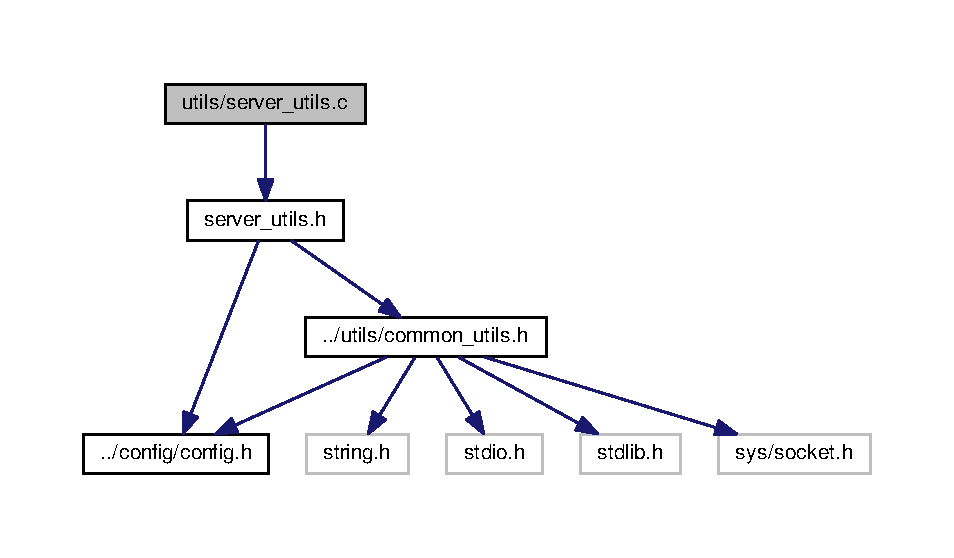
\includegraphics[width=350pt]{server__utils_8c__incl}
\end{center}
\end{figure}
\subsection*{Functions}
\begin{DoxyCompactItemize}
\item 
void \hyperlink{server__utils_8c_a763eeda4c9bfa1baf4151b50d541c1e9}{broadcast} (int msg\+\_\+code, char $\ast$payload, \hyperlink{structplayer}{player} $\ast$recipients, int rcp\+\_\+count)
\begin{DoxyCompactList}\small\item\em Diffusion du message envoyé au serveur. \end{DoxyCompactList}\item 
void \hyperlink{server__utils_8c_a4ad5d5d2094d030edbdd5085d87aaa6a}{broadcast\+\_\+light} (int msg\+\_\+code, \hyperlink{structplayer}{player} $\ast$recipients, int rcp\+\_\+count)
\begin{DoxyCompactList}\small\item\em Diffusion du message envoyé au serveur sans le corps du message. \end{DoxyCompactList}\item 
void \hyperlink{server__utils_8c_a3d194b02ce3591f5f20ac0db06e0b06d}{extract\+\_\+player\+\_\+nickname} (char $\ast$$\ast$msg, char $\ast$nickname)
\begin{DoxyCompactList}\small\item\em Fonction qui extrait le nom du joueur envoyé au serveur. \end{DoxyCompactList}\item 
int \hyperlink{server__utils_8c_ab7cc3806641017bc96af6fd10cabba98}{rand\+\_\+range} (int upper\+\_\+limit)
\begin{DoxyCompactList}\small\item\em Fonction qui génère un nombre aléatoire dans le max de upperlimite. \end{DoxyCompactList}\item 
\hyperlink{config_8h_a1062901a7428fdd9c7f180f5e01ea056}{bool} \hyperlink{server__utils_8c_a5dc1c39eb1f151b25bd0a5067aa8b594}{array\+\_\+contains} (int $\ast$haystack, int needle, int length)
\end{DoxyCompactItemize}


\subsection{Detailed Description}
Projet de M\+C\+S3 2016 2017. 

\begin{DoxyAuthor}{Author}
B\+E\+N\+C\+H\+I\+HA -\/ S\+A\+L\+E\+N\+G\+RO -\/ L\+E\+F\+O\+RT 
\end{DoxyAuthor}
\begin{DoxyVersion}{Version}
1 
\end{DoxyVersion}
\begin{DoxyDate}{Date}
D\+E\+C\+E\+M\+B\+RE -\/ J\+A\+N\+V\+I\+ER
\end{DoxyDate}
Fichier gérant les fonctions utilisées par le serveur 

\subsection{Function Documentation}
\index{server\+\_\+utils.\+c@{server\+\_\+utils.\+c}!array\+\_\+contains@{array\+\_\+contains}}
\index{array\+\_\+contains@{array\+\_\+contains}!server\+\_\+utils.\+c@{server\+\_\+utils.\+c}}
\subsubsection[{\texorpdfstring{array\+\_\+contains(int $\ast$haystack, int needle, int length)}{array_contains(int *haystack, int needle, int length)}}]{\setlength{\rightskip}{0pt plus 5cm}{\bf bool} array\+\_\+contains (
\begin{DoxyParamCaption}
\item[{int $\ast$}]{haystack, }
\item[{int}]{needle, }
\item[{int}]{length}
\end{DoxyParamCaption}
)}\hypertarget{server__utils_8c_a5dc1c39eb1f151b25bd0a5067aa8b594}{}\label{server__utils_8c_a5dc1c39eb1f151b25bd0a5067aa8b594}
\index{server\+\_\+utils.\+c@{server\+\_\+utils.\+c}!broadcast@{broadcast}}
\index{broadcast@{broadcast}!server\+\_\+utils.\+c@{server\+\_\+utils.\+c}}
\subsubsection[{\texorpdfstring{broadcast(int msg\+\_\+code, char $\ast$payload, player $\ast$recipients, int rcp\+\_\+count)}{broadcast(int msg_code, char *payload, player *recipients, int rcp_count)}}]{\setlength{\rightskip}{0pt plus 5cm}broadcast (
\begin{DoxyParamCaption}
\item[{int}]{msg\+\_\+code, }
\item[{char $\ast$}]{payload, }
\item[{{\bf player} $\ast$}]{recipients, }
\item[{int}]{rcp\+\_\+count}
\end{DoxyParamCaption}
)}\hypertarget{server__utils_8c_a763eeda4c9bfa1baf4151b50d541c1e9}{}\label{server__utils_8c_a763eeda4c9bfa1baf4151b50d541c1e9}


Diffusion du message envoyé au serveur. 


\begin{DoxyParams}{Parameters}
{\em msg\+\_\+code} & \\
\hline
{\em $\ast$payload} & \\
\hline
{\em $\ast$recipients} & \\
\hline
{\em rcp\+\_\+count} & \\
\hline
\end{DoxyParams}
\begin{DoxyReturn}{Returns}
V\+O\+ID 
\end{DoxyReturn}
\index{server\+\_\+utils.\+c@{server\+\_\+utils.\+c}!broadcast\+\_\+light@{broadcast\+\_\+light}}
\index{broadcast\+\_\+light@{broadcast\+\_\+light}!server\+\_\+utils.\+c@{server\+\_\+utils.\+c}}
\subsubsection[{\texorpdfstring{broadcast\+\_\+light(int msg\+\_\+code, player $\ast$recipients, int rcp\+\_\+count)}{broadcast_light(int msg_code, player *recipients, int rcp_count)}}]{\setlength{\rightskip}{0pt plus 5cm}broadcast\+\_\+light (
\begin{DoxyParamCaption}
\item[{int}]{msg\+\_\+code, }
\item[{{\bf player} $\ast$}]{recipients, }
\item[{int}]{rcp\+\_\+count}
\end{DoxyParamCaption}
)}\hypertarget{server__utils_8c_a4ad5d5d2094d030edbdd5085d87aaa6a}{}\label{server__utils_8c_a4ad5d5d2094d030edbdd5085d87aaa6a}


Diffusion du message envoyé au serveur sans le corps du message. 


\begin{DoxyParams}{Parameters}
{\em msg\+\_\+code} & \\
\hline
{\em $\ast$payload} & \\
\hline
{\em $\ast$recipients} & \\
\hline
{\em rcp\+\_\+count} & \\
\hline
\end{DoxyParams}
\begin{DoxyReturn}{Returns}
V\+O\+ID 
\end{DoxyReturn}
\index{server\+\_\+utils.\+c@{server\+\_\+utils.\+c}!extract\+\_\+player\+\_\+nickname@{extract\+\_\+player\+\_\+nickname}}
\index{extract\+\_\+player\+\_\+nickname@{extract\+\_\+player\+\_\+nickname}!server\+\_\+utils.\+c@{server\+\_\+utils.\+c}}
\subsubsection[{\texorpdfstring{extract\+\_\+player\+\_\+nickname(char $\ast$$\ast$msg, char $\ast$nickname)}{extract_player_nickname(char **msg, char *nickname)}}]{\setlength{\rightskip}{0pt plus 5cm}extract\+\_\+player\+\_\+nickname (
\begin{DoxyParamCaption}
\item[{char $\ast$$\ast$}]{msg, }
\item[{char $\ast$}]{nickname}
\end{DoxyParamCaption}
)}\hypertarget{server__utils_8c_a3d194b02ce3591f5f20ac0db06e0b06d}{}\label{server__utils_8c_a3d194b02ce3591f5f20ac0db06e0b06d}


Fonction qui extrait le nom du joueur envoyé au serveur. 


\begin{DoxyParams}{Parameters}
{\em signum} & numéro du signal \\
\hline
\end{DoxyParams}
\begin{DoxyReturn}{Returns}
V\+O\+ID 
\end{DoxyReturn}
\index{server\+\_\+utils.\+c@{server\+\_\+utils.\+c}!rand\+\_\+range@{rand\+\_\+range}}
\index{rand\+\_\+range@{rand\+\_\+range}!server\+\_\+utils.\+c@{server\+\_\+utils.\+c}}
\subsubsection[{\texorpdfstring{rand\+\_\+range(int upper\+\_\+limit)}{rand_range(int upper_limit)}}]{\setlength{\rightskip}{0pt plus 5cm}int rand\+\_\+range (
\begin{DoxyParamCaption}
\item[{int}]{upper\+\_\+limit}
\end{DoxyParamCaption}
)}\hypertarget{server__utils_8c_ab7cc3806641017bc96af6fd10cabba98}{}\label{server__utils_8c_ab7cc3806641017bc96af6fd10cabba98}


Fonction qui génère un nombre aléatoire dans le max de upperlimite. 

Fonction qui vérifie si une carte est présente dans le tableau.


\begin{DoxyParams}{Parameters}
{\em upper\+\_\+limit} & \\
\hline
\end{DoxyParams}
\begin{DoxyReturn}{Returns}
int
\end{DoxyReturn}

\begin{DoxyParams}{Parameters}
{\em $\ast$haystack} & \\
\hline
{\em needle} & \\
\hline
{\em length} & \\
\hline
\end{DoxyParams}
\begin{DoxyReturn}{Returns}
bool 
\end{DoxyReturn}

\hypertarget{server__utils_8h}{}\section{utils/server\+\_\+utils.h File Reference}
\label{server__utils_8h}\index{utils/server\+\_\+utils.\+h@{utils/server\+\_\+utils.\+h}}


Projet de M\+C\+S3 2016 2017.  


{\ttfamily \#include \char`\"{}../config/config.\+h\char`\"{}}\\*
{\ttfamily \#include \char`\"{}../utils/common\+\_\+utils.\+h\char`\"{}}\\*
Include dependency graph for server\+\_\+utils.\+h\+:
\nopagebreak
\begin{figure}[H]
\begin{center}
\leavevmode
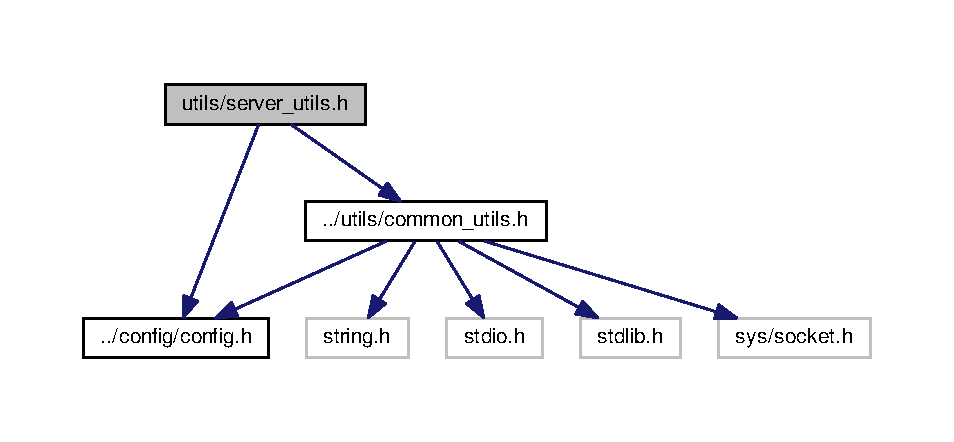
\includegraphics[width=350pt]{server__utils_8h__incl}
\end{center}
\end{figure}
This graph shows which files directly or indirectly include this file\+:
\nopagebreak
\begin{figure}[H]
\begin{center}
\leavevmode
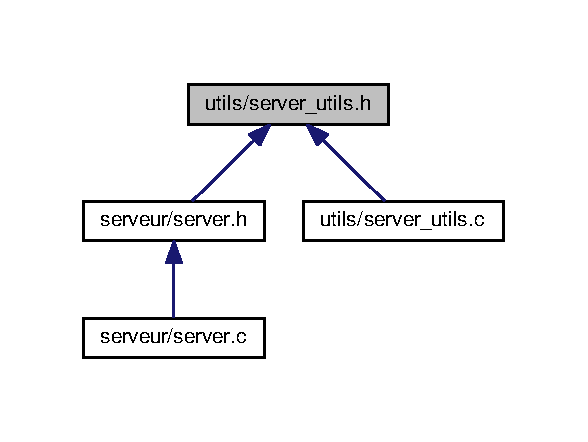
\includegraphics[width=282pt]{server__utils_8h__dep__incl}
\end{center}
\end{figure}
\subsection*{Data Structures}
\begin{DoxyCompactItemize}
\item 
struct \hyperlink{structplayer}{player}
\begin{DoxyCompactList}\small\item\em Objet chaîne de caractères. \end{DoxyCompactList}\end{DoxyCompactItemize}
\subsection*{Typedefs}
\begin{DoxyCompactItemize}
\item 
typedef struct \hyperlink{structplayer}{player} \hyperlink{server__utils_8h_a0bc8a5f0a35a8d17192faca0fcf70422}{player}
\end{DoxyCompactItemize}
\subsection*{Functions}
\begin{DoxyCompactItemize}
\item 
void \hyperlink{server__utils_8h_a529115954aec3d5719dad00b8269e4c3}{broadcast} (int msg\+\_\+code, char $\ast$payload, \hyperlink{structplayer}{player} $\ast$recipients, int rcp\+\_\+count)
\begin{DoxyCompactList}\small\item\em Diffusion du message envoyé au serveur. \end{DoxyCompactList}\item 
void \hyperlink{server__utils_8h_ab74249eacaeafc99ac0f9abc469690b6}{broadcast\+\_\+light} (int msg\+\_\+code, \hyperlink{structplayer}{player} $\ast$recipients, int rcp\+\_\+count)
\begin{DoxyCompactList}\small\item\em Diffusion du message envoyé au serveur sans le corps du message. \end{DoxyCompactList}\item 
void \hyperlink{server__utils_8h_aaece625fb465cccd16f2dc9d565742d3}{extract\+\_\+player\+\_\+nickname} (char $\ast$$\ast$msg, char $\ast$nickname)
\begin{DoxyCompactList}\small\item\em Fonction qui extrait le nom du joueur envoyé au serveur. \end{DoxyCompactList}\item 
int \hyperlink{server__utils_8h_ab7cc3806641017bc96af6fd10cabba98}{rand\+\_\+range} (int upper\+\_\+limit)
\begin{DoxyCompactList}\small\item\em Fonction qui génère un nombre aléatoire dans le max de upperlimite. \end{DoxyCompactList}\item 
\hyperlink{config_8h_a1062901a7428fdd9c7f180f5e01ea056}{bool} \hyperlink{server__utils_8h_a5dc1c39eb1f151b25bd0a5067aa8b594}{array\+\_\+contains} (int $\ast$haystack, int needle, int length)
\end{DoxyCompactItemize}


\subsection{Detailed Description}
Projet de M\+C\+S3 2016 2017. 

\begin{DoxyAuthor}{Author}
B\+E\+N\+C\+H\+I\+HA -\/ S\+A\+L\+E\+N\+G\+RO -\/ L\+E\+F\+O\+RT 
\end{DoxyAuthor}
\begin{DoxyVersion}{Version}
1 
\end{DoxyVersion}
\begin{DoxyDate}{Date}
D\+E\+C\+E\+M\+B\+RE -\/ J\+A\+N\+V\+I\+ER
\end{DoxyDate}
Fichier gérant les fonctions utilisées par le serveur 

\subsection{Typedef Documentation}
\index{server\+\_\+utils.\+h@{server\+\_\+utils.\+h}!player@{player}}
\index{player@{player}!server\+\_\+utils.\+h@{server\+\_\+utils.\+h}}
\subsubsection[{\texorpdfstring{player}{player}}]{\setlength{\rightskip}{0pt plus 5cm}typedef struct {\bf player}  {\bf player}}\hypertarget{server__utils_8h_a0bc8a5f0a35a8d17192faca0fcf70422}{}\label{server__utils_8h_a0bc8a5f0a35a8d17192faca0fcf70422}


\subsection{Function Documentation}
\index{server\+\_\+utils.\+h@{server\+\_\+utils.\+h}!array\+\_\+contains@{array\+\_\+contains}}
\index{array\+\_\+contains@{array\+\_\+contains}!server\+\_\+utils.\+h@{server\+\_\+utils.\+h}}
\subsubsection[{\texorpdfstring{array\+\_\+contains(int $\ast$haystack, int needle, int length)}{array_contains(int *haystack, int needle, int length)}}]{\setlength{\rightskip}{0pt plus 5cm}{\bf bool} array\+\_\+contains (
\begin{DoxyParamCaption}
\item[{int $\ast$}]{haystack, }
\item[{int}]{needle, }
\item[{int}]{length}
\end{DoxyParamCaption}
)}\hypertarget{server__utils_8h_a5dc1c39eb1f151b25bd0a5067aa8b594}{}\label{server__utils_8h_a5dc1c39eb1f151b25bd0a5067aa8b594}
\index{server\+\_\+utils.\+h@{server\+\_\+utils.\+h}!broadcast@{broadcast}}
\index{broadcast@{broadcast}!server\+\_\+utils.\+h@{server\+\_\+utils.\+h}}
\subsubsection[{\texorpdfstring{broadcast(int msg\+\_\+code, char $\ast$payload, player $\ast$recipients, int rcp\+\_\+count)}{broadcast(int msg_code, char *payload, player *recipients, int rcp_count)}}]{\setlength{\rightskip}{0pt plus 5cm}void broadcast (
\begin{DoxyParamCaption}
\item[{int}]{msg\+\_\+code, }
\item[{char $\ast$}]{payload, }
\item[{{\bf player} $\ast$}]{recipients, }
\item[{int}]{rcp\+\_\+count}
\end{DoxyParamCaption}
)}\hypertarget{server__utils_8h_a529115954aec3d5719dad00b8269e4c3}{}\label{server__utils_8h_a529115954aec3d5719dad00b8269e4c3}


Diffusion du message envoyé au serveur. 


\begin{DoxyParams}{Parameters}
{\em msg\+\_\+code} & \\
\hline
{\em $\ast$payload} & \\
\hline
{\em $\ast$recipients} & \\
\hline
{\em rcp\+\_\+count} & \\
\hline
\end{DoxyParams}
\begin{DoxyReturn}{Returns}
V\+O\+ID 
\end{DoxyReturn}
\index{server\+\_\+utils.\+h@{server\+\_\+utils.\+h}!broadcast\+\_\+light@{broadcast\+\_\+light}}
\index{broadcast\+\_\+light@{broadcast\+\_\+light}!server\+\_\+utils.\+h@{server\+\_\+utils.\+h}}
\subsubsection[{\texorpdfstring{broadcast\+\_\+light(int msg\+\_\+code, player $\ast$recipients, int rcp\+\_\+count)}{broadcast_light(int msg_code, player *recipients, int rcp_count)}}]{\setlength{\rightskip}{0pt plus 5cm}void broadcast\+\_\+light (
\begin{DoxyParamCaption}
\item[{int}]{msg\+\_\+code, }
\item[{{\bf player} $\ast$}]{recipients, }
\item[{int}]{rcp\+\_\+count}
\end{DoxyParamCaption}
)}\hypertarget{server__utils_8h_ab74249eacaeafc99ac0f9abc469690b6}{}\label{server__utils_8h_ab74249eacaeafc99ac0f9abc469690b6}


Diffusion du message envoyé au serveur sans le corps du message. 


\begin{DoxyParams}{Parameters}
{\em msg\+\_\+code} & \\
\hline
{\em $\ast$payload} & \\
\hline
{\em $\ast$recipients} & \\
\hline
{\em rcp\+\_\+count} & \\
\hline
\end{DoxyParams}
\begin{DoxyReturn}{Returns}
V\+O\+ID 
\end{DoxyReturn}
\index{server\+\_\+utils.\+h@{server\+\_\+utils.\+h}!extract\+\_\+player\+\_\+nickname@{extract\+\_\+player\+\_\+nickname}}
\index{extract\+\_\+player\+\_\+nickname@{extract\+\_\+player\+\_\+nickname}!server\+\_\+utils.\+h@{server\+\_\+utils.\+h}}
\subsubsection[{\texorpdfstring{extract\+\_\+player\+\_\+nickname(char $\ast$$\ast$msg, char $\ast$nickname)}{extract_player_nickname(char **msg, char *nickname)}}]{\setlength{\rightskip}{0pt plus 5cm}void extract\+\_\+player\+\_\+nickname (
\begin{DoxyParamCaption}
\item[{char $\ast$$\ast$}]{msg, }
\item[{char $\ast$}]{nickname}
\end{DoxyParamCaption}
)}\hypertarget{server__utils_8h_aaece625fb465cccd16f2dc9d565742d3}{}\label{server__utils_8h_aaece625fb465cccd16f2dc9d565742d3}


Fonction qui extrait le nom du joueur envoyé au serveur. 


\begin{DoxyParams}{Parameters}
{\em signum} & numéro du signal \\
\hline
\end{DoxyParams}
\begin{DoxyReturn}{Returns}
V\+O\+ID 
\end{DoxyReturn}
\index{server\+\_\+utils.\+h@{server\+\_\+utils.\+h}!rand\+\_\+range@{rand\+\_\+range}}
\index{rand\+\_\+range@{rand\+\_\+range}!server\+\_\+utils.\+h@{server\+\_\+utils.\+h}}
\subsubsection[{\texorpdfstring{rand\+\_\+range(int upper\+\_\+limit)}{rand_range(int upper_limit)}}]{\setlength{\rightskip}{0pt plus 5cm}int rand\+\_\+range (
\begin{DoxyParamCaption}
\item[{int}]{upper\+\_\+limit}
\end{DoxyParamCaption}
)}\hypertarget{server__utils_8h_ab7cc3806641017bc96af6fd10cabba98}{}\label{server__utils_8h_ab7cc3806641017bc96af6fd10cabba98}


Fonction qui génère un nombre aléatoire dans le max de upperlimite. 

Fonction qui vérifie si une carte est présente dans le tableau.


\begin{DoxyParams}{Parameters}
{\em upper\+\_\+limit} & \\
\hline
\end{DoxyParams}
\begin{DoxyReturn}{Returns}
int
\end{DoxyReturn}

\begin{DoxyParams}{Parameters}
{\em $\ast$haystack} & \\
\hline
{\em needle} & \\
\hline
{\em length} & \\
\hline
\end{DoxyParams}
\begin{DoxyReturn}{Returns}
bool 
\end{DoxyReturn}

%--- End generated contents ---

% Index
\backmatter
\newpage
\phantomsection
\clearemptydoublepage
\addcontentsline{toc}{chapter}{Index}
\printindex

\end{document}
